\documentclass[12pt,a4paper]{report}

\usepackage[utf8]{inputenc}
\usepackage[french]{babel}
\usepackage[autolanguage]{numprint}
\usepackage[T1]{fontenc}
\usepackage{amsfonts,amsmath,amssymb}
\usepackage{bigints}

\DeclareMathOperator{\arcsinh}{arcsinh}
\DeclareMathOperator{\arccosh}{arccosh}
\DeclareMathOperator{\arctanh}{arctanh}

\usepackage[pdftex]{pict2e}
\usepackage[dvipsnames]{xcolor}
\usepackage{graphicx}

\graphicspath{
    {chapters/graphics/}
	{chapters/exercices/graphics/}
}

\setcounter{tocdepth}{3}

\setlength{\paperwidth}{21cm}
\setlength{\paperheight}{29.7cm}
\setlength{\evensidemargin}{0cm}
\setlength{\oddsidemargin}{-0.5cm}
\setlength{\topmargin}{-2cm}
\setlength{\headsep}{0.15cm}
\setlength{\headheight}{0.7cm}
\setlength{\textheight}{25cm}
\setlength{\textwidth}{18cm}

\newcommand{\be}{\begin{equation}}
\newcommand{\ee}{\end{equation}}
\newcommand{\bea}{\begin{eqnarray}}
\newcommand{\eea}{\end{eqnarray}} 
\newcommand{\bc}{\begin{center}}
\newcommand{\ec}{\end{center}}
\newcommand{\bed}{\begin{description}}
\newcommand{\eed}{\end{description}}

\newcommand{\trint}{\mathop{\int\!\!\!\int\!\!\!\int}\limits}
\newcommand{\dint}{\mathop{\int\!\!\!\int}\limits}

\title{\'Etapes de calcul et d\'emonstrations du tome 1 <<~M\'ecanique~>>  de Physique Th\'eorique de L. Landau \&  E. Lifchitz}
\author{S\'ebastien Majerowicz}
\date{2023 -- 2024}

\begin{document}

\maketitle

\begin{abstract}
Ce document est une aide pour la compr\'ehension du premier livre des c\'el\`ebres cours de Landau \& Lifschitz au travers de la d\'emonstration des formules et de la r\'esolution des exercices propos\'es.
\end{abstract}

\tableofcontents
\listoffigures

\clearpage
\pagenumbering{arabic}
\setcounter{page}{1}

\chapter{\'Equations du mouvement}
\section{Coordonn\'ees g\'en\'eralis\'ees}

Pour un point mat\'eriel, nous avons en coordonn\'ees cart\'esiennes :
\begin{itemize}
\item le rayon vecteur tel que :
	\be
		\vec{r} = \begin{pmatrix} x \\ y \\ z \end{pmatrix}
	\ee
\item la vitesse telle que :
	\be
		\vec{v} = \dfrac{{\rm d}\vec{r}}{{\rm dt}}
	\ee
\item l'acc\'el\'eration telle que :
	\be
		\vec{a} = \dfrac{{\rm d}\vec{v}}{{\rm d}t} = \frac{{\rm d}^{2}\vec{r}}{{\rm dt^{2}}}
	\ee
\end{itemize}

Les coordonn\'ees cart\'esiennes ne sont pas toujours les plus adapt\'ees. Un autre syt\`eme de coordonn\'ees peut \^etre plus commode \`a utiliser. Il convient de choisir alors $s$ grandeurs quelconques $\begin{Bmatrix}q_{i}\end{Bmatrix}^{s}_{1}$ pour d\'efinir la position d'un syst\`eme ($s$ degr\'es de libert\'es), ce sont ses \emph{coordonn\'ees g\'en\'eralis\'ees} et les d\'riv\'ees $\begin{Bmatrix}\dot{q}_{i}\end{Bmatrix}^{s}_{1}$, ses \emph{vitesses g\'en\'eralis\'ees}.

Les relations qui lient les acc\'el\'erations aux coordonn\'ees et aux vitesses sont appel\'ees les \emph{\'equations du mouvement}.

\section{Le principe de moindre action}

La formule la plus g\'en\'erale de la loi du mouvement des syst\`emes mécaniques est celle du \emph{principe de moindre action} (ou principe de Hamilton). Il introduit la \emph{fonction de Lagrange} d\'efinie telle que :
\be
	L(\begin{Bmatrix}q_{i}\end{Bmatrix}^{s}_{1},\begin{Bmatrix}\dot{q}_{i}\end{Bmatrix}^{s}_{1}, {\rm t}) = L(q,\dot{q},{\rm t})
\ee
Entre les instants ${\rm t}_{1}$ et ${\rm t}_{2}$, le système se meut de telle mani\`ere que l'\emph{action} :
\be
	S = \int_{{\rm t}_{1}}^{{\rm t}_{2}} L(q,\dot{q},{\rm t}) d{\rm t} \label{EQ:2_1}
\ee
ait la plus petite valeur possible.

Partons d'un seul degr\'e de libert\'e et d\'efinissons $q=q({\rm t})$ telle que $S$ soit minimale. Cela signifie que $S$ a une valeur plus grande si :
\be
	q({\rm t}) \rightarrow q({\rm t})+\delta q({\rm t}) \label{EQ:2_2}
\ee
avec $\delta q({\rm t})$ est la variation de $q({\rm t})$. Or en ${\rm t}_{1}$ et ${\rm t}_{2}$, toutes les fonctions $q({\rm t})$ doivent avoir des valeurs identiques (les trajectoires diff\`erent mais pas les conditions initiales, ni finales). Donc $\forall q({\rm t})$, nous avons :
\be
	\delta q({\rm t}_{1})=\delta q({\rm t}_{2})=0 \label{EQ:2_3}
\ee
De plus $\dot{q}=\dfrac{{\rm d}q}{\rm dt}$ dont $\dfrac{{\rm d}(q+\delta q)}{\rm dt}=\dot{q}+\delta\dot{q}$.
\be
	S(q+\delta q, \dot{q}+\delta \dot{q}, {\rm t}) - S(q,\dot{q},{\rm t}) = \delta S = \int_{{\rm t}_{1}}^{{\rm t}_{2}} L(q+\delta q, \dot{q}+\delta \dot{q}, {\rm t}) d{\rm t} - \int_{{\rm t}_{1}}^{{\rm t}_{2}} L(q,\dot{q},{\rm t}) d{\rm t}
\ee
Or par d\'efinition, nous avons :
\be
	\delta L(q,\dot{q},{\rm t}) = \dfrac{\partial L}{\partial q}\delta q + \dfrac{\partial L}{\partial \dot{q}}\delta \dot{q} + \dfrac{\partial L}{\partial {\rm t}}\delta {\rm t}
\ee
Mais puisque $\delta {\rm t}=0$, cela donne, au premier ordre (développement en s\'erie de Taylor) :
\be
	L(q+\delta q, \dot{q}+\delta \dot{q}, {\rm t}) \approx L(q,\dot{q},{\rm t}) + \dfrac{\partial L}{\partial q}\delta q + \dfrac{\partial L}{\partial \dot{q}}\delta \dot{q}
\ee
ou encore, le principe de moindre action peut s'\'ecrire :
\be
	\delta S = \delta \int_{{\rm t}_{1}}^{{\rm t}_{2}} L(q,\dot{q},{\rm t}) d{\rm t} = 0 \label{EQ:2_4}
\ee
et, de facto :
\be
	\int_{{\rm t}_{1}}^{{\rm t}_{2}} \left(\dfrac{\partial L}{\partial q}\delta q + \dfrac{\partial L}{\partial \dot{q}}\delta \dot{q}\right) {\rm dt} = 0
\ee
Ensuite, remarquons que :
\be
	\delta \dot{q} = \delta\left(\dfrac{{\rm d}q}{{\rm dt}}\right) = \dfrac{{\rm d}\delta q}{{\rm dt}}
\ee
L'\'equation \ref{EQ:2_4} devient alors :
\be
	\int_{{\rm t}_{1}}^{{\rm t}_{2}} \dfrac{\partial L}{\partial q}\delta q + \dfrac{\partial L}{\partial \dot{q}}\dfrac{{\rm d}\delta q}{{\rm dt}} \delta {\rm t} = 0
\ee
En se rappelant l'intégration par parties de Brook Taylor qui dit que :
\be
	\int_{a}^{b} u(x)v'(x){\rm dx} = \left[u(x)v(x)\right]_{a}^{b} - \int_{a}^{b} u'(x)v(x){\rm dx}
\ee
alors :
\be
	\int_{{\rm t}_{1}}^{{\rm t}_{2}} \dfrac{\partial L}{\partial \dot{q}}\dfrac{{\rm d}\delta q}{{\rm dt}} \delta {\rm t} = \left[\dfrac{\partial L}{\partial \dot{q}}\delta q\right]_{{\rm t}_{1}}^{{\rm t}_{2}} - \int_{{\rm t}_{1}}^{{\rm t}_{2}} \dfrac{{\rm d}}{{\rm dt}}\left(\dfrac{\partial L}{\partial \dot{q}}\right) \delta q{\rm dt}
\ee
L'\'equation \ref{EQ:2_4} s'\'ecrit donc :
\bea
	\delta S & = & \int_{{\rm t}_{1}}^{{\rm t}_{2}} \dfrac{\partial L}{\partial q}\delta q {\rm dt} + \left[\dfrac{\partial L}{\partial \dot{q}}\delta q\right]_{{\rm t}_{1}}^{{\rm t}_{2}} - \int_{{\rm t}_{1}}^{{\rm t}_{2}} \dfrac{{\rm d}}{{\rm dt}}\left(\dfrac{\partial L}{\partial \dot{q}}\right) \delta q{\rm dt} \nonumber \\
	& = & \left[\dfrac{\partial L}{\partial \dot{q}}\delta q\right]_{{\rm t}_{1}}^{{\rm t}_{2}} - \int_{{\rm t}_{1}}^{{\rm t}_{2}} \left(\dfrac{\partial L}{\partial q}-\dfrac{{\rm d}}{{\rm dt}}\left(\dfrac{\partial L}{\partial \dot{q}}\right)\right) \delta q{\rm dt} \label{EQ:2_5}
\eea
or l'application de \ref{EQ:2_3} dans \ref{EQ:2_5} implique directement :
\be
	\delta S = \int_{{\rm t}_{1}}^{{\rm t}_{2}} \left(\dfrac{\partial L}{\partial q}-\dfrac{{\rm d}}{{\rm dt}}\left(\dfrac{\partial L}{\partial \dot{q}}\right)\right) \delta q{\rm dt}
\ee
Le principe de moindre action donne $\forall q$, $\delta S = 0$ et l'expression ci-dessus doit \^etre valide quelque soit la valeur de $\delta q$. Cela a pour cons\'equence :
\be
	\dfrac{\partial L}{\partial q}-\dfrac{{\rm d}}{{\rm dt}}\left(\dfrac{\partial L}{\partial \dot{q}}\right) = 0
\ee
ce qui donne les \emph{\'equations de Lagrange} lorsqu'il y a $s$ degr\'es de libert\'e :
\be
	\forall i \in \left(1, 2, \ldots, s\right), \dfrac{\partial L}{\partial q_{i}}-\dfrac{{\rm d}}{{\rm dt}}\left(\dfrac{\partial L}{\partial \dot{q_{i}}}\right) = 0\label{EQ:2_6}
\ee
c'est-\`a-dire $s$ \'equations diff\'erentielles du second ordre à $s$ inconnues, $q_{i}({\rm t})$.

Si (A) et (B) sont deux syst\`emes ferm\'es suffisamment \'eloign\'es pour n\'egliger leur interaction mutuelle alors :
\be
	\lim L = L_{A} + L_{B} \label{EQ:2_7}
\ee
Il s'agit de l'additivit\'e de la fonction de Lagrange. De la m\^eme mani\`ere, la multiplication par une constante de la fonction de Lagrange d'un syst\`eme ferm\'e n'influe pas les \'equations du mouvement.

Une derni\`ere remarque en consid\'erant la fonction de Lagrange $L'$ telle que :
\be
	L'(q,\dot{q},t)=L(q,\dot{q},t) + \frac{{\rm d}f(q,{\rm t})}{{\rm dt}} \label{EQ:2_8}
\ee
alors les int\'egrales \ref{EQ:2_1} donnent :
\bea
	S' & = & \int_{{\rm t}_{1}}^{{\rm t}_{2}} L'(q,\dot{q},{\rm t}) d{\rm t} = \int_{{\rm t}_{1}}^{{\rm t}_{2}} L(q,\dot{q},{\rm t}) d{\rm t} + \int_{{\rm t}_{1}}^{{\rm t}_{2}} \dfrac{{\rm d}f(q,{\rm t})}{{\rm dt}} d{\rm t} \nonumber \\
	& = & S + \int_{{\rm t}_{1}}^{{\rm t}_{2}} {\rm d}f(q,{\rm t}) = S + f(q({\rm t}_{2})) - f(q({\rm t}_{1}))
\eea
et impliquent que le principe de moindre action $\delta S = 0$ co\"incide avec $\delta S' = 0$. Ainsi, la fonction de Lagrange n'est d\'etermin\'ee qu'\`a la d\'eriv\'ee totale d'une fonction quelconque des coordonn\'ees et du temps.

\section{Le principe de relativit\'e de Galil\'ee}

Il est n\'ecessaire de choisir un syst\`eme de r\'ef\'erence pour \'etudier les ph\'enom\`enes m\'ecaniques et il est pr\'ef\'erable de le choisir afin que les lois de la m\'ecanique y soit les plus simples possibles. Et il est toujours possible de trouver un r\'ef\'erentiel tel que l'espace est homog\`ene et isotrope et le temps uniforme. En d'autres termes, la fonction de Lagrange d'un point mat\'eriel se mouvant librement dans un syst\`eme galil\'een en coordonn\'ees cart\'esiennes :
\begin{itemize}
	\item homog\'en\'it\'e de l'espace : $L(\vec{r},\vec{v},{\rm t}) \Rightarrow L(\vec{v},{\rm t})$
	\item uniformit\'e du temps : $L(\vec{v},{\rm t}) \Rightarrow L(\vec{v})$
	\item isotropie de l'espace : $L(\vec{v}) \Rightarrow L(\lVert\vec{v}\rVert)$
\end{itemize}
En r\'esum\'e, nous avons :
\be
	L = L(\vec{v}^{\,2}) \label{EQ:3_1}
\ee
ce qui implique que $\dfrac{\partial L}{\partial \vec{r}} = 0$. Et par application des \'equations de Lagrange (\ref{EQ:2_6}), nous avons :
\be
	\dfrac{{\rm d}}{{\rm dt}}\left(\dfrac{\partial L}{\partial \vec{v}}\right) = 0
\ee
et comme la fonction de Lagrange n'est fonction que de la vitesse, ou encore $\dfrac{\partial L({\vec{v}}^{\,2})}{\partial \vec{v}} \propto \vec{v}$ (voir \ref{EQ:3_1}), dans ce cas alors :
\be
	\vec{v} = \vec{Cte} \label{EQ:3_2}
\ee
Dans un r\'ef\'erentiel galil\'een, tout mouvement libre s'effectue donc \`a une vitesse constante en grandeur et en direction. C'est la \emph{loi de l'inertie}. Supposons deux r\'ef\'erentiels galil\'eens ($K$) et ($K'$) tels que $\vec{KK'}=\vec{V}{\rm t}$. Alors $\vec{r}=\vec{KK'}+\vec{r'}$, soit :
\be
	\vec{r} = \vec{r'} + \vec{V}{\rm t} \label{EQ:3_3}
\ee
En M\'ecanique classique, le temps est absolu, aussi :
\be
	{\rm t} = {\rm t'} \label{EQ:3_4}
\ee
Les formules (\ref{EQ:3_3}) et (\ref{EQ:3_4}) sont les \emph{transformations de Galil\'ee}.

\section{Fonction de Lagrange d'un point mat\'eriel libre}

Consid\'erons le mouvement libre d'un point mat\'eriel dans un syst\`eme gali\'een. Cela implique \ref{EQ:3_1}, soit $L = L(v^{2})$. Avec un r\'ef\'erentiel $(K)$ qui se d\'eplace par rapport \`a un autre r\'ef\'erentiel (K') telle que $\vec{v'}=\vec{v} + \vec{\epsilon}$, nous avons :
\bea
L' = L(\vec{v'}^{\,2}) & = & L(\vec{v}^{\,2} + 2\vec{v}.\vec{\epsilon} + \vec{\epsilon}^{\,2}) \nonumber \\
 & = & L(\vec{v}^{\,2}) + \dfrac{\partial L}{\partial \vec{v}^{\,2}}2\vec{v}.\vec{\epsilon}
\eea
en supprimant les ordres sup\'erieurs à 2 en $\vec{\epsilon}$ dans le d\'eveloppement en s\'erie de Taylor de :
\be
	L(\vec{v}^{\,2} + 2\vec{v}.\vec{\epsilon} + \vec{\epsilon}^{\,2}) \approx L(\vec{v}^{\,2} + \dfrac{\partial L}{\partial \vec{v}^{\,2}}.(2\vec{v}.\vec{\epsilon}+\vec{\epsilon}^{\,2}) + \dfrac{\partial L}{2\partial \vec{v}^{\,4}}.(2\vec{v}.\vec{\epsilon}+\vec{\epsilon}^{\,2})^{2} + \ldots
\ee
En reprenant la fonction de Lagrange qui peut se d\'efinir comme (\ref{EQ:2_8}), nous pouvons pos\'e :
\bea
	\dfrac{\partial L}{\partial \vec{v}^{\,2}}2\vec{v}.\vec{\epsilon} & = & \dfrac{{\rm d}f(\vec{r},t)}{{\rm dt}} \nonumber \\
	\Leftrightarrow 2\dfrac{\partial L}{\partial \vec{v}^{\,2}}\dfrac{{\rm d}\vec{r}}{{\rm dt}}.\vec{\epsilon} & = & \dfrac{{\rm d}f(\vec{r},t)}{{\rm dt}} \nonumber \\
	\Leftrightarrow 2\dfrac{\partial L}{\partial \vec{v}^{\,2}}\dfrac{{\rm d}(\vec{r}.\vec{\epsilon})}{{\rm dt}} & = & \dfrac{{\rm d}f(\vec{r},t)}{{\rm dt}}
\eea
n'est vraie que si et seulement si $\dfrac{\partial L}{\partial \vec{v}^{\,2}} = \alpha$, avec $\alpha$ une constante. Or nous avons \ref{EQ:3_1}, qui implique :
\be
	L = L(\vec{v}^{\,2}) = \alpha\vec{v}^{\,2}
\ee
\chapter{Lois de conservation}

\section{\'Energie}\label{PAR:6}

Les \emph{int\'egrales premi\`eres} ou \emph{int\'egrales du mouvement}, sont les fonctions de $q_{i}$ et $\dot{q}_{i}$ qui conservent une valeur constante au cours du mouvement. Elles sont additives, c'est-\`a-dire qu'avant et après une int\'eraction, leur somme garde une valeur identique.

Commen\c{c}ons par l'int\'egrale premi\`ere qui d\'ecoule de l'\emph{uniformi\'e du temps}.

Pour un syst\`eme ferm\'e \`a $s$ degr\'es de libert\'e, nous avons :
\be
	\dfrac{\mathrm{d}L}{\mathrm{dt}} = \sum_{i=1}^{s}\dfrac{\partial L}{\partial q_{i}}\dfrac{\mathrm{d} q_{i}}{\mathrm{dt}} + \sum_{i=1}^{s}\dfrac{\partial L}{\partial \dot{q}_{i}}\dfrac{\mathrm{d}\dot{q}_{i}}{\mathrm{dt}} + \dfrac{\partial L}{\partial \mathrm{t}}
\ee
L'uniformit\'e du temps donne $\dfrac{\partial L}{\partial \mathrm{t}} = 0$ et en utilisant l'\'equation (\ref{EQ:2_6}), nous avons :
\bea
	\dfrac{\mathrm{d}L}{\mathrm{dt}} & = & \sum_{i=1}^{s}\dfrac{\mathrm{d}}{\mathrm{dt}}\left(\dfrac{\partial L}{\partial \dot{q}_{i}}\dot{q}_{i}\right) + \sum_{i=1}^{s}\dfrac{\partial L}{\partial \dot{q}_{i}}\ddot{q}_{i} \nonumber \\
	& = & \sum_{i=1}^{s}\dfrac{\mathrm{d}}{\mathrm{dt}}\left(\dfrac{\partial L}{\partial \dot{q}_{i}}\dot{q}_{i}\right) \nonumber \\
	0 & = & \dfrac{\mathrm{d}}{\mathrm{dt}}\left(\sum_{i=1}^{s}\dfrac{\partial L}{\partial \dot{q}_{i}}\dot{q}_{i} - L\right)
\eea
Par cons\'equent, la quantit\'e :
\be
	E = \sum_{i=1}^{s}\dfrac{\partial L}{\partial \dot{q}_{i}}\dot{q}_{i} - L \label{EQ:6_1}
\ee
est constante dans le temps pour un syst\`eme ferm\'e. $E$ est l'\emph{\'energie} du syst\`eme. Et puisque la fonction de Lagrange est additive, l'\'energie l'est aussi. Les syst\`emes m\'ecaniques dont l'\'energie se conserve sont appel\'es \emph{syst\`emes conservatifs}. Enfin, si le syst\`eme est plac\'e dans un champ ext\'erieur constant par rapport au temps alors la loi de conservation de l'\'energie reste valable car la fonction de Lagrange est implicitement ind\'ependant du temps.

\`A partir de l'\'equation (\ref{EQ:5_1}, nous pouvons \'ecrire :
\be
	\sum_{i=1}^{s}\dfrac{\partial L}{\partial\dot{q}_{i}}\dot{q}_{i} = \sum_{i=1}^{s}\dfrac{\partial (T-U)}{\partial\dot{q}_{i}}\dot{q}_{i} = \sum_{i=1}^{s}\dfrac{\partial T}{\partial\dot{q}_{i}}\dot{q}_{i}
\ee
car l'\'energie potentielle $U$ ne d\'epend que des coordonn\'ees (voire du temps).
Nous savons que l'\'energie cin\'etique $T = f(\dot{q}^{2})$. Or pour une fonction homog\`ene de degr\'e $\alpha$, telle $f(t.x) = t^{\alpha}f(x)$, alors le th\'eor\`eme d'Euler donne pour cette fonction :
\be
	\sum_{i} x_{i}\dfrac{\partial f(x)}{\partial x_{i}} = \alpha f(x)
\ee
Appliqu\'ee \`a l'\'energie cin\'etique, cela donne :
\be
	\sum_{i=1}^{s}\dfrac{\partial T}{\partial\dot{q}_{i}}\dot{q}_{i} = 2T = \sum_{i=1}^{s}\dfrac{\partial L}{\partial\dot{q}_{i}}\dot{q}_{i} \label{EQ:6_1_1}
\ee
ce qui permet de conclure \`a, en compl\'etant l'\'equation (\ref{EQ:6_1}) :
\be
	E = T(q,\dot{q}) + U(q) \label{EQ:6_2}
\ee
soit en coordonn\'ees cart\'esiennes :
\be
	E = \sum_{a}\dfrac{m_{a}\vec{v}_{a}^{\,2}}{2} + U(\begin{Bmatrix}\vec{r}_{i}\end{Bmatrix}_{1}^{s}) \label{EQ:6_3}
\ee

\section{Impulsion}

Apr\`es l'unformit\'e du temps, nous allons \'etudier les cons\'equences de l'homog\'en\'eit\'e de l'espace. Dans ce cadre, les propri\'et\'es m\'ecaniques d'un syst\`eme ferm\'e ne changent pas lors d'un d\'eplacement parall\`ele du syst\`eme dans son entier. Supposons ainsi que la fonction de Lagrange reste inchang\'ee pour un d\'eplacement infinit\'esimal tel que : $\vec{r}_{a} \rightarrow \vec{r}_{a} + \vec{\epsilon}$, i.e. $\delta L = 0$ :
\bea
	\delta L(\vec{r}_{a},\vec{v}_{a}) & = & \sum_{a}\dfrac{\partial L}{\partial\vec{r}_{a}}\delta\vec{r}_{a} + \sum_{a}\dfrac{\partial L}{\partial\vec{v}_{a}}\delta\vec{v}_{a} \nonumber \\
	& = & \sum_{a}\dfrac{\partial L}{\partial\vec{r}_{a}}\vec{\epsilon} \text{ puisque }\delta\vec{v}_{a} = \vec{0} \nonumber \\
\eea
donc $\delta L = 0$ est \'equivalent \`a :
\bea
	\forall \vec{\epsilon}\text{, }\sum_{a}\dfrac{\partial L}{\partial\vec{r}_{a}}\vec{\epsilon} & = & 0 \nonumber \\
	\forall \vec{\epsilon}\text{, }\vec{\epsilon}\cdot\sum_{a}\dfrac{\partial L}{\partial\vec{r}_{a}} & = & 0 \nonumber \\
	\Leftrightarrow \sum_{a}\dfrac{\partial L}{\partial\vec{r}_{a}} & = & 0 \label{EQ:7_1}
\eea
Or les \'equations de Lagrange (\ref{EQ:5_2}) donnent :
\bea
	\dfrac{\mathrm{d}}{\mathrm{dt}}\left(\dfrac{\partial L}{\partial \vec{v}_{a}}\right) & = & \dfrac{\partial L}{\partial \vec{r}_{a}} \nonumber \\
	\Leftrightarrow \sum_{a}\left(\dfrac{\mathrm{d}}{\mathrm{dt}}\left(\dfrac{\partial L}{\partial \vec{v}_{a}}\right)\right) & = & \sum_{a}\left(\dfrac{\partial L}{\partial \vec{r}_{a}}\right) \nonumber
\eea
En appliquant l'\'equation (\ref{EQ:7_1}), nous avons :
\be
	\sum_{a}\left(\dfrac{\mathrm{d}}{\mathrm{dt}}\left(\dfrac{\partial L}{\partial \vec{v}_{a}}\right)\right) = \dfrac{\mathrm{d}}{\mathrm{dt}}\sum_{a}\left(\dfrac{\partial L}{\partial \vec{v}_{a}}\right) = \vec{0}
\ee
Ainsi, dans un syst\`eme ferm\'e, la quantit\'e vectorielle :
\be
	\vec{P} = \sum_{a}\dfrac{\partial L}{\partial \vec{v}_{a}} \label{EQ:7_2}
\ee
est inchang\'ee pendant le mouvement. Le vecteur $\vec{P}$ est l'\emph{impulsion}\footnote{Anciennement appel\'ee \emph{quantit\'e de mouvement}} du syt\`eme. En utilisant l'\'equation (\ref{EQ:5_1}), nous obtenons :
\bea
	L & = & \sum_{a}\dfrac{m_{a}\vec{v}_{a}^{\,2}}{2} - U(\begin{Bmatrix}\vec{r}_{a}\end{Bmatrix}_{1}^{s}) \nonumber \\
	\Rightarrow \dfrac{\partial L}{\partial \vec{v}_{a}} & = & \dfrac{m_{a}}{2}\dfrac{2\partial\vec{v}_{a}}{\partial\vec{v}_{a}} - \dfrac{\partial U}{\partial\vec{v}_{a}} \nonumber \\
	& = & m_{a}\vec{v}_{a}
\eea
Ainsi :
\be
	\vec{P} = \sum_{a}m_{a}\vec{v}_{a} \label{EQ:7_3}
\ee
avec $\vec{P} = \sum_{a}\vec{p}_{a}$ pour un syst\`eme ferm\'e en l'absence de champ ext\'erieur.

Supposons l'existence d'un champ ext\'erieur telle que $U\rightarrow U(z)$ en coordonn\'ees cart\'esiennes, les \'equations de Newton (\ref{EQ:5_3}) donnent :
\bea
	m_{a}\dfrac{\mathrm{d}v_{x}}{\mathrm{d}x} & = & - \dfrac{\partial U}{\partial x} = 0 \nonumber \\
	m_{a}\dfrac{\mathrm{d}v_{y}}{\mathrm{d}y} & = & - \dfrac{\partial U}{\partial y} = 0 \nonumber \\
	m_{a}\dfrac{\mathrm{d}v_{z}}{\mathrm{d}z} & = & - \dfrac{\partial U}{\partial z} \nonumber
\eea
et donc, dans ce cas, $P_{x}$ et $P_{y}$ se conservent donc.

Une cons\'equence de l'\'equation (\ref{EQ:7_1}) en accord avec celle de (\ref{EQ:5_4}) pour la force $\vec{F}_{a}$ agissant sur le point mat\'eriel $a$ est que :
\be
	\sum_{a}\vec{F}_{a} = \vec{0} \label{EQ:7_4}
\ee
i.e. que la somme de toutes les forces s'exer\c{c}ant sur toutes les particules d'un syst\`eme ferm\'e est absolument nulle. Dans le cas particulier de deux particules, il y a $\vec{F}_{1} + \vec{F}_{2} = \vec{0}$. Les deux forces sont \'egales mais oppos\'ees, il s'agit de la loi de l'\'egalit\'e entre l'action et la r\'eaction.

Dans le cadre du mouvement d\'ecrit par les coordonn\'ees g\'en\'eralis\'ees, nous avons :
\begin{itemize}
	\item les \emph{impulsions g\'en\'eralis\'ees} :
	\be
		p_{i} = \dfrac{\partial L}{\partial\dot{q}_{i}} \label{EQ:7_5}
	\ee
	\item les \emph{forces g\'en\'eralis\'ees} :
	\be
		F_{i} = \dfrac{\partial L}{\partial q_{i}} \label{EQ:7_6}
	\ee
	\item les \'equations de Lagrange :
	\be
		\dot p_{i} = F_{i} \label{EQ:7_7}
	\ee
\end{itemize}

\section{Centre d'inertie}\label{PAR:8}

Supposons deux r\'ef\'erentiels $(K)$ et $(K')$ tels que le second se meut à la vitesse $\vec{V}$ par rapport au premier. Nous avons donc $\vec{v}_{a} = \vec{v'}_{a} + \vec{V}$, soit, pour l'impulsion :
\bea
	\vec{P} = \sum_{a}m_{a}\vec{v}_{a} & = & \sum_{a}m_{a}\vec{v'}_{a} + \sum_{a}m_{a}\vec{V} \nonumber \\
	\Leftrightarrow \vec{P} & = & \vec{P'} + \vec{V}\sum_{a}m_{a} \label{EQ:8_1}
\eea
Il existe toujours un r\'ef\'erentiel $(K')$ tel que le syst\`eme est consid\'er\'e comme au repos, soit $\vec{P'} = \vec{0}$. La vitesse de ce r\'ef\'erentiel par rapport \`a $(K)$ peut s'\'ecrire :
\be
	\vec{V} = \dfrac{\vec{P}}{\sum_{a}m_{a}} = \dfrac{\sum_{a}m_{a}\vec{v}_{a}}{\sum_{a}m_{a}} \label{EQ:8_2}
\ee
et elle d\'efinit la vitesse dans son ensemble du syst\`eme m\'ecanique ayant une impulsion $\vec{P}$ non nulle. Et une analogie avec le mouvement d'un point mat\'eriel est \'evidente en posant sa masse comme $\mu = \sum_{a}m_{a}$. La masse est donc \emph{additive}.
La relation (\ref{EQ:8_2}) peut aussi s'\'ecrire comme :
\bea
	\vec{V} = \dfrac{\vec{R}}{\mathrm{dt}} & = & \dfrac{\sum_{a}m_{a}\dfrac{\vec{r}_{a}}{\mathrm{dt}}}{\sum_{a}m_{a}} = \dfrac{\mathrm{d}}{\mathrm{dt}}\left(\dfrac{\sum_{a}m_{a}\vec{r}_{a}}{\sum_{a}m_{a}}\right) \nonumber \\
	\Leftrightarrow \vec{R} & = & \dfrac{\sum_{a}m_{a}\vec{r}_{a}}{\sum_{a}m_{a}} \label{EQ:8_3}
\eea
Ainsi la vitesse d'un syst\`eme dans son ensemble est la vitesse de d\'eplacement du point de l'espace dont le rayon vecteur est d\'efini par l'\'equation (\ref{EQ:8_3}). Ce point est appel\'e \emph{centre d'inertie} du syst\`eme m\'ecanique.

Il s'agit d'une g\'en\'eralisation de la loi d'inertie \'enonc\'ee en (\ref{EQ:3_2}) pour un syst\`eme ferm\'e dont le centre d'inertie co\"incide avec le point mat\'eriel. En conclusion, pour \'etudier les propri\'et\'es m\'ecaniques d'une syst\`eme ferm\'e, il est int\'eressant de choisir le r\'ef\'erentiel dans lequel son centre d'inertie est au repos et le mouvement rectiligne et uniforme du syst\`eme peut alors \^etre occult\'e.
Soit $E_{\mathrm{int}}$ l'\'energie interne d'un syst\`eme ferm\'e au repos, elle comprend l'\'energie cin\'etiques du mouvement relatif des particules dans le syst\`eme ainsi que l'\'energie potentielle de leur int\'eraction mutuelle. L'\'energie totale d'un syst\`eme m\^u dans son ensemble par une vitesse $\vec{V}$ peut s'\'ecrire :
\be
	E = \dfrac{\mu \vec{V}^{\,2}}{2} + E_{\mathrm{int}} \label{EQ:8_4}
\ee
En effet, dans le r\'ef\'erentiel $(K)$ :
\bea
	E & = & \dfrac{1}{2}\sum_{a}m_{a}\vec{v}_{a}^{\,2} + U = \dfrac{1}{2}\sum_{a}m_{a}(\vec{v'}_{a} + \vec{V})^{\,2} + U \nonumber \\
	& = & \dfrac{1}{2}\sum_{a}m_{a}\vec{v'}_{a}^{\,2} + \dfrac{1}{2}\sum_{a}m_{a}\vec{V}^{\,2} + \sum_{a}m_{a}\vec{v'}_{a}\vec{V} + U \nonumber \\
	& = & \dfrac{\mu}{2}\vec{V} + \vec{V}\sum_{a}m_{a}\vec{v'}_{a} + \dfrac{1}{2}\sum_{a}m_{a}\vec{v'}_{a}^{\,2} + U \\
\eea
Puisque :
\bea
	E' & = & \dfrac{1}{2}\sum_{a}m_{a}\vec{v'}_{a}^{\,2} + U \nonumber \\
	\vec{P'} & = & \sum_{a}m_{a}\vec{v'}_{a} \nonumber
\eea
alors nous arrivons \`a :
\be
	E = E' + \vec{V}\cdot\vec{P'} + \dfrac{\mu}{2}\vec{V} \label{EQ:8_5}
\ee
qui est la loi de transformation de l'\'energie lors d'un changement de r\'ef\'erentiel se mouvant l'un par rapport \`a l'autre comme d\'efini. Aussi, dans le cas d'un syst\`eme m\'ecanique au repos dans le r\'ef\'erentiel $(K')$, alors $\vec{P'} = \vec{0}$  et $E'$ est l'\'energie interne de ce syst\`eme. Nous retombons alors sur l'\'equation (\ref{EQ:8_4}).

\section{Moment cinétique}

Apr\`es l'uniformit\'e du temps, l'homog\'en\'eit\'e de l'espace, nous allons \'etudier les cons\'equences de l'isotropie de l'espace. Celle-ci implique que les propri\'et\'es m\'ecaniques d'un syst\`eme ferm\'e ne changent pas lors d'une rotation. Nous consid\'erons donc que la fonction de Lagrange reste inchang\'ee lors d'une rotation infinit\'esimale.

\begin{figure}[htb!]
	\begin{center}
		\begin{picture}(150,200)(0,0)
			%axis
			\linethickness{0.05mm}
			\put(25,0){\vector(0,1){200}}\put(30,180){$\delta\vec{\varphi}$}
			\multiput(25,125)(5,0){20}{\line(1,0){3}}
			\multiput(25,125)(8,2){10}{\line(4,1){4}}
			%arms
			\linethickness{0.5mm}
			\put(25,25){\vector(1,1){100}}\put(75,50){$\vec{r}$}
			\put(12,20){$O$}
			\put(25,25){\vector(2,3){80}}
			\put(125,125){\vector(-1,1){20}}\put(120,135){$\delta\vec{r}$}
			%angles
			\linethickness{0.05mm}
			\qbezier(50,50),(50,55),(45,55)
			\put(52,57){$\theta$}
			\qbezier(50,125),(50,130),(45,130)
			\put(50,115){$\delta\varphi$}
		\end{picture}
		\caption{Rotation infinit\'esimale}\label{FIG:CHAP9_1}
	\end{center}
\end{figure}

Sur la figure (\ref{FIG:CHAP9_1}), le syst\`eme subit une rotation $\delta\vec{\varphi}$ qui donne la direction, l'axe de la rotation, et l'angle $\delta\varphi$ de rotation. Nous avons $\lvert\delta\vec{r}\rvert = r\sin\theta\sin\delta\varphi$. Or $\sin\delta\varphi \approx \delta\varphi$ puisque la rotation est infinit\'esimale. Donc $\lvert\delta\vec{r}\rvert = r\sin\theta\delta\varphi$. De plus, $\delta\vec{r}$ est perpendiculaire au plan défini par $(\delta\vec{\varphi},\vec{r})$, on peut en conclure :
\be
	\delta\vec{r} = \delta\vec{\varphi}\wedge\vec{r} \label{EQ:9_1}
\ee
Par d\'efinition :
\bea
	\dfrac{\mathrm{d}\delta\vec{r}}{\mathrm{dt}} & = & \delta\left(\dfrac{\mathrm{d}\vec{r}}{\mathrm{dt}}\right) \nonumber \\
	\Leftrightarrow \dfrac{\mathrm{d}}{\mathrm{dt}}(\delta\vec{\varphi}\wedge\vec{r}) & = & \delta\vec{v} \nonumber \\
	\Leftrightarrow \delta\vec{v} & = & \dfrac{\mathrm{d}\delta\vec{\varphi}}{\mathrm{dt}}\wedge\vec{r} + \vec{\varphi}\wedge\dfrac{\mathrm{d}\vec{r}}{\mathrm{dt}} \nonumber \\
	\Leftrightarrow \delta\vec{v} & = & \delta\vec{\varphi}\wedge\vec{v} \label{EQ:9_2}
\eea
car la rotation est ici ind\'ependante du temps.

La fonction de Lagrange est une fonction des coordonn\'ees et des vitesses des points mat\'eriels du syst\`eme aussi :
\be
	L = \sum_{a=1}^{s}L_{a}(\vec{r}_{a},\vec{v}_{a})
\ee
et sa variation s'\'ecrit :
\be
	\delta L = \sum_{a=1}^{s}\left(\dfrac{\partial L}{\partial\vec{r}_{a}}\delta\vec{r}_{a} + \dfrac{\partial L}{\partial\vec{v}_{a}}\delta\vec{v}_{a}\right)
\ee
et nous pouvons \'ecrire que cette variation est nulle car nous avons suppos\'e plus haut que la fonction de Lagrange est invariante dans le cadre d'une rotation. Les \'equations de Lagrange (\ref{EQ:2_6}) associ\'ees à l'\'egalit\'e (\ref{EQ:7_2}) implique :
\bea
	\delta L & = & \sum_{a}(\vec{\dot{p}}_{a}\cdot\delta\vec{r}_{a} + \vec{p}_{a}\cdot\delta\vec{v}_{a}) \nonumber \\
	& = & \sum_{a}\left(\vec{\dot{p}}_{a}\cdot(\delta\vec{\varphi}\wedge\vec{r}_{a}) + \vec{p}_{a}\cdot(\delta\vec{\varphi}\wedge\vec{v}_{a})\right)
\eea
en y incluant les \'equations (\ref{EQ:9_1}) et (\ref{EQ:9_2}). Cela donne gr\^ace \`a l'invariance par permutation circulaire du produit mixte\footnote{$(\vec{u}\wedge\vec{v})\cdot\vec{w} = (\vec{v}\wedge\vec{w})\cdot\vec{u} = (\vec{w}\wedge\vec{u})\cdot\vec{v} $} :
\be
	\delta L = \delta\vec{\varphi}\cdot\sum_{a}(\vec{r}_{a}\wedge\vec{\dot{p}}_{a} + \vec{v}_{a}\wedge\vec{p}_{a})
\ee
or :
\bea
	\dfrac{\mathrm{d}\vec{r}_{a}\wedge\vec{p}_{a}}{\mathrm{dt}} & = & \dfrac{\mathrm{d}\vec{r}_{a}}{\mathrm{dt}}\wedge\vec{p}_{a} + \vec{r}_{a}\wedge\dfrac{\mathrm{d}\vec{p}_{a}}{\mathrm{dt}} \nonumber \\
	& = & \vec{v}_{a}\wedge\vec{p}_{a} + \vec{r}_{a}\wedge\vec{\dot{p}}_{a}
\eea
Donc par l'invariance de la fonction de Lagrange du syst\`eme et par le fait nous raisonnons avec $\delta\vec{\varphi}$ arbitrairement choisi, nous arrivons \`a :
\be
	\dfrac{\mathrm{d}}{\mathrm{dt}}\left(\sum_{a}\vec{r}_{a}\wedge\vec{p}_{a}\right) = 0
\ee
permettant de conclure que lors du mouvement d'un sys\`eme ferm\'e, la quantit\'e d\'efinie comme le \emph{moment cin\'etique} :
\be
	\vec{M} = \sum_{a}\vec{r}_{a}\wedge\vec{p}_{a} \label{EQ:9_3}
\ee
se conserve et poss\`ede le comportement d'additivit\'e.

Au final, nous avons donc sept int\'egrales premi\`eres additives : l'\'energie et les trois composantes des vecteurs quantit\'e et moment cin\'etique.

Comme les rayons vecteurs des points mat\'eriels interviennent dans la d\'efinition du moment cin\'etique, sa valeur d\'epend du choix de l'origine des coordonn\'ees. Prenons l'exemple de deux r\'f\'erentiels tels $\vec{r}_{a} = \vec{r'}_{a} + \vec{a}$, soit $\vec{v}_{a} = \vec{v'}_{a} \Leftrightarrow \vec{p}_{a} = \vec{p'}_{a}$, alors le moment cin\'etique s'\'ecrit :
\bea
	\vec{M} & = & \sum_{a}\vec{r}_{a}\wedge\vec{p}_{a} \nonumber \\
	& = & \sum_{a}\vec{r'}_{a}\wedge\vec{p}_{a} + \sum_{a}\vec{a}\wedge\vec{p}_{a} \nonumber \\
	& = & \sum_{a}\vec{r'}_{a}\wedge\vec{p'}_{a} + \vec{a}\wedge\sum_{a}\vec{p}_{a} \nonumber \\
	\vec{M} & = & \vec{M'} + \vec{a}\wedge\vec{P} \label{EQ:9_4}
\eea
avec $\vec{M'} = \sum_{a}\vec{r'}_{a}\wedge\vec{p'}_{a}$. Par voie de cons\'equence, le moment cin\'etique ne d\'epend du choix de l'origine des coordonn\'ees si et seulement si le syst\`eme est au repose, i.e. $\vec{P} = \vec{0}$.

Consid\'erons d\'esormais deux r\'f\'erentiels $(K)$ et $(K')$ tels $\vec{v}_{a} = \vec{v'}_{a} + \vec{V}$ et \`a l'instant donn\'e, $\vec{r}_{a} = \vec{r'}_{a}$ alors :
\bea
	\vec{M} & = & \sum_{a}m_{a}\vec{r}_{a}\wedge\vec{v}_{a} \nonumber \\
	& = & \sum_{a}m_{a}\vec{r}_{a}\wedge\vec{v'}_{a} + \sum_{a}m_{a}\vec{r}_{a}\wedge\vec{V} \nonumber \\
	& = & \sum_{a}m_{a}\vec{r'}_{a}\wedge\vec{v'}_{a} + \sum_{a}m_{a}\vec{r}_{a}\wedge\vec{V} \nonumber \\
	\vec{M} & = & \vec{M'} + \mu\vec{R}\wedge\vec{V} \label{EQ:9_5}
\eea
avec $\mu$ et $\vec{R}$ d\'efinis par la relation (\ref{EQ:8_3}). \`A l'instar des \'equations (\ref{EQ:8_1}) pour l'\'energie et (\ref{EQ:8_5}) pour l'impulsion, l'\'equation (\ref{EQ:9_5}) est la loi de transformation du moment cin\'etique lors du passage d'un r\'ef\'erentiel \`a un autre. Si dans le r\'ef\'erentiel $(K')$, le syst\`eme est au repos alors la relation ((\ref{EQ:8_2}) qui d\'efinit $\vec{V}$ comme la vitesse du centre d'inertie par rapport à $(K)$ permet d'\'ecrire $\mu\vec{V}$ comme l'impulsion totale et :
\be
	\vec{M} = \vec{M'} + \vec{R}\wedge\vec{P} \label{EQ:9_6}
\ee
où $\vec{M'}$ est le moment cin\'etique propre, soit le moment dans le r\'ef\'erentiel dans lequel le syst\`eme est au repos et $\vec{R}\wedge\vec{P}$ est le moment cin\'etique li\'e au mouvement du syst\`eme dans son ensemble.
Quelques cas particuliers où un champ ext\'erieur est pr\'esent :
\begin{itemize}
	\item le champ est sym\'etrique par rapport \`a un axe. $\delta L = 0$ reste vrai si la rotation du syst\`eme est d\'efinie autour de l'axe de sym\'etrie du champ ext\'erieur. En cons\'equence, la projection du moment cin\'etique sur cet axe se conserve ;
	\item le champ est \`a sym\'etrie centrale. L'invariance de la fonction de Lagrange est vraie dans le cas o\`u la rotation s'effectue autour d'un axe quelconque passant par le centre de sym\'etrie du champ et donc la projection du moment cin\'etique sur cet axe dont l'origine est le centre de sym\'etrie du champ se conserve ;
	\item le champ est uniforme le long d'un axe, disons $z$. En coordonn\'ees cylindriques, nous avons :
	\be
		\vec{r}_{a} = \begin{pmatrix} r_{a}\cos\varphi_{a} \\ r_{a}\sin\varphi_{a} \\ z_{a} \end{pmatrix}
	\ee
	et donc\footnote{$\vec{u}\wedge\vec{v} = (u_{y}v_{z}-u_{z}v_{y}\,;\,u_{z}v_{x}-u_{x}v_{z}\,;\,u_{y}v_{z}-u_{z}v_{y})$} :
	\bea
		M_{z} & = & \sum_{a}{M_{a}}_{z} \nonumber \\
		& = & \sum_{a}\left(r_{a}\cos\varphi_{a}m_{a}r_{a}\cos\varphi_{a}\dot{\varphi_{a}} + r_{a}\sin\varphi_{a}m_{a}r_{a}\sin\varphi_{a}\right) \nonumber \\
		& = & \sum_{a}\left(r_{a}^{2}m_{a}\dot{\varphi_{a}}(\cos^{2}\varphi_{a} + \sin^{2}\varphi_{a})\right) \nonumber \\
		& = & \sum_{a}r_{a}^{2}m_{a}\dot{\varphi_{a}} \label{EQ:9_8}
	\eea
	La relation (\ref{EQ:4_5}) donne en coordonn\'ees cylindriques la fonction de Lagrange :
	\be
		L = \sum_{a}\dfrac{m_{a}}{2}(\dot{r_{a}}^{2} + r_{a}^{2}\dot{\varphi_{a}}^{2} + \dot{z_{a}}^{2}) - U
	\ee
	donc :
	\be
		\sum_{a}\dfrac{\partial L}{\partial \dot{\varphi_{a}}} = \sum_{a}\dfrac{m_{a}}{2}2r_{a}^{2}\dot{\varphi_{a}}
	\ee
	car $\dfrac{\partial U}{\partial \dot{\varphi_{a}}} = 0$, ce qui permet de conclure \`a :
	\be
		M_{z} = \sum_{a}\dfrac{\partial L}{\partial \dot{\varphi_{a}}} \label{EQ:9_7}
	\ee
\end{itemize}

\subsection{Similitude m\'ecanique}

Nous avons d\'ej\`a vu que les \'equations de Lagrange (\ref{EQ:2_6}) sont toujours valables lorsque la fonction de Lagrange est multipli\'ee par une constante. Consid\'erons le cas o\`u l'\'energie potentielle $U$ d'un syst\`eme soit une fonction homog\`ene de degr\'e $k$, i.e. telle que :
\be
	U\left(\alpha\begin{Bmatrix}\vec{r}_{i}\end{Bmatrix}_{1}^{n}\right) = \alpha^{k}U\left(\begin{Bmatrix}\vec{r}_{i}\end{Bmatrix}_{1}^{n}\right) \label{EQ:10_1}
\ee
Effectuons la transformation suivante, si $\vec{r}_{a} \mapsto \vec{r'}_{a} = \alpha\vec{r}_{a}$, alors $\mathrm{t} \mapsto \mathrm{t}' = \beta\mathrm{t}$. En cons\'equence :
\bea
	\forall a \in {1,\ldots\,n}\text{, }\vec{v}_{a} = \dfrac{\mathrm{d}\vec{r}_{a}}{\mathrm{dt}} & \mapsto & \dfrac{\mathrm{d}\vec{r'}_{a}}{\mathrm{dt}'} = \dfrac{\alpha\mathrm{d}\vec{r}_{a}}{\beta\mathrm{dt}} = \dfrac{\alpha}{\beta}\vec{v}_{a} \nonumber \\
	T_{a} = \dfrac{m_{a}}{2}v_{a}^{2} & \mapsto & \dfrac{m_{a}}{2}\left(\dfrac{\alpha}{\beta}\right)^{2}v_{a}^{2} = \left(\dfrac{\alpha}{\beta}\right)^{2}T_{a}^{2} \nonumber \\
	U & \mapsto & \alpha^{k}U \nonumber
\eea
En posant la condition suivante :
\be
	\left(\dfrac{\alpha}{\beta}\right)^{2} = \alpha^{k} \Leftrightarrow \beta = \alpha^{1 - \dfrac{k}{2}}
\ee
la fonction de Lagrange se transforme ainsi :
\bea
	L = \sum_{a}T_{a} - U & \mapsto & \left(\dfrac{\alpha}{\beta}\right)^{2}\sum_{a}T_{a} - \alpha^{k}U \nonumber \\
	& = & \dfrac{\alpha^{2}}{\alpha^{2-k}}\sum_{a}T_{a} - \alpha^{k}U \nonumber \\
	& = & \alpha^{k}\sum_{a}T_{a} - \alpha^{k}U \nonumber \\
	L & \mapsto & \alpha^{k}L
\eea
et comme $\alpha^{k}$ est une constante alors les \'equations de Lagrange (\ref{EQ:2_6}) restent inchang\'ees et pleinement valables. En conclusion, si l'\'energie potentielle d'un syst\`eme est une fonction homog\`ene de degr\'e $k$ des coordonn\'ees alors les \'equations du mouvement admettent des trajectoires g\'eom\'etriques semblables et nous pouvons en d\'eduire certaines caract\'eristiques de proportionnalit\'e.

Puisque la transformation peut aussi s'\'ecrire : $l' = \alpha l$ et $\mathrm{t}' = \beta \mathrm{t}$ alors, nous avons de facto en appliquant la condition ci-dessus :
\be
	\dfrac{\mathrm{t}'}{\mathrm{t}} = \left(\dfrac{l'}{l}\right)^{1-\frac{k}{2}} \label{EQ:10_2}
\ee
et plusieurs relations peuvent en \^etre d\'eduites :
\bea
	\dfrac{l'}{l} & = & \dfrac{l'}{\mathrm{t}'}\dfrac{\mathrm{t}}{l} = \dfrac{l'}{l}\dfrac{\mathrm{t}}{\mathrm{t}'} = \dfrac{l'}{l}\left(\dfrac{l'}{l}\right)^{\frac{k}{2}-1} = \left(\dfrac{l'}{l}\right)^{\frac{k}{2}} \\
	\dfrac{E'}{E} & = & \left(\dfrac{v'}{v}\right)^{2} = \left(\dfrac{l'}{l}\right)^{k} \\
	\dfrac{M'}{M} & = & \dfrac{l'v'}{lv} = \dfrac{l'}{l}\left(\dfrac{l'}{l}\right)^{\frac{k}{2}} = \left(\dfrac{l'}{l}\right)^{1+\frac{k}{2}} \label{EQ:10_3}
\eea
Regardons quelques cas particuliers :
\begin{itemize}
	\item celui des petites oscillations pour lesquelles $k=2$ alors l'\'equation (\ref{EQ:10_2}) dont $\mathrm{t}' = \mathrm{t}$ impliquant que la période d'oscillation ne d\'epend pas de l'amplitude du mouvement ;
	\item celui d'un champ de force homog\`ene, l'\'equation (\ref{EQ:5_8}) a pour conlusion que l'\'energie potentielle est fonction lin\'eaire des coordonn\'ees, soit $k=1$ et l'\'equation (\ref{EQ:10_2}) donne :
		\be
			\dfrac{\mathrm{t}'}{\mathrm{t}} = \left(\dfrac{l'}{l}\right)^{\frac{1}{2}}
		\ee
	\item celui de l'attraction newtonienne, gravitationnelle de deux masses, ou coulombienne entre deux charges, l'\'energie potentielle est une fonction inverse de la distance entre les deux points mat\'eriels, i.e. $k=-1$. Nous obtenons donc :
		\bea
			\dfrac{\mathrm{t}'}{\mathrm{t}} & = & \left(\dfrac{l'}{l}\right)^{\frac{3}{2}} \nonumber \\
			\Leftrightarrow \left(\dfrac{\mathrm{t}'}{\mathrm{t}}\right)^{2} = \left(\dfrac{l'}{l}\right)^{3} \label{EQ:10_KEPLER}
		\eea
		C'est exactement la \emph{troisi\`eme loi de Kepler}.
\end{itemize}

D\'esormais, nous allons supposer que le mouvement du syst\`eme s'effectue dans une r\'egion limit\'ee de l'espace pour en d\'eduire une relation entre la moyenne des \'energies cin\'etique et potentielle, connue comme le \emph{th\'eor\`eme du Viriel}. Puisque l'\'energie cin\'etique $T$ est une fonction quadratique des vitesses, le th\'eor\`eme d'Euler donne, voir l'\'equation (\ref{EQ:6_1_1}) :
\be
	\sum_{a}\dfrac{\partial T}{\partial\vec{v}_{a}} = 2T
\ee
or en utilisant l'\'equation (\ref{EQ:7_2}) :
\be
	\dfrac{\partial T}{\partial\vec{v}_{a}} = \vec{p}_{a}
\ee
et le fait que :
\be
	\dfrac{\mathrm{d}}{\mathrm{dt}}(\sum_{a}\vec{p}_{a}\vec{r}_{a}) = \sum_{a}\vec{\dot{p}}_{a}\vec{r}_{a} + \sum_{a}\vec{p}_{a}\vec{v}_{a}
\ee
nous pouvons \'ecrire :
\be
	2T = \sum_{a}\vec{p}_{a}\vec{v}_{a} = \dfrac{\mathrm{d}}{\mathrm{dt}}(\sum_{a}\vec{p}_{a}\vec{r}_{a}) - \sum_{a}\vec{\dot{p}}_{a}\vec{r}_{a} \label{EQ:10_4}
\ee

La d\'efinition de la moyenne d'une fonction quelconque du temps $f(\mathrm{t})$ est :
\be
	\overline{f} = \lim_{\tau\to\infty}\dfrac{1}{\tau}\int_{0}^{\tau} f(\mathrm{t})\mathrm{dt}
\ee
Dans le cas où $f(\mathrm{t})=\dfrac{\mathrm{d}F(\mathrm{t})}{\mathrm{dt}}$ avec $F(\mathrm{t})$ une fonction born\'ee, i.e. sans valeurs infinies alors :
\be
	\overline{f} = \lim_{\tau\to\infty}\dfrac{1}{\tau}\int_{0}^{\tau} \dfrac{\mathrm{d}F(\mathrm{t})}{\mathrm{dt}}\mathrm{dt} = \lim_{\tau\to\infty}\dfrac{1}{\tau}\int_{0}^{\tau} \mathrm{d}F(\mathrm{t}) = \lim_{\tau\to\infty}\dfrac{F(\tau) - F(0)}{\tau} = 0
\ee
car $F(\tau) - F(0)$ est une quantit\'e finie.

Prenons l'exemple d'un syst\`eme m\'ecanique en mouvement dans une r\'egion finie de l'espace avec des vitesses finies. Par cons\'equent, la quantit\'e $\sum_{a}\vec{p}_{a}\vec{r}_{a}$ est born\'ee et dans le calcul de la valeur moyenne de l'\'energie cin\'etique, le premier terme de l'\'equation (\ref{EQ:10_4}) s'annule.

Les \'equations de Newton (\ref{EQ:5_4}) et (\ref{EQ:7_7}) donne :
\be
	\vec{F}_{a} = -\dfrac{\partial U}{\partial\vec{r}_{a}} = \vec{\dot{p}}_{a}
\ee
ce qui donne finalement :
\be
	2\overline{T} = \sum_{a}\vec{r}_{a}\dfrac{\partial \overline{U}}{\partial\vec{r}_{a}} \label{EQ:10_5}
\ee
Le th\'eor\`eme d'Euler appliqu\'e \`a l'\'energie potentielle, fonction homogn\`ene de degr\'e $k$, donne :
\bea
	\sum_{a}\vec{r}_{a}\dfrac{\partial U}{\partial\vec{r}_{a}} & = & kU \nonumber \\
	\sum_{a}\vec{r}_{a}\dfrac{\partial \overline{U}}{\partial\vec{r}_{a}} & = & k\overline{U}
\eea
et donc \emph{le th\'eor\`eme du Viriel} :
\be
	2\overline{T} = k\overline{U} \label{EQ:10_6}
\ee
Parce que la loi de conservation de l'\'energie s'applique, nous avons $\overline{E} = E$. Or :
\bea
	E & = & T + U \nonumber \\
	\overline{E} & = & \lim_{\tau\to\infty}\dfrac{1}{\tau}\int_{0}^{\tau} T+U\mathrm{dt} \nonumber \\
	\overline{E} & = & \lim_{\tau\to\infty}\dfrac{1}{\tau}\int_{0}^{\tau} T\mathrm{dt} + \lim_{\tau\to\infty}\dfrac{1}{\tau}\int_{0}^{\tau} U\mathrm{dt}\nonumber \\
	\overline{E} & = & \overline{T} + \overline{U}
\eea
et en appliquant le th\'eor\`eme du Viriel (\ref{EQ:10_6}), on obtient :
\be
	E = (\frac{k}{2} +1)\overline{U} = (1 + \frac{2}{k})\overline{T}
\ee
soit finalement :
\be
	\begin{cases}
		\overline{U} = \dfrac{2}{2+k}E \\
		\overline{T} = \dfrac{k}{2+k}E \label{EQ:10_7}
	\end{cases}
\ee

De la m\^eme mani\`ere que pr\'ec\'edemment, quelques cas particuliers :
\begin{itemize}
	\item pour les petites oscillations, $k=2$ donne $\overline{T} = \overline{U} = \frac{1}{2}E$
	\item pour l'int\'eraction newtonienne ou coulombienne, $k=-1$, il y a $2\overline{T} = -\overline{U}$, impliquant $\overline{T} = -E$ et $\overline{U} = E$. En conclusion, le mouvement s'effectue dans une r\'egion finie de l'espace si et seulement si l'\'energie totale du syst\`eme est n\'egative.
\end{itemize}

\chapter{Int\'egration des \'equations du mouvement}

\section{Mouvement lin\'eaire}

L'\'equation (\ref{EQ:5_5}) appliqu\'ee \`a un point mat\'eriel donne en coordonn\'ees g\'en\'eralis\'ees :
\be
	L = \frac{1}{2}a(q)\dot{q}^{2} - U(q) \label{EQ:11_1}
\ee
qui s'\'ecrit en coordonn\'ees cart\'esiennes :
\be
	L = \frac{1}{2}m\dot{x}^{2} - U(x) \label{EQ:11_2}
\ee
En \'ecrivant l'\'energie totale :
\bea
	E = T + U & = & \frac{1}{2}m\dot{x}^{2} + U(x) \nonumber \\
	\dot{x}^{2} & = & \frac{2}{m}(E-U(x)) \nonumber \\
	\dfrac{\mathrm{d}x}{\mathrm{dt}} & = & \sqrt{\frac{2}{m}(E-U(x))} \nonumber \\
	t & = & \sqrt{\frac{m}{2}}\int{\dfrac{\mathrm{d}x}{\sqrt{E-U(x)}}} + cste \label{EQ:11_3}
\eea
o\`u $E$ et $cste$ sont des constantes du mouvement, la premi\`ere par la loi de conservation de l'\'energie et la seconde par int\'egration.

Lors d'un mouvement, l'\'energie totale est toujours sup\'erieure \`a l'\'energie potentielle car l'\'energie cint\'etique ne peut \^etre n\'egative. Aussi le mouvement ne peut \^etre possible que si $U(x)<E$.

\begin{figure}[htb!]
	\begin{center}
		\begin{picture}(200,150)(0,0)
			%axis
			\linethickness{0.05mm}
			\put(0,0){\line(1,0){200}}\put(202,-2){$x$}
			\put(0,0){\line(0,1){140}}\put(-2,142){$U$}
			%curve
			\linethickness{0.5mm}
			\qbezier(-5,130),(15,130),(25,110)
			\qbezier(25,110),(35,90),(55,90)
			\qbezier(55,90),(80,90),(90,100)
			\qbezier(90,100),(100,110),(125,110)
			\qbezier(125,110),(150,110),(190,20)
			%limit
			\linethickness{0.05mm}
			\multiput(-5,100)(10,0){20}{\line(1,0){8}}\put(195,98){$U=E$}
			\multiput(32,0)(0,5){20}{\line(0,1){3}}\put(34,102){$A$}\put(28,-7){$x_{1}$}
			\multiput(90,0)(0,5){20}{\line(0,1){3}}\put(82,102){$B$}\put(86,-7){$x_{2}$}
			\put(142,102){$C$}
		\end{picture}
		\caption{Exemple d'une fonction d\'efinissant l'\'energie potentielle}\label{FIG:3_1}
	\end{center}
\end{figure}

Sur la figure (\ref{FIG:3_1}), la condition $U(x)<E$ implique que le mouvement n'est possible que sur les intervalles tels que $x\in\left[A\,;B\right]$ et $x\in\left[C\,;+\infty\right[$. Dans le premier cas, le mouvement est dit fini et oscillatoire. Dans le second cas, le mouvement est dit inifini. Les points tels que :
\be
	U(x) = E \label{EQ:11_4}
\ee
sont les \emph{points d'arr\^et}. En effet, dans ce cas, l'\'energie cin\'etique du point mat\'eriel est nulle car sa vitesse aussi de facto.

Dans la relation (\ref{EQ:5_1}), nous avons vu que le temps n'est pas qu'uniforme, il est aussi isotrope. Ainsi la transformation $\mathrm{t}\mapsto -\mathrm{t}$ laisse inchang\'ee la fonction de Lagrange et les \'equations du mouvement. Ainsi $\Delta\mathrm{t}(x_{1}\rightarrow x_{2}) = \Delta\mathrm{t}(x_{2}\rightarrow x_{1})$ et la période d'oscillation $\mathrm{T}(E)=\Delta\mathrm{t}(x_{1}\rightarrow x_{2}\rightarrow x_{1})$ vaut $2\Delta\mathrm{t}(x_{1}\rightarrow x_{2})$. L'\'equation (\ref{EQ:11_3}) s'\'ecrit alors :
\bea
	\mathrm{T}(E) & = & 2\sqrt{\frac{m}{2}}\int_{x_{1}(E)}^{x_{2}(E)}{\dfrac{\mathrm{d}x}{\sqrt{E-U(x)}}} \nonumber \\
	\mathrm{T}(E) & = & \sqrt{2m}\int_{x_{1}(E)}^{x_{2}(E)}{\dfrac{\mathrm{d}x}{\sqrt{E-U(x)}}}\label{EQ:11_5}
\eea
qui d\'etermine la p\'eriode d'oscillation de la particule mat\'erielle en fonction de son \'energie totale.

\section{D\'efinition de l'\'energie potentielle en fonction de la p\'eriode des oscillations}

\begin{figure}[htb!]
	\begin{center}
		\begin{picture}(200,150)(0,0)
			%axis
			\linethickness{0.05mm}
			\put(0,0){\line(1,0){200}}\put(202,-2){$x$}
			\put(100,0){\line(0,1){140}}\put(98,142){$U$}
			%curve
			\linethickness{0.5mm}
			\qbezier(35,120),(40,0),(100,0)
			\qbezier(100,0),(175,0),(180,120)
			\put(47,50){$x_{1}(U)$}
			\put(132,50){$x_{2}(U)$}
			%limit
			\linethickness{0.05mm}
			\multiput(-5,80)(10,0){20}{\line(1,0){8}}\put(195,78){$U=E$}
			\multiput(40,0)(0,5){16}{\line(0,1){3}}\put(35,-7){$x_{1}$}
			\multiput(175,0)(0,5){16}{\line(0,1){3}}\put(170,-7){$x_{2}$}
		\end{picture}
		\caption{Fonction d\'efinissant l'\'energie potentielle ayant qu'un unique minimum}\label{FIG:3_2}
	\end{center}
\end{figure}

L'objectif de ce paragraphe est de trouver la fonction d\'efinissant l'\'energie potentielle d'un champ $U$ connaissant la p\'eriode d'oscillations $\mathrm{T}(E)$ du mouvement animant une particule. Pour cela, nous supposons que la fonction recherch\'ee $U$ n'a qu'un unique minimum dans la r\'egion du mouvement et que, comme sur la figure (\ref{FIG:3_2}), $U(0) = 0$.

Transformons l'int\'egrale (\ref{EQ:11_5}) avec $x$ fonction de $U$ telle que pour une valeur de l'\'energie potentielle $U$ il existe deux valeurs de $x$ diff\'erentes. Elle devient alors la somme de deux int\'egrales sur deux r\'egions diff\'erentes :
\bea
	\mathrm{T}(E) & = & \sqrt{2m}\int_{x_{1}(E)}^{x_{2}(E)}\dfrac{\mathrm{d}x}{\sqrt{E - U(x)}} \nonumber \\
	& = & -\sqrt{2m}\int_{0}^{E}\dfrac{\mathrm{d}x_{1}}{\mathrm{d}U}\dfrac{\mathrm{d}U}{\sqrt{E - U}} + \sqrt{2m}\int_{0}^{E}\dfrac{\mathrm{d}x_{2}}{\mathrm{d}U}\dfrac{\mathrm{d}U}{\sqrt{E - U}} \nonumber \\
	& = & \sqrt{2m}\int_{0}^{E}\left[\dfrac{\mathrm{d}x_{2}}{\mathrm{d}U} - \dfrac{\mathrm{d}x_{1}}{\mathrm{d}U}\right]\dfrac{\mathrm{d}U}{\sqrt{E - U}}
\eea
Elle peut \^etre \'etendue \`a :
\bea
	\int_{0}^{\alpha}\dfrac{\mathrm{T}(E)\mathrm{d}E}{\sqrt{\alpha - E}} & = & \sqrt{2m}\int_{0}^{\alpha}\int_{0}^{E}\left[\dfrac{\mathrm{d}x_{2}}{\mathrm{d}U} - \dfrac{\mathrm{d}x_{1}}{\mathrm{d}U}\right]\dfrac{\mathrm{d}U\mathrm{d}E}{\sqrt{(\alpha - E)(E - U)}} \nonumber \\
	& =& \sqrt{2m}\int_{0}^{\alpha}\left[\dfrac{\mathrm{d}x_{2}}{\mathrm{d}U} - \dfrac{\mathrm{d}x_{1}}{\mathrm{d}U}\right]\mathrm{d}U\int_{U}^{\alpha}\dfrac{\mathrm{d}E}{\sqrt{(\alpha - E)(E - U)}}
\eea
La seconde implication dans sa deuxi\`eme int\'egrale est en $\int_{U}^{\alpha}$ car en dehors de cet intervalle, $\int_{0}^{U}$ et $\int_{\alpha}^{E}$ sont ind\'efinie car $(E-U)$ et $(\alpha-E)$ sont respectivement n\'egatives.

Faisons d\'esormais le calcul de la seconde int\'egrale, soit :
\be
	\int_{U}^{\alpha}\dfrac{\mathrm{d}E}{\sqrt{(\alpha - E)(E - U)}}
\ee
en posant :
\be
	y = \dfrac{2E - U - \alpha}{\alpha - U}
\ee
qui donne :
\be
	\begin{cases}
		E = \dfrac{(\alpha - U)y + U + \alpha}{2} \\
		\mathrm{d}y = \dfrac{2\mathrm{d}E}{\alpha - U} \Leftrightarrow \mathrm{d}E = \dfrac{\alpha - U}{2}\mathrm{d}y
	\end{cases}
\ee
et :
\be
	\begin{cases}
		E = U \Rightarrow y = \dfrac{U - \alpha}{\alpha - U} = -1 \\
		E = \alpha \Rightarrow y = \dfrac{-U + \alpha}{\alpha - U} = 1
	\end{cases}
\ee
Ainsi :
\bea
	\int_{U}^{\alpha}\dfrac{\mathrm{d}E}{\sqrt{(\alpha - E)(E - U)}} & = & \int_{-1}^{1}\dfrac{(\alpha - U)\mathrm{d}y}{2\sqrt{\frac{(2\alpha - (\alpha - U)y + U + \alpha)}{2}\frac{((\alpha - U)y + U + \alpha - 2U)}{2}}} \nonumber \\
	& = & \int_{-1}^{1}\dfrac{(\alpha - U)\mathrm{d}y}{2\sqrt{\frac{(\alpha - U - (\alpha - U)y)}{2}\frac{(\alpha - U + (\alpha - U)y)}{2}}} \nonumber \\
	& = & \int_{-1}^{1}\dfrac{(\alpha - U)\mathrm{d}y}{2\frac{\alpha - U}{2}\sqrt{(1 - y)(1 + y)}} \nonumber \\
	& = & \int_{-1}^{1}\dfrac{\mathrm{d}y}{\sqrt{1 - y^{2}}}
\eea
En posant $u = y^{2}$ soit $y = u^{1/2}$ et $\mathrm{d}u = 2y\mathrm{d}y = 2u^{1/2}\mathrm{d}y \Leftrightarrow \mathrm{d}y = \frac{1}{2}u^{-1/2}\mathrm{d}u$, l'int\'egrale pr\'ec\'edente s'\'ecrit :
\bea
	\int_{U}^{\alpha}\dfrac{\mathrm{d}E}{\sqrt{(\alpha - E)(E - U)}} & = & \int_{-1}^{1}\dfrac{\mathrm{d}y}{\sqrt{1 - y^{2}}} \nonumber \\
	& = & 2 \int_{0}^{1}\dfrac{1}{2}\dfrac{u^{-1/2}\mathrm{d}u}{(1-u)^{1/2}} \nonumber \\
	& = & \int_{0}^{1}u^{-1/2}(1-u)^{-1/2}\mathrm{d}u \nonumber \\
	& = & \mathrm{B}\left(\frac{1}{2},\frac{1}{2}\right) = \dfrac{\Gamma(\frac{1}{2})\Gamma(\frac{1}{2})}{\Gamma(1)} = \pi
\eea
De fait :
\bea
	\int_{0}^{\alpha}\dfrac{\mathrm{T}(E)\mathrm{d}E}{\sqrt{\alpha - E}} & = & \sqrt{2m}\pi\int_{0}^{\alpha}\left[\dfrac{\mathrm{d}x_{2}}{\mathrm{d}U} - \dfrac{\mathrm{d}x_{1}}{\mathrm{d}U}\right]\mathrm{d}U \nonumber \\
	& = & \sqrt{2m}\pi\left[x_{2}(\alpha) - x_{2}(0) - x_{1}(\alpha) + x_{1}(0)\right]
\eea
Or par hypoth\`ese, $x_{2}(0) = x_{1}(0) = 0$, donc :
\be
	\int_{0}^{\alpha}\dfrac{\mathrm{T}(E)\mathrm{d}E}{\sqrt{\alpha - E}} = \sqrt{2m}\pi\left[x_{2}(\alpha) - x_{1}(\alpha)\right]
\ee
Dans le cas o\`u nous posons $\alpha = U$, nous pouvons en d\'eduire :
\be
	x_{2}(U) - x_{1}(U) = \dfrac{1}{\sqrt{2m}\pi}\int_{0}^{U}\dfrac{\mathrm{T}(E)\mathrm{d}E}{\sqrt{U - E}} \label{EQ:12_1}
\ee
De plus, si le champ d'\'energie potentielle est paire tel que $U(x) = U(-x)$ ou encore $x_{1}(U) = -x_{2}(U) = x(U)$, alors l'\'equation (\ref{EQ:12_1}) devient, puisque $x_{2}(U) - x_{1}(U) = 2x(U)$ :
\be
	x(U) = \dfrac{1}{2\pi\sqrt{2m}}\int_{0}^{U}\dfrac{\mathrm{T}(E)\mathrm{d}E}{\sqrt{U - E}} \label{EQ:12_2}
\ee

\section{Masse r\'eduite}

L'important probl\`eme du mouvement s'un syst\`eme ferm\'e \`a deux particules r\'eagissant l'une sur l'autre, ou encore \emph{probl\`eme des deux corps}, admet une solution g\'en\'erale compl\`ete. Pour le r\'esoudre, nous allons le simplifier en d\'ecomposant le mouvement du syst\`eme en celui du centre d'inertie et des deux points mat\'eriels par rapport \`a ce dernier. L'\'energie potentielle d'int\'eraction ne d\'epend que de la distance entre les deux particules, aussi la fonction de Lagrange s'\'ecrit :
\be
	L = \dfrac{m_{1}\dot{r}_{1}^{2}}{2} + \dfrac{m_{2}\dot{r}_{2}^{2}}{2} - U(\lvert \vec{r}_{1} - \vec{r}_{2} \rvert) \label{EQ:13_1}
\ee
D\'efinissons $\vec{r} = \vec{r}_{1} - \vec{r}_{2}$ et pla\c{c}ons l'origine des coordonn\'ees au centre d'inertie. Alors l'\'equation (\ref{EQ:8_3}) donne $\vec{R} = \vec{0}$ ou encore : $\sum m_{a}\vec{r}_{a} = \vec{0}$, soit :
\be
	m_{1}\vec{r}_{1} + m_{2}\vec{r}_{2} = \vec{0}
\ee
Nous pouvons en conclure que :
\be
	\vec{r} = \begin{cases}
		\vec{r}_{1} + \dfrac{m_{1}}{m_{2}}\vec{r}_{1} = \dfrac{m_{1} + m_{2}}{m_{2}}\vec{r}_{1} \\
		- \dfrac{m_{2}}{m_{1}}\vec{r}_{2} - \vec{r}_{2} = -\dfrac{m_{1} + m_{2}}{m_{1}}\vec{r}_{2}
	\end{cases}
\ee
soit :
\be
	\begin{cases}
		\vec{r}_{1} = \dfrac{m_{2}}{m_{1} + m_{2}}\vec{r} \\
		\vec{r}_{2} = \dfrac{-m_{1}}{m_{1} + m_{2}}\vec{r}
	\end{cases}\label{EQ:13_2}
\ee
Puisque :
\be
	\begin{cases}
		\vec{\dot{r}}_{1} = \dfrac{m_{2}}{m_{1} + m_{2}}\vec{\dot{r}} \\
		\vec{\dot{r}}_{2} = \dfrac{-m_{1}}{m_{1} + m_{2}}\vec{\dot{r}}
	\end{cases}
\ee
la fonction de Lagrange se d\'eveloppe ainsi :
\bea
	L & = & \dfrac{m_{1}}{2}\left(\dfrac{m_{2}}{m_{1} + m_{2}}\right)^{2}\vec{\dot{r}}^{\,2} + \dfrac{m_{2}}{2}\left(\dfrac{-m_{1}}{m_{1} + m_{2}}\right)^{2}\vec{\dot{r}}^{\,2} - U(\vec{r}) \nonumber \\
	& = & \dfrac{m_{1}m_{2}^{2} + m_{1}^{2}m_{2}}{2(m_{1} + m_{2})^{2}}\vec{\dot{r}}^{\,2} - U(\vec{r}) \nonumber \\
	& = & \dfrac{m_{1}m_{2}(m_{2} + m_{1})}{2(m_{1} + m_{2})^{2}}\vec{\dot{r}}^{\,2} - U(\vec{r})
\eea
et on peut conclure en posant \emph{la masse r\'eduite} :
\be
	m = \dfrac{m_{1}m_{2}}{(m_{1} + m_{2})} \label{EQ:13_4}
\ee
\`a :
\be
	L = \dfrac{m}{2}\vec{\dot{r}}^{\,2} - U(\vec{r}) \label{EQ:13_3}
\ee
qui est la fonction de Lagrange d'un point mat\'eriel de masse $m$ se d\'epla\c{c}ant dans le champ ext\'erieur $U(\vec{r})$ qui est sym\'etrique par rapport au point immobile des coordonn\'ees, soit le centre d'inertie. Ainsi le calcul de $\vec{r} = \vec{r}(\mathrm{t})$ permet gr\^ace aux \'equations (\ref{EQ:13_2}) d'en d\'eduire les trajectoires $\vec{r}_{1}(\mathrm{t})$ et $\vec{r}_{2}(\mathrm{t})$ des particules de masse respective $m_{1}$ et $m_{2}$.

\section{Mouvement dans un champ central}

Le fait de ramener le probl\`eme \`a deux corps \`a celui d'un seul nous conduit \`a devoir d\'eterminer le mouvement d'une particule dans un champ ext\'erieur o\`u son \'energie potentielle ne d\'epend que de la distance $r$ \`a un point immobile. Ce champ est appel\'e \emph{champ central}. De la relation (\ref{EQ:5_4}), la force est donn\'ee par :
\be
	\vec{F} = -\dfrac{\partial U(r)}{\partial\vec{r}} = -\dfrac{\mathrm{d}U(r)}{\mathrm{d}r}\dfrac{\vec{r}}{r}
\ee
et agissant sur la particule, elle ne d\'epend aussi que de $r$.

Par d\'efinition, \'equation (\ref{EQ:9_3}), le moment cin\'etique est :
\be
	\vec{M} = \vec{r}\wedge\vec{p}
\ee
et dans un champ central, il se conserve dans un r\'ef\'erentiel dont un axe passe par le centre et ce dernier est le centre du r\'ef\'erentiel. Dans ce cas de conservation et parce que $\vec{M}\perp\vec{p}$ alors le mouvement de la particule reste toujours dans le m\^eme plan perpendiculaire au moment cin\'etique. Ainsi, en coordonn\'ees polaires (cylindriques), nous avons de facto $\dot{z} = 0$ et la fonction de Lagrange est, voir l'\'equation (\ref{EQ:4_5}) :
\be
	L = \dfrac{m}{2}(\dot{r}^{2} + r^{2}\dot{\varphi}^{2}) - U(r) \label{EQ:14_1}
\ee
La coordonn\'ee $\varphi$ est dite \emph{cyclique} car elle n'appara\^it pas explicitement dans la d\'efinition de la fonction de Lagrange, alors que $r$ et $\dot{\varphi}$ en sont des coordonn\'ees \emph{principales}. Pour la coordonn\'ee $\varphi$, les \'equations de Lagrange (\ref{EQ:2_6}) sont :
\be
	\dfrac{\mathrm{d}}{\mathrm{dt}}\left(\dfrac{\partial L}{\partial\dot{q}_{i}}\right) = \dfrac{\partial L}{\partial q_{i}} = 0
\ee
Ainsi, l'impulsion g\'en\'eralis\'ee, \'equation (\ref{EQ:7_5}) :
\be
	p_{i} = \dfrac{\partial L}{\partial\dot{q}_{i}}
\ee
est constante dans le temps, i.e. $p_{i}$ est une int\'egrale premi\`ere, soit une int\'egrale du mouvement qui conserve sa valeur pendant le mouvement. L'\'equation (\ref{EQ:14_1}) permet d'\'ecrire\footnote{Il s'agit bien de $p_{\varphi}$ et non pas de $\dot{p}_{\varphi}$ commme inscrit dans le livre.} :
\be
	\dfrac{\partial L}{\partial\dot{q}_{i}} = mr^{2}\dot{\varphi} = p_{\varphi}
\ee
et la valeur de $p_{\varphi}$ se conserve dans le temps. En appliquant l'\'equation (\ref{EQ:9_7}) car nous avons choisi le r\'ef\'erentiel tel que la particule tourne dans un plan perpendiculaire \`a un axe passant par le centre du champ :
\bea
	M_{z} & = & \dfrac{\partial L}{\partial\dot{\varphi}_{i}} \nonumber \\
	\Leftrightarrow M & = & mr^{2}\dot{\varphi} \label{EQ:14_2}
\eea
Car les valeurs de $M$ et de $M_{z}$ se confondent par d\'efinition du choix fait pr\'ec\'edemment. La valeur de $M$ est donc conserv\'ee \'egalement. $\dot{\varphi}$ ne changeant pas de signe au cours du mouvement, $\varphi$ \'evolue de mani\`ere monotone.
\chapter{Chocs de particules}

\section{D\'esint\'egration des particules}

Les lois de conservations ne d\'ependent absolument pas de l'esp\`ece d'interaction entre les particules et permettent ainsi d'arriver \`a des conclusions pourtant importantes pour les processus m\'ecaniques en jeu.

Pour commencer, choisissons la d\'esint\'egration spontan\'ee, i.e. non provoqu\'ee par des forces ext\'erieures, d'une particule en deux autres particules se d\'epla\c{c}ant apr\`es la d\'esint\'egration ind\'ependamment l'une de l'autre. Sa forme la plus simple est quand il est consid\'er\'e dans un syst\`eme de r\'ef\'erence o\`u la particule initiale est au repos. La conservation d' l'impulsions implique :
\bea
	\vec{p}_{1} + \vec{p}_{2} & = & \vec{0} \nonumber \\
	\vec{p}_{1} & = & -\vec{p}_{2}
\eea
ainsi les particules r\'esultantes de la d\'esint\'egration s'\'eloignent l'une de l'autre avec des impulsions \'egales, ,$\lVert \vec{p}_{1} \rVert = \lVert \vec{p}_{2} \rVert = p_{0}$ et dirig\'ees en sens inverse.

En utilisant la loi de conservation de l'\'energie et en particulier l'\'equation (\ref{EQ:8_4}) et parce que l'\'energie cin\'etique de la particule initiale est nulle, nous pouvons \'ecrire :
\be
	E_{int} = E_{1int} + \dfrac{p_{0}^{2}}{2m_{1}} + E_{2int} + \dfrac{p_{0}^{2}}{2m_{2}}
\ee
avec $E_{int}$ l'\'energie interne de la particule initiale, $E_{1int}$ et $E_{2int}$ l'\'energie interne des deux particules cr\'e\'ees. En d\'efinissant l'\'energie de d\'esint\'egration $\epsilon$ telle que :
\be
	\epsilon = E_{int} - (E_{1int} + E_{2int}) \label{EQ:16_1}
\ee
sa valeur est de facto positive. Or :
\be
	E_{int} - (E_{1int} + E_{2int}) = p_{0}^{2}\left(\dfrac{1}{2m_{1}} + \dfrac{1}{2m_{2}}\right)
\ee
Donc :
\be
	\epsilon = p_{0}^{2}\left(\dfrac{1}{2m_{1}} + \dfrac{1}{2m_{2}}\right) = \dfrac{p_{0}^{2}}{2m} \label{EQ:16_2}
\ee
avec $m = \dfrac{m_{1} + m_{2}}{m_{1}m_{2}}$ qui est la masse r\'eduite du syst\`eme apr\`es d\'esint\'egration.

\begin{figure}[htb!]
	\begin{center}
		\begin{picture}(500,300)(0,0)
			%circles
			\linethickness{0.05mm}
			\put(100,150){\circle{200}}\put(90,25){$V < v_{0}$}
			\put(400,150){\circle{200}}\put(390,25){$V > v_{0}$}
			%vectors circle #1
			\linethickness{0.5mm}
			\put(40,150){\vector(1,0){60}}\put(65,135){$\vec{V}$}
			\put(100,150){\vector(1,1){72}}\put(140,180){$\vec{v}_{0}$}
			\put(40,150){\vector(9,5){130}}\put(90,185){$\vec{v}$}
			%angles circle #1
			\linethickness{0.05mm}
			\qbezier(55,150)(55,155)(50,155)\put(60,152){$\theta$}
			\qbezier(110,150)(110,155)(105,155)\put(112,153){$\theta_{0}$}
			\multiput(100,150)(10,0){10}{\line(1,0){8}}
			%points circle #1
			\put(30,147){$A$}
			%vectors circle #2
			\linethickness{0.5mm}
			\put(250,150){\vector(1,0){150}}\put(320,135){$\vec{V}$}
			\put(400,150){\vector(1,1){72}}\put(440,180){$\vec{v}_{0}$}
			\put(250,150){\vector(10,3){220}}\put(390,210){$\vec{v}$}
			%\theta_{max} case
			\linethickness{0.05mm}
			\put(250,150){\line(10,9){90}}
			\put(400,150){\line(-11,15){60}}
			%angles circle #2
			\linethickness{0.05mm}
			\qbezier(280,150)(280,158)(275,158)\put(287,152){$\theta$}
			\qbezier(410,150)(410,155)(405,155)\put(412,153){$\theta_{0}$}
			\qbezier(320,150)(320,190)(294,190)\put(315,182){$\theta_{max}$}
			\multiput(400,150)(10,0){10}{\line(1,0){8}}
			%points circle #2
			\put(240,147){$A$}
			\put(300,155){$B$}
			\put(475,220){$C$}
		\end{picture}
		\caption{Repr\'esentation g\'eom\'etrique de d\'esint\'egrations}\label{FIG:4_14}
	\end{center}
\end{figure}

\'Etudions maintenant le cas o\`u la particule initiale poss\`ede une vitesse $\vec{V}$ non nulle avant la d\'esint\'egration dans le syst\`eme de r\'ef\'erence. Il en existe deux :
\begin{itemize}
	\item le syst\`eme du laboratoire ou <<~l~>>,
	\item le syst\`eme du centre d'inertie ou <<~c~>> dans lequel, par d\'efinition, la somme des impulsions est nulle, voir le paragraphe (\ref{PAR:8}).
\end{itemize}
Pour une des particules r\'esultantes de la d\'esint\'egration, d\'efinissions $\vec{v}$ sa vitesse dans le syst\`eme <<~l~>> et $\vec{v}_{0}$, sa vitesse dans le syst\`eme <<~c~>>. Par construction, nous avons $\vec{v} = \vec{V} + \vec{v}_{0} \Leftrightarrow \vec{v}_{0} = \vec{v} + \vec{V}$. De plus, la formule d'Al-Kashi donne directement :
\bea
	v_{0}{2} & = & v^{2} + V^{2} + 2vV\cos(\langle \vec{v},\vec{V}\rangle) \nonumber \\
	& = & v^{2} + V^{2} + 2vV\cos(\theta)
\eea
en se basant sur la figure (\ref{FIG:4_14})et o\`u l'angle $\theta$ est l'angle de d\'eviation dans <<~l~>>. La repr\'esentation g\'eom\'etrique (\ref{FIG:4_14}) montre deux cas distincts :
\begin{itemize}
	\item $V < v_{0}$ o\`u l'angle $\theta$ peut alors prendre une valeur quelconque
	\item $V > v_{0}$ o\`u la particule r\'esultante est limit\'ee dans sa direction par la tangente au cercle de rayon $\lVert \vec{v}_{0} \rVert$ depuis le point A. Cela permet d'\'ecrire :
	\be
		\sin\theta_{max} = \dfrac{v_{0}}{V} \label{EQ:16_4}
	\ee
\end{itemize}

$\theta_{0}$ est l'angle de d\'eviation dans le r\'ef\'erentiel <<~c~>>, la repr\'esentation g\'eom\'etrique (\ref{FIG:4_14}) permet d'\'etablir la relation entre $\theta$ et $\theta_{0}$ telle que :
\be
	\tan\theta = \dfrac{v_{0}\sin\theta_{0}}{V + v_{0}\cos\theta_{0}} \label{EQ:16_5}
\ee
En d\'eveloppant et en recherchant une \'equation en $\cos\theta_{0}$, nous \'ecrivons :
\bea
	\dfrac{\sin^{2}\theta}{\cos^{2}\theta} & = & \dfrac{v_{0}^{2}(1 - \cos^{2}\theta_{0}}{(V + v_{0}\cos\theta_{0})^{2}} \nonumber \\
	\Leftrightarrow \sin^{2}\theta(V^{2} + v_{0}^{2}\cos^{2}\theta_{0} + 2Vv_{0}\cos\theta_{0}) & = & v_{0}^{2}\cos^{2}\theta - v_{0}^{2}\cos^{2}\theta\cos^{2}\theta_{0} \nonumber \\
\eea
ou encore en recherchant l'\'equation du second degr\'e :
\bea
	v_{0}^{2}(\sin^{2}\theta + cos^{2}\theta)\cos^{2}\theta_{0} + 2Vv_{0}\sin^{2}\theta\cos\theta_{0} + 2V^{2}\sin^{2}\theta - v_{0}^{2}\cos^{2}\theta & = & 0 \nonumber \\
	\Leftrightarrow \cos^{2}\theta_{0} + \dfrac{2V}{v_{0}}\sin^{2}\theta\cos\theta_{0} + \dfrac{V^{2}}{v_{0}^{2}}\sin^{2}\theta - \cos^{2}\theta & = & 0 \nonumber \\
\eea
qui a pour solutions :
\bea
	\cos\theta_{0} & = & \dfrac{-2\dfrac{V}{v_{0}}\sin^{2}\theta \pm \sqrt{4\dfrac{V^{2}}{v_{0}^{2}}\sin^{4}\theta - 4\dfrac{V^{2}}{v_{0}^{2}}\sin^{2}\theta + 4\cos^{2}\theta}}{2} \nonumber \\
	& = & -\dfrac{V}{v_{0}}\sin^{2}\theta \pm \sqrt{\dfrac{V^{2}}{v_{0}^{2}}(\sin^{2}\theta - 1)\sin^{2}\theta + \cos^{2}\theta} \nonumber \\
	\Leftrightarrow \cos\theta_{0} & = & -\dfrac{V}{v_{0}}\sin^{2}\theta \pm \cos\theta\sqrt{1 - \dfrac{V^{2}}{v_{0}^{2}}\sin^{2}\theta} \label{EQ:16_6}
\eea

\begin{figure}[htb!]
	\begin{center}
		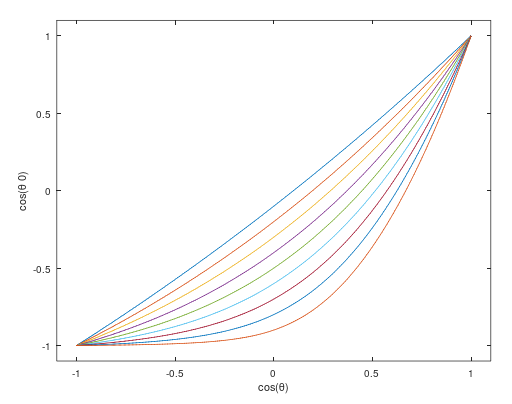
\includegraphics[width=10cm]{chapter_04_paragraph_16_fig_14a}
		\caption{\'Equation (\ref{EQ:16_6}) dans le cas $v_{0} > V$ pour $\dfrac{V}{v_{0}}$ compris entre 0.1 et 0.9 avec un pas de 0.1 et pour $0 < \theta < \pi$}\label{FIG:4_14A}
	\end{center}
\end{figure}

Dans le cas o\`u $v_{0} > V$, le vecteur $\vec{v}$ ne croise le cercle de rayon $v_{0}$ qu'en un unique point et comme il est n\'ecessaire de choisir $\theta_{0} = 0$ quand $\theta = 0$, la solution (\ref{EQ:16_6}) se r\'eduit \`a $\cos\theta_{0} = -\dfrac{V}{v_{0}}\sin^{2}\theta + \cos\theta\sqrt{1 - \dfrac{V^{2}}{v_{0}^{2}}\sin^{2}\theta}$. Ce cas est repr\'esent\'e sur la figure (\ref{FIG:4_14A}) Dans le cas o\`u $v_{0} < V$, le vecteur $\vec{v}$ croise le m\^eme cercle en deux points, B et C sur la figure correspondante (\ref{FIG:4_14}) tel qu'il existe alors deux valeurs de $\theta_{0}$ pour chaque valeur de $\theta$. Ce cas est illustr\'e sur la figure (\ref{FIG:4_14B}).

\begin{figure}[htb!]
	\begin{center}
		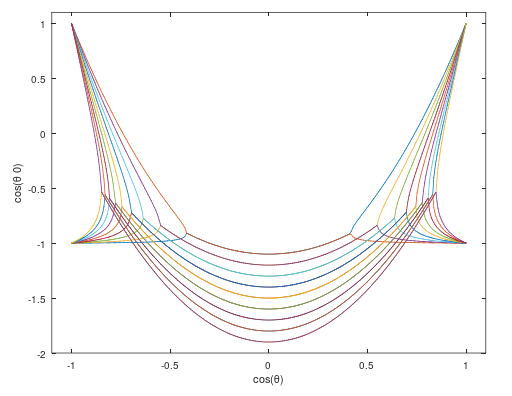
\includegraphics[width=10cm]{chapter_04_paragraph_16_fig_14b}
		\caption{Deux solutions de l'\'equation (\ref{EQ:16_6}) dans le cas $v_{0} < V$ pour $\dfrac{V}{v_{0}}$ compris entre 1.1 et 1.9 avec un pas de 0.1 et pour $0 < \theta < \pi$}\label{FIG:4_14B}
	\end{center}
\end{figure}

Dans la plupart des applications physiques, ce sont de nombreuses particules qui se d\'esint\`egrent et il faut alors raisonner en termes de distribution, en \'energie, en impulsion, en directions, etc. Prenons d\'esormais l'hypoth\`ese de particules initiales orient\'ees de mani\`ere chaotique, i.e. en moyenne de fa\c{c}on isotrope. Dans le r\'ef\'erentiel <<~c~>>, l'isotropie est conserv\'ee apr\`es les d\'esint\'egrations et les particules r\'esultantes de m\^eme esp\`ece ont alors la m\^eme \'energie et la r\'epartition des trajectoires est isotrope. L'orientation chaotique peut se traduire comme la quantit\'e de particules traversant un angle solide\footnote{Par d\'efinition, un \'el\'ement d'angle solide est d\'efini par $\mathrm{d}^{2}\Omega = \dfrac{\vec{r}\cdot\vec{n}}{r^{3}}\mathrm{d}^{2}S$ avec $\vec{r}$ le vecteur rayon et $\vec{n}$ le vecteur normale de l'\'el\'ement de surface $\mathrm{d}^{2}S$. Dans le cadre d'une sph\`ere, nous avons $\mathrm{d}^{2}S = r\mathrm{d}\theta r\sin\theta\mathrm{d}\varphi$ et par cons\'equent $\mathrm{d}^{2}\Omega = \sin\theta\mathrm{d}\theta\mathrm{d}\varphi$ ou encore $\mathrm{d}\Omega = 2\pi\sin\theta\mathrm{d}\theta$.} $\mathrm{d}\omega_{0}$ qui est proportionnelle \`a la grandeur de cet \'el\'ement soit $\frac{\mathrm{d}\omega_{0}}{4\pi}$. Dans le cadre d'une sph\`ere, $\mathrm{d}\omega_{0} = 2\pi\sin\theta_{0}\mathrm{d}\theta_{0}$, donc :
\be
	\dfrac{\mathrm{d}\omega_{0}}{4\pi} = \dfrac{1}{2}\sin\theta_{0}\mathrm{d}\theta_{0} \label{EQ:16_7}
\ee
Pour obtenir la r\'epartition dans le r\'ef\'erentiel <<~l~>>, partons du calcul de l'\'energie cin\'etique et de sa distribution. Nous savons que :
\bea
	\vec{v} & = & \vec{V} + \vec{v}_{0} \nonumber \\
	\Leftrightarrow v^{2} & = & v_{0}^{2} + V^{2} + 2v_{0}V\cos\theta_{0} \nonumber \\
	\Leftrightarrow \cos\theta_{0} & = & \dfrac{v^{2} - v_{0}^{2} - V^{2}}{2v_{0}V}
\eea
Or par rapport \`a $\theta_{0}$, les quantit\'es $\lVert\vec{v}_{0}\rVert$ et $\lVert\vec{V}\rVert$ sont constantes au contraire de $\lVert\vec{v}\rVert$ aussi, nous pouvons en conclure que :
\be
	\mathrm{d}\cos\theta_{0} = -\sin\theta_{0}\mathrm{d}\theta_{0} = \dfrac{\mathrm{d}(v^{2})}{2v_{0}V}
\ee
Or l'\'energie cin\'etique d'une particule r\'esultante de masse $m$ s\'ecrit $T = \frac{1}{2}mv^{2} \Leftrightarrow \mathrm{d}T = \frac{1}{2}m\mathrm{d}(v^{2})$. Donc en reprenant l'\'equation (\ref{EQ:16_7}) :
\bea
	\dfrac{\mathrm{d}\omega_{0}}{4\pi} & = & \dfrac{1}{2}\pi\sin\theta_{0}\mathrm{d}\theta_{0} = -\dfrac{\mathrm{d}(v^{2})}{4v_{0}V} \nonumber \\
	\Leftrightarrow \dfrac{\mathrm{d}\omega_{0}}{4\pi} & = & -\dfrac{\mathrm{d}(T)}{4mv_{0}V} \label{EQ:16_8}
\eea
En reprenant $v^{2} = v_{0}^{2} + V^{2} + 2v_{0}V\cos\theta_{0}$, nous en d\'eduisons que :
\begin{itemize}
	\item l'\'energie cin\'etique maximale est obtenue pour $\theta_{0} = 0$ et $T_{max} = \frac{m}{2}(v_{0} + V)^{2}$
	\item l'\'energie cin\'etique minimale est obtenue pour $\theta_{0} = \pi$ et $T_{max} = \frac{m}{2}(v_{0} - V)^{2}$
\end{itemize}
et dans cet intervalle, l'\'energie cin\'etique se distribue suivant la relation (\ref{EQ:16_8}).

Si la d\'esint\'egration donne plus de deux composantes, cela complexifie l'\'etude et en particulier, l'\'energie des composantes est loin d'\^etre unique dans le r\'ef\'erentiel <<~c~>>. Toutefois il existe une valeur maximale de l'\'energie cin\'etique pour chaque particule r\'esultante. Parmi l'ensemble des particules r\'esultants, consid\'erons-en une de masse $m_{1}$ et en posant $E_{int}'$, l'\'energie <<~interne~>> de l'ensemble des particules restantes moins $m_{1}$. Puisque cette situation permet de revenir \`a un probl\`eme \`a deux corps, la formule (\ref{EQ:16_1}) permet d'\'ecrire :
\be
	E_{int} = E_{int}' + T' + T_{10} + E_{1int}
\ee
avec $T'$ l'\'energie cin\'etique de l'ensemble des particules restantes moins $m_{1}$, $T_{10}$ l'\'energie cin\'etique de $m_{1}$ et $E_{1int}$ son \'energie interne. Les \'energies cin\'etiques peuvent s'\'ecrire avec $M$ la masse de la particule initiale :
\be
	T' = \dfrac{p_{0}^{2}}{2(M - m_{1})}\text{ et }T_{10} = \dfrac{p_{0}^{2}}{2m_{1}}
\ee
donc :
\bea
	E_{int} - E_{int}' - E_{1int} & = & \dfrac{M}{M - m_{1}}\dfrac{p_{0}^{2}}{2m_{1}} \nonumber \\
	\Leftrightarrow T_{10} & = & \dfrac{M - m_{1}}{M}(E_{int} - E_{int}' - E_{1int})
\eea
Aussi $T_{10}$ est maximale si et seulement si $E_{int}'$ est minimale. Ceci intervient lorsque toutes les particules r\'esultantes, sauf $m_{1}$, ont la m\^eme vitesse, i.e. une agitation du syst\`eme minimale et $E_{int}'$ devient simplement la somme des \'energies internes de cet ensemble de particules. Dans ce cas pr\'ecis, la quantit\'e $E_{int} - E_{int}' - E_{1int}$ repr\'esente $\epsilon$, l'\'energie de d\'esint\'egration d\'efinie dans l'\'equation (\ref{EQ:16_2}). Nous en concluons :
\be
	T_{10max} = \dfrac{M - m_{1}}{M}\epsilon \label{EQ:16_9}
\ee

\section{Chocs \'elastiques des particules}

Le choc entre deux particules est dit \'elastique lorsqu'il n'y a pas de modifications de leur \'etat interne. Lors de l'application de la loi de conservation de l'\'energie, il n'est donc pas n\'ecessaire de prendre en compte les \'energies internes respectives. Dans le r\'ef\'erentiel du centre d'inertie <<~c~>>, ce dernier est de facto au repos. Avant le choc, par application de la conservation de l'impulsion, nous avons dans <<~c~>> : $m_{1}\vec{v}_{10} + m_{2}\vec{v}_{20} = \vec{0}$. Dans <<~l~>>, la position du centre d'inertie s'\'ecrit :
\be
	\vec{R} = \dfrac{m_{1}\vec{r}_{1} + m_{2}\vec{r}_{2}}{m_{1} + m_{2}}
\ee
et la loi de composition des vitesses am\`ene \`a \'ecrire :
\be
	\begin{cases}
		\vec{v}_{1} = \vec{v}_{10} + \frac{\mathrm{d}\vec{R}}{\mathrm{dt}} \\
		\vec{v}_{2} = \vec{v}_{20} + \frac{\mathrm{d}\vec{R}}{\mathrm{dt}}
	\end{cases}
\ee
donc en soustrayant les deux relations et en d\'efinissant\footnote{Voir une \'equivalence avec les relations (\ref{EQ:13_2})} $\vec{v} = \vec{v}_{1} - \vec{v}_{2}$ :
\be
	\vec{v} = \vec{v}_{10} - \vec{v}_{20}
\ee
En reprenant la conservation de l'impulsion dans <<~c~>>, nous avons alors :
\be
	\begin{cases}
		\vec{v} = \vec{v}_{10} + \frac{m_{1}}{m_{2}}\vec{v}_{10} \Leftrightarrow \vec{v}_{10} = \frac{m_{2}}{m_{1} + m_{2}}\vec{v} \\
		\vec{v} = -\vec{v}_{20} - \frac{m_{2}}{m_{1}}\vec{v}_{20} \Leftrightarrow \vec{v}_{20} = -\frac{m_{1}}{m_{1} + m_{2}}\vec{v}
	\end{cases}
\ee

Comme le choc est \'elastique, dans <<~c~>>, la conservation de l'impulsion après le choc donne $m_{1}\vec{v'}_{10} + m_{2}\vec{v'}_{20} = \vec{0}$ et comme avant le choc, nous avons $m_{1}\vec{v}_{10} + m_{2}\vec{v}_{20} = \vec{0}$, nous pouvons en conclure que c'est vrai si $m_{1}(\vec{v'}_{10} + \vec{v}_{10}) + m_{2}(\vec{v'}_{20} + \vec{v}_{20}) = \vec{0}$, soit $\vec{v'}_{10} = -\vec{v}_{10}$ et $\vec{v'}_{20} = -\vec{v}_{20}$. De m\^eme, la conservation de l'\'energie avant et apr\`es le choc, et qui ne concerne que les \'energies cin\'etiques, implique que l'\'energie de chacune des deux particules est conserv\'ees car $v'_{10} = v_{10}$ et $v'_{20} = v_{20}$.
Par cons\'equent, dans <<~c~>>, l'unique diff\'erence entre avant et apr\`es le choc se situe dans l'inversion de la direction de la vitesse de chacune des deux particules.

D\'efinissons le vecteur unitaire $\vec{n}_{0}$ dans la direction de la vitesse apr\`es le choc de la particule de masse $m_{1}$. Alors $\vec{v'}_{10} = v'_{10}\vec{n}_{0} = v_{10}\vec{n}_{0}$. Le vecteur $\vec{n}_{0}$ absorbe l'inversion de direction apr\`es le choc et permet de reprendre les relations ci-dessous pour en conclure :
\be
	\begin{cases}
		\vec{v'}_{10} = \frac{m_{2}}{m_{1} + m_{2}}v\vec{n}_{0} \\
		\vec{v'}_{20} = -\frac{m_{1}}{m_{1} + m_{2}}v\vec{n}_{0} \label{EQ:17_1}
	\end{cases}
\ee
Le passage de <<~c~>> \`a <<~l~>> via la loi de composition des vitesses et l'expression de la vitesse du centre d'inertie dans <<~l~>> permet d'\'ecrire :
\be
	\begin{cases}
		\vec{v'}_{1} = \vec{v'}_{10} + \frac{\mathrm{d}\vec{R'}}{\mathrm{dt}} \\
		\vec{v'}_{2} = \vec{v'}_{20} + \frac{\mathrm{d}\vec{R'}}{\mathrm{dt}}
	\end{cases}
\ee
avec :
\be
	\dfrac{\mathrm{d}\vec{R'}}{\mathrm{dt}} = \dfrac{m_{1}\vec{v'}_{1} + m_{2}\vec{v'}_{2}}{m_{1} + m_{2}} = \dfrac{m_{1}\vec{v}_{1} + m_{2}\vec{v}_{2}}{m_{1} + m_{2}}
\ee
par l'additivit\'e des int\'egrales du mouvement, voir le paragraphe (\ref{PAR:6}) qui implique que les lois de conservation ne d\'ependent pas des interactions en jeu, en particulier pour celle de l'impulsion ici. Par cons\'equent, en reportant les \'equations (\ref{EQ:17_1}) :
\be
	\begin{cases}
		\vec{v'}_{1} = \frac{m_{2}}{m_{1} + m_{2}}v\vec{n}_{0} + \frac{m_{1}\vec{v}_{1} + m_{2}\vec{v}_{2}}{m_{1} + m_{2}} \\
		\vec{v'}_{2} = -\frac{m_{1}}{m_{1} + m_{2}}v\vec{n}_{0} + \frac{m_{1}\vec{v}_{1} + m_{2}\vec{v}_{2}}{m_{1} + m_{2}} \label{EQ:17_2}
	\end{cases}
\ee
o\`u seul le vecteur $\vec{n}_{0}$ est une cons\'equence de la loi d'interaction entre les particules. En multipliant les relations (\ref{EQ:17_2}) par la masse respective des particules, nous arrivons \`a exprimer leur impulsion apr\`es le choc en fonction de celle avant le choc, le tout dans le r\'ef\'erentiel <<~l~>> :
\be
	\begin{cases}
		\vec{p'}_{1} = mv\vec{n}_{0} + \frac{m_{1}}{m_{1} + m_{2}}(\vec{p}_{1} + \vec{p}_{2}) \\
		\vec{p'}_{2} = -mv\vec{n}_{0} + \frac{m_{2}}{m_{1} + m_{2}}(\vec{p}_{1} + \vec{p}_{2}) \label{EQ:17_3}
	\end{cases}
\ee
avec $m$ la masse r\'eduite du syt\`eme d\'efinie telle que $m = \frac{m_{1}m_{2}}{m_{1} + m_{2}}$.

\begin{figure}[htb!]
	\begin{center}
		\begin{picture}(300,300)(0,0)
			%circle
			\linethickness{0.05mm}
			\put(150,150){\circle{200}}
			%vectors circle
			\linethickness{0.5mm}
			\put(60,150){\vector(1,0){90}}
			\put(150,150){\vector(1,0){50}}
			\put(60,150){\vector(7,6){115}}\put(90,190){$\vec{p'}_{1}$}
			\put(150,150){\vector(1,5){20}}\put(160,185){$\vec{n}_{0}$}
			\put(170,246){\vector(3,-10){29}}\put(195,190){$\vec{p'}_{2}$}
			%points circle
			\put(146,138){$O$}
			\put(51,148){$A$}
			\put(202,146){$B$}
			\put(175,250){$C$}
		\end{picture}
		\caption{Repr\'esentation g\'eom\'etrique d'un choc entre deux particules}\label{FIG:4_15}
	\end{center}
\end{figure}

Sur la figure (\ref{FIG:4_15}) est trac\'e le cercle de rayon $mv$. Les vecteurs $\vec{AC}$ et $\vec{CB}$ donnent respectivement $\vec{p'}_{1}$ et $\vec{p'}_{2}$ en accord avec les relations (\ref{EQ:17_3}). Les impulsions initiales $\vec{p}_{1}$ et $\vec{p}_{2}$ impliquent que les points $A$ et $B$ ne changent pas de position, aussi seul le point $C$ peut avoir une position quelconque sur le cercle de rayon $mv$. Par construction g\'eom\'etrique, les relations (\ref{EQ:17_3}) donnent :
\be
	\begin{cases}
		\vec{AO} = \frac{m_{1}}{m_{1} + m_{2}}(\vec{p}_{1} + \vec{p}_{2}) \\
		\vec{OB} = \frac{m_{2}}{m_{1} + m_{2}}(\vec{p}_{1} + \vec{p}_{2})
	\end{cases}
\ee

\subsection{Cas de la particule $m_{2}$ au repos avant le choc}

\begin{figure}[htb!]
	\begin{center}
		\begin{picture}(500,300)(0,0)
			%circles
			\linethickness{0.05mm}
			\put(100,150){\circle{200}}\put(90,25){$m_{1} < m_{2}$}
			\put(400,150){\circle{200}}\put(390,25){$m_{1} > m_{2}$}
			%vectors circle #1
			\linethickness{0.5mm}
			\put(40,150){\vector(1,0){160}}
			\put(40,150){\vector(9,5){130}}\put(90,190){$\vec{p'}_{1}$}
			\put(169,221){\vector(3,-7){32}}\put(165,180){$\vec{p'}_{2}$}
			%angles circle #1
			\linethickness{0.05mm}
			\multiput(100,150)(10,10){7}{\line(1,1){8}}
			\qbezier(55,150)(55,155)(50,155)\put(60,153){$\theta_{1}$}
			\qbezier(110,150)(110,155)(105,155)\put(114,154){$\xi$}
			\qbezier(180,150)(188,165)(194,165)\put(170,155){$\theta_{2}$}
			%points circle #1
			\put(95,135){$O$}
			\put(30,147){$A$}
			\put(202,147){$B$}
			\put(175,220){$C$}
			%vectors circle #2
			\linethickness{0.5mm}
			\put(250,150){\vector(1,0){250}}
			\put(250,150){\vector(10,3){220}}\put(390,200){$\vec{p'}_{1}$}
			\put(469,221){\vector(3,-7){32}}\put(465,180){$\vec{p'}_{2}$}
			%\theta_{max} case
			\linethickness{0.05mm}
			\put(250,150){\line(10,9){90}}
			\put(400,150){\line(-11,15){60}}
			%angles circle #2
			\linethickness{0.05mm}
			\multiput(400,150)(10,10){7}{\line(1,1){8}}
			\qbezier(280,150)(280,158)(275,158)\put(287,152){$\theta_{1}$}
			\qbezier(410,150)(410,155)(405,155)\put(412,153){$\xi$}
			\qbezier(480,150)(488,165)(494,165)\put(470,155){$\theta_{2}$}
			\qbezier(320,150)(320,190)(294,190)\put(315,182){$\theta_{max}$}
			%points circle #2
			\put(395,135){$O$}
			\put(240,147){$A$}
			\put(502,147){$B$}
			\put(475,220){$C$}
		\end{picture}
		\caption{Repr\'esentation g\'eom\'etrique de d\'esint\'egrations dans le cas $\vec{v}_{2} = \vec{0}$}\label{FIG:4_16}
	\end{center}
\end{figure}

Si la particule de masse $m_{2}$ est au repos avant le choc, cela se traduit par $v_{2} = \vec{0} = p_{2}$. Nous avons aussi :
\be
	\vec{OB} = \dfrac{m_{2}}{m_{1} + m_{2}}(\vec{p}_{1} + \vec{p}_{2}) = \frac{m_{1}m_{2}}{m_{1} + m_{2}}\vec{v}_{1} = m\vec{v}_{1} = m\vec{v}
\ee
car par d\'efinition, $\vec{v} = \vec{v}_{1} - \vec{v}_{2}$ et donc \'egal \`a $\vec{v}_{1}$ dans le cas qui nous occupe. Donc le point $B$ se trouve positionner sur le cercle de rayon $mv$. De plus :
\be
	\vec{AB} = \vec{AO} + \vec{OB} = \frac{m_{1}}{m_{1} + m_{2}}\vec{p}_{1} + \dfrac{m_{2}}{m_{1} + m_{2}}\vec{p}_{1} = \vec{p}_{1}
\ee
Le vecteur $\vec{AB}$ repr\'esente donc l'impulsion de d\'epart de la particule de masse $m_{1}$.

Les points $A$, $O$ et $B$ se situant sur la m\^eme droite, nous pouvons en d\'eduire :
\be
	AO = AB - OB = m_{1}v_{1} - \dfrac{m_{1}m_{2}}{m_{1} + m_{2}}v_{1} = \dfrac{m_{1}^{2}}{m_{1} + m_{2}}v_{1} = \dfrac{m_{1}}{m_{2}}OB
\ee
Par cons\'equent :
\begin{itemize}
	\item si $m_{1} < m_{2}$ alors le point $A$ se situe \`a l'int\'erieur du cercle
	\item si $m_{1} = m_{2}$ alors le point $A$ se situe sur le cercle
	\item si $m_{1} > m_{2}$ alors le point $A$ se situe \`a l'ext\'erieur du cercle
\end{itemize}
Ces cas sont repr\'esent\'es sur la figure (\ref{FIG:4_16}). Sur celle-ci, les angles $\theta_{1}$ et $\theta_{2}$ sont les angles de d\'eviation dans <<~l~>> par rapport \`a la direction du choc, d\'efinie par $\vec{p}_{1}$ et $\xi$ est l'angle de d\'eviation de la particule de masse $m_{1}$ dans <<~c~>>. Les angles $\theta_{1}$ et $\theta_{2}$ peuvent \^etre calcul\'es ainsi :
\be
	\begin{cases}
		\tan\theta_{1} = \dfrac{mv\sin\xi}{AO + mv\cos\xi} = \dfrac{\dfrac{m_{1}m_{2}}{m_{1} + m_{2}}v\sin\xi}{\dfrac{m_{1}^{2}}{m_{1} + m_{2}}v + \dfrac{m_{1}m_{2}}{m_{1} + m_{2}}v\cos\xi} = \dfrac{m_{2}\sin\xi}{m_{1} + m_{2}\cos\xi} \\
		\\
		\pi = \dfrac{\pi}{2} + \dfrac{\xi}{2} + \theta_{2} \Leftrightarrow \theta_{2} = \dfrac{\pi - \xi}{2} \label{EQ:17_4}
	\end{cases}
\ee

D\'eterminons ensuite la valeur de la vitesse apr\`es le choc pour les deux particules dans <<~l~>>. Nous avons d\'ej\`a vu que $\vec{v'}_{1} = \vec{v'}_{10} + \vec{\dot{R'}}$ sachant que $\vec{\dot{R'}} = \vec{\dot{R}}$, aussi :
\be
	{v'}_{1}^{\,2} = {v'}_{10}^{\,2} + {\lVert \vec{\dot{R}} \rVert}^{2} + 2v'_{10}\lVert \vec{\dot{R}} \rVert\cos\theta_{10}
\ee
or $\theta_{10} = \xi$ par d\'efinition, donc :
\be
	{v'}_{1}^{\,2} = \dfrac{m_{2}^{2}}{(m_{1} + m_{2})^{2}}v^{2} + \dfrac{m_{1}^{2}}{(m_{1} + m_{2})^{2}}v_{1}^{2} + 2\dfrac{m_{1}m_{2}}{(m_{1} + m_{2})^{2}}vv_{1}\cos\xi
\ee
et comme $v_{1} = v$, nous avons :
\be
	v'_{1} = \dfrac{\sqrt{m_{1}^{2} + m_{2}^{2} + 2m_{1}m_{2}\cos\xi}}{m_{1} + m_{2}}v \label{EQ:17_5A}
\ee
De mani\`ere similaire pour $v'_{2}$, nous avons $\vec{v'}_{1} = \vec{v'}_{10} + \vec{\dot{R}}$, soit :
\bea
	{v'}_{2}^{\,2} & = & {v'}_{20}^{\,2} + {\lVert \vec{\dot{R}} \rVert}^{2} + 2v'_{20}\lVert \vec{\dot{R}} \rVert\cos(\langle \vec{v'}_{20},\vec{\dot{R}} \rangle) \nonumber \\
	& = & \dfrac{m_{1}^{2}}{(m_{1} + m_{2})^{2}}v^{2} + \dfrac{m_{1}^{2}}{(m_{1} + m_{2})^{2}}v_{1}^{2} + 2\dfrac{m_{1}^{2}}{(m_{1} + m_{2})^{2}}vv_{1}\cos\theta_{20}
\eea
et comme $v_{1} = v$ et $\theta_{20} = \pi - \xi$ :
\bea
	{v'}_{2}^{\,2} & = &  2\dfrac{m_{1}^{2}}{(m_{1} + m_{2})^{2}}v^{2} - 2\dfrac{m_{1}^{2}}{(m_{1} + m_{2})^{2}}v^{2}\cos\xi \nonumber \\
	& = & 2\dfrac{m_{1}^{2}}{(m_{1} + m_{2})^{2}}v^{2}(1 - \cos\xi) = 2\dfrac{m_{1}^{2}}{(m_{1} + m_{2})^{2}}v^{2}\left(1 - 1 + 2\sin^{2}\left(\dfrac{\xi}{2}\right)\right) \nonumber \\
	& = & 4\dfrac{m_{1}^{2}}{(m_{1} + m_{2})^{2}}v^{2}\sin^{2}\left(\dfrac{\xi}{2}\right)
\eea
car :
\be
	\cos\xi = \cos\left(\dfrac{\xi}{2} + \dfrac{\xi}{2}\right) = \cos^{2}\left(\dfrac{\xi}{2}\right) - \sin^{2}\left(\dfrac{\xi}{2}\right) = 1 - 2\sin^{2}\left(\dfrac{\xi}{2}\right)
\ee
Nous arrivons donc \`a :
\be
	v'_{2} = \dfrac{m_{1}}{m_{1} + m_{2}}v\sin\left(\dfrac{\xi}{2}\right) \label{EQ:17_5B}
\ee

\subsection{Cas d'un choc entre deux particules de même masse dont l'une au repos avant le choc}

\begin{figure}[htb!]
	\begin{center}
		\begin{picture}(300,300)(0,0)
			%circles
			\linethickness{0.05mm}
			\put(150,150){\circle{200}}
			%vectors circle #1
			\linethickness{0.5mm}
			\put(50,150){\vector(1,0){200}}
			\put(50,150){\vector(9,4){170}}\put(140,200){$\vec{p'}_{1}$}
			\put(219,221){\vector(3,-7){32}}\put(215,180){$\vec{p'}_{2}$}
			%angles circle #1
			\linethickness{0.05mm}
			\multiput(150,150)(10,10){7}{\line(1,1){8}}
			\qbezier(65,150)(65,155)(60,155)\put(75,153){$\theta_{1}$}
			\qbezier(160,150)(160,155)(155,155)\put(164,154){$\xi$}
			\qbezier(230,150)(238,165)(244,165)\put(220,155){$\theta_{2}$}
			%points circle #1
			\put(145,135){$O$}
			\put(40,147){$A$}
			\put(252,147){$B$}
			\put(225,220){$C$}
		\end{picture}
		\caption{Repr\'esentation g\'eom\'etrique de d\'esint\'egrations dans le cas $\vec{v}_{2} = \vec{0}$ et $m_{1} = m_{2}$}\label{FIG:4_17}
	\end{center}
\end{figure}
\chapter{Petites oscillations}

\section{Oscillations lin\'eaires libres}\label{PAR:21}

Les \emph{petites oscillations} sont celles faites par un syst\`eme au voisinage de sa position d'\'equilibre stable et nous étudions ici le cas le plus simple, celui où il n'y a qu'un seul degr\'e de libert\'e. Un \'equilibre stable intervient quand l'\'energie potentielle $U(q)$ est minimale. D\'efinissons que $U$ soit minimale en $q = q_{0}$. L'\'equation (\ref{EQ:5_4}) montre qu'un \'ecart par rapport \`a la position $q_{0}$ engendre une force \'egale \`a $-\frac{\mathrm{d}U}{\mathrm{d}q}$ qui ram\`ene le syst\`eme \`a sa position d'\'equilibre stable. R\'ealisons un d\'eveloppement de Taylor de $U(q)$ jusqu'au second ordre :
\benn
	U(q) = U(q_{0}) + U'(q_{0})(q - q_{0}) + \dfrac{U''(q_{0})}{2}(q - q_{0})^{2} \Rightarrow U(q) - U(q_{0}) = \dfrac{k}{2}(q - q_{0})^{2}
\eenn
car $U'(q_{0}) = 0$ puisque $q_{0}$ est la position d'\'equilibre et nous avons pos\'e $k = U''(q_{0})$. En d\'efinissant :
\be
	x = q - q_{0} \label{EQ:21_1}
\ee
qui repr\'esente l'\'ecart par rapport \`a la position d'\'equilibre, nous avons, en posant $U(q_{0}) = 0$ :
\be
	U(x) = \dfrac{kx^{2}}{2} \label{EQ:21_2}
\ee
Au regard des relations (\ref{EQ:4_1}) et (\ref{EQ:5_5}), l'\'energie cin\'etique pour une particule et dans le cas d'un unique degr\'e de libert\'e, s'\'ecrit $T = \frac{1}{2}a(q)\dot{q}^{2}$. Or dans le cadre des petites oscillations, $x \approx q$. De la m\^eme mani\`ere, $a(q) \approx q(a_{0})$, quantit\'e qui peut s'identifier \`a la masse de la particule si $x$ est une coordonn\'ee cart\'esienne. L'\'energie cin\'etique peut donc se formuler comme $T = \frac{1}{2}m\dot{x}^{2}$. Par cons\'equent, la fonction de Lagrange pour un syst\`eme r\'ealisant de petites oscillations, d\'enomm\'e aussi \emph{oscillateur lin\'eaire} est :
\be
	L = \dfrac{m\dot{x}^{2}}{2} - \dfrac{kx^{2}}{2} \label{EQ:21_3}
\ee
Dans notre cas \'epur\'e, l'\'equation du mouvement s'obtient \`a partir de la relation (\ref{EQ:5_2}) :
\be
	\dfrac{\mathrm{d}}{\mathrm{dt}}\left(\dfrac{\partial L}{\partial \dot{x}}\right) = \dfrac{\partial L}{\partial x} \Leftrightarrow \dfrac{\mathrm{d}m\dot{x}}{\mathrm{dt}} = -kx \Leftrightarrow m\ddot{x} + kx = 0 \label{EQ:21_4}
\ee
\'Equation qui peut \'egalement s'\'ecrire :
\be
	\ddot{x} + \omega^{2}x = 0 \label{EQ:21_5}
\ee
en posant la quantit\'e :
\be
	\omega = \sqrt{\dfrac{k}{m}} \label{EQ:21_6}
\ee
qui est appel\'ee \emph{fr\'equence angulaire}. La quantit\'e $\omega$ ne d\'epend pas des conditions initiales du mouvement mais uniquement des propri\'et\'es m\'ecaniques du syst\`eme, c'est une constante fondamentale des oscillations. Ceci n'est valable que dans le cas qui nous concerne, celui des petites oscillations, ou encore quand $U \propto x^{2}$. Pour les cas g\'en\'eraux, nous pouvons nous reporter \`a l'\'equation (\ref{EQ:11_EX2A_1}) qui d\'efinit la p\'eriode d'oscillations $T$ pour $U = A\lvert x^{n} \rvert$, sachant que $\omega = 2\pi/T$.

L'\'equation (\ref{EQ:21_5} admet deux solutions ind\'ependantes en $\cos(\omega t)$ et en $\sin(\omega t)$. Donc la solution g\'en\'erale s'\'ecrit :
\be
	x = c_{1}\cos(\omega t) + c_{2}\sin(\omega t) \label{EQ:21_7}
\ee
ou encore :
\be
	x = a\cos(\omega t + \alpha) \label{EQ:21_8}
\ee
o\`u $a$ est l'\emph{amplitude} et $\alpha$ la valeur initiale de la \emph{phase}, qui d\'epend de l'origine prise pour $t$.Comme $\cos(\omega t + \alpha) = \cos(\omega t)\cos\alpha - \sin(\omega t)\sin\alpha$, alors nous pouvons en d\'eduire, \`a partir de la relation (\ref{EQ:21_7}), $c_{1} = a\cos\alpha$ et $c_{2} = -a\sin\alpha$. De plus :
\be
	\begin{cases}
		c_{1}^{2} + c_{2}^{2} = a^{2}(\cos^{2}\alpha + \sin^{2}\alpha) \Rightarrow a = \sqrt{c_{1}^{2} + c_{2}^{2}} \\
		\dfrac{\sin\alpha}{\cos\alpha} = \tan\alpha = -\dfrac{c_{2}}{c_{1}} \label{EQ:21_9}
	\end{cases}
\ee
L'\'energie totale du syst\`eme vaut, en y ajoutant la formule (\ref{EQ:21_8}) :
\bea
	E & = & T + U = \dfrac{m\dot{x}^{2}}{2} + \dfrac{kx^{2}}{2} = \dfrac{m}{2}(\dot{x}^{2} + \omega^{2}x^{2}) \nonumber \\
	& = & \dfrac{m}{2}(a^{2}\omega^{2}\sin^{2}(\omega t + \alpha) + a^{2}\omega^{2}\cos^{2}(\omega t + \alpha)) = \dfrac{m\omega^{2}a^{2}}{2} \label{EQ:21_10}
\eea
Il est souvent ais\'e de passer dans le domaine complexe pour simplifier les op\'erations math\'ematiques et de consid\'erer la solution (\ref{EQ:21_8}) comme :
\be
	x = \Re{\{Ae^{i\omega t}\}} \label{EQ:21_11}
\ee
avec l'\emph{amplitude complexe} s'exprimant comme :
\be
	A = ae^{i\alpha} \label{EQ:21_12}
\ee
dont le module est l'amplitude ordinaire et l'argument la phase initiale.

\section{Oscillations forc\'ees}\label{PAR:22}

Les \emph{oscillations forc\'ees} sont les oscillations d'un syst\`eme soumis \`a un champ ext\'erieur variable. En restant dans l'hypoth\`ese des petites oscillations, cela implique que le champ ext\'erieur est suffisamment faible pour provoquer des d\'eplacements faibles \'egalement. De plus, ici, nous restons dans le cadre d'un unique degr\'e de libert\'e.

\subsection{Cas g\'en\'eral}

L'\'energie potentielle totale du syst\`eme s'\'ecrit avec deux termes, \`a savoir l'\'energie potentielle propre en $\frac{1}{2}kx^{2}$ et celle due \`a l'action ext\'erieur $U_{e}(x,t)$. Au premire ordre, cette derni\`ere s'\'ecrit :
\benn
	U_{e}(x,t) = U_{e}(0,t) + x\left(\dfrac{\partial U_{e}}{\partial x}\right)(0,t)
\eenn
o\`u $U_{e}(0,t)$ est une fonction ne d\'ependant que du temps et de facto, elle est le r\'esultat d'une d\'eriv\'ee totale par rapport au temps. Dans cette partie est n\'eglig\'ee dans l'\'equation de Lagrange, voir (\ref{EQ:2_8}). De plus, la formule (\ref{EQ:5_8}) permet de d\'eduire que $-\frac{\partial U_{e}}{\partial x}$ est la force ext\'erieure qui s'exerce sur le syst\`eme. Elle est fonction du temps et nous la d\'esignons $F(t)$. Par cons\'equent, $U_{e}(x,t) = -xF(t)$ et la fonction de Lagrange peut se formuler ainsi :
\be
	L = \dfrac{m}{2}\dot{x}^{2} - \left(\frac{k}{2}x^{2} - xF(t)\right) \label{EQ:22_1}
\ee
L'\'equation du mouvement provenant de la formule (\ref{EQ:5_2}) permet d'en d\'eduite :
\bea
	\dfrac{\mathrm{d}}{\mathrm{dt}}\left(\dfrac{\partial L}{\partial \dot{x}}\right) & = & \dfrac{\partial L}{\partial x} \Leftrightarrow \dfrac{\mathrm{d}m\dot{x}}{\mathrm{dt}} = -kx + F(t) + x\dfrac{\partial F(t)}{\partial x} \nonumber \\
	& \Leftrightarrow & m\ddot{x} + kx = F(t) \Leftrightarrow \ddot{x} + \omega^{2}x = \dfrac{F(t)}{m} \label{EQ:22_2}
\eea
avec $\omega = \sqrt{\frac{k}{m}}$ la fr\'equence des oscillations. L'\'equation (\ref{EQ:22_2}) est une \'equation diff\'erentielle du second ordre avec des c{\oe}fficients constants et un second membre. La solution g\'en\'erale est de la forme $x = x_{0} + x_{1}$ telle que :
\begin{itemize}
	\item $x_{0}$ est la solution g\'en\'erale de l'\'equation sans second membre qui repr\'esente les oscillations libres d\'etermin\'ee aux \'equations (\ref{EQ:21_7}) et (\ref{EQ:21_8})
	\item $x_{1}$ est une int\'egrale particuli\`ere de l'\'equation avec le second membre
\end{itemize}

\subsection{Cas particulier d'une force ext\'erieure p\'eriodique}

Consid\'erons que la force ext\'erieure s'exprime telle que :
\be
	F(t) = f\cos(\gamma t + \beta) \label{EQ:22_3}
\ee
Pour cette hypoth\`ese, l'int\'egrale particuli\`ere de l'\'equation (\ref{EQ:22_2}) peut \^etre $x_{1} = b\cos(\gamma t + \beta)$, ce qui nous donne :
\bea
	& & -b\gamma^{2}\cos(\gamma t + \beta) + \omega^{2}b\cos(\gamma t + \beta) = \dfrac{f}{m}\cos(\gamma t + \beta) \Leftrightarrow b(\omega^{2} - \gamma^{2}) = \dfrac{f}{m} \nonumber \\
	& \Leftrightarrow & b = \dfrac{f}{m(\omega^{2} - \gamma^{2})} \nonumber
\eea
Le mouvement se compose donc en ajoutant la solution g\'en\'erale (\ref{EQ:21_8}) :
\be
	x = a\cos(\omega t + \alpha) + \frac{f}{m(\omega^{2} - \gamma^{2})}\cos(\gamma t + \beta) \label{EQ:22_4}
\ee
o\`u les quantit\'es $a$ et $\alpha$ sont d\'eduites des conditions initiales. Le mouvement est ainsi compos\'e de la somme de deux oscillations, la premi\`ere avec la fr\'equence propre du syst\`eme et la seconde avec la fr\'equence de la force ext\'erieure. La formule (\ref{EQ:22_4}) est ind\'etermin\'ee dans le cas o\`u $\omega = \gamma$, il y a alors \emph{r\'esonnance}.

\subsection{Solution r\'eelle lors de la r\'esonnance avec une force ext\'erieure}

Partons de la formule (\ref{EQ:22_4}) pour la reformuler ainsi :
\benn
	x = a\cos(\omega t + \alpha) + \frac{f}{m(\omega^{2} - \gamma^{2})}(\cos(\gamma t + \beta) - \cos(\omega t + \beta))
\eenn
Ainsi lorsque $\gamma \rightarrow \omega$, alors nous avons une ind\'etermination de type $0/0$ pour le second terme. Appliquons alors la r\`egle de L'Hospital\footnote{Si $f$ et $g$ sont deux fonctions d\'efinies sur $[a;b[$, d\'erivables en $a$ et telles que $f(a) = g(a) = 0$ et $g'(a) \neq 0$ alors $\lim_{x \rightarrow a^{+}}\dfrac{f(x)}{g(x)} = \dfrac{f'(a)}{g'(a)}$} avec :
\benn
	\begin{cases}
		f : \omega \mapsto \cos(\gamma t + \beta) - \cos(\omega t + \beta) \\
		g : \omega \mapsto w^{2} - \gamma^{2}
	\end{cases}
\eenn
Cela nous donne :
\benn
	\lim_{\gamma \rightarrow \omega}\dfrac{f(\gamma)}{g(\gamma)} = \dfrac{f'(\gamma = \omega)}{g'(\gamma = \omega)} = \dfrac{-t\sin(\omega t + \beta)}{-2\omega}
\eenn
et nous permet d'\'ecrire :
\be
	x = a\cos(\omega t + \alpha) + \frac{f}{2m\omega}t\sin(\omega t + \beta) \label{EQ:22_5}
\ee
Dans le cas de la r\'esonnance, l'amplitude augmente lin\'eairement avec le temps tant que nous restons dans le cadre des petites oscillations.

\subsection{Solution complexe lors de la r\'esonnance avec une force ext\'erieure}

Au voisinage de la r\'esonnance, d\'efinissons la fr\'equence $\gamma = \omega + \epsilon$ avec $\epsilon$ petit devant $\omega$. Dans le domaine complexe, il est possible de g\'en\'eraliser l'expression (\ref{EQ:22_4}) telle que :
\be
	x = Ae^{i\omega t} + Be^{i(\omega + \epsilon)t} = \left(A + Be^{i\epsilon t}\right)e^{i\omega t} \label{EQ:22_6}
\ee
Comme $\epsilon \ll \omega$, l'expression $A + Be^{i\epsilon t}$ varie peu lors d'une p\'eriode $2pi/\omega$. Au voisinage de la r\'esonnance, le mouvement se constitue de petites oscillations \`a amplitude variable. L'amplitude reste une grandeure r\'eelle aussi nous d\'efinissons $C = \lvert A + Be^{i\epsilon t} \lvert$. La relation (\ref{EQ:21_12}) permet d'\'ecrire $A = ae^{i\alpha}$ et $B = be^{i\beta}$, et ainsi l'amplitude $C$ devient :
\bea
	C & = & \lvert ae^{i\alpha} + be^{i(\epsilon t + \beta)} \rvert \nonumber \\
	\Leftrightarrow C^{2} & = & \lvert ae^{i\alpha} \rvert^{2} + \lvert be^{i(\epsilon t + \beta)} \rvert^{2} + 2\lvert ae^{i\alpha} \rvert \cdot \lvert be^{i(\epsilon t + \beta)} \rvert \cos(\epsilon t + \beta - \alpha) \nonumber \\
	C^{2} & = & a^{2} + b^{2} + 2ab\cos(\epsilon t + \beta - \alpha) \label{EQ:22_7}
\eea
Les valeurs extremum de $C$ sont :
\begin{itemize}
	\item $C_{max}^{2} = a^{2} + b^{2} + 2ab \Rightarrow C_{max} = a + b$
	\item $C_{min}^{2} = a^{2} + b^{2} - 2ab \Rightarrow C_{min} = \lvert a - b \rvert$
\end{itemize}
Par cons\'equent, l'amplitude $C$ oscille p\'eriodiquement entre les deux valeurs pr\'ec\'edentes avec une fr\'equence $\epsilon$, ph\'enom\`ene appel\'e \emph{battements}.

Ensuite, nous pouvons remarquer que l'\'equation (\ref{EQ:22_2}) peut s\'ecrire :
\bea
	\ddot{x} + i\omega\dot{x} - i\omega\dot{x} - i\omega\cdot i\omega x & = & \dfrac{F(t)}{m} \Leftrightarrow \dfrac{\mathrm{d}}{\mathrm{dt}}(\dot{x} + i\omega x) - i\omega(\dot{x} + i\omega x) = \dfrac{F(t)}{m} \nonumber \\
	\Rightarrow \dfrac{\mathrm{d}\xi}{\mathrm{dt}} - i\omega\xi = \dfrac{F(t)}{m} \label{EQ:22_8}
\eea
en d\'efinissant la quantit\'e $\xi$ telle que :
\be
	\xi = \dot{x} + i\omega x \label{EQ:22_9}
\ee
L'\'equation (\ref{EQ:22_8}) n'est plus du second ordre. Sa solution g\'en\'erale sans second membre peut d'\'ecrire comme $\xi_{0}e^{i\omega t}$ avec $\xi_{0}$ une constante d\'ependant des conditions initialies et \'egale \`a $\xi(t=0)$. Cherchons d\'esormais un int\'egrale particuli\`ere de la forme $A(t)e^{i\omega t}$ pour l'\'equation avec second membre. En ins\'erant cette solution particuli\`ere dans l'\'equation (\ref{EQ:22_8}) :
\bea
	\dot{A}(t)e^{i\omega t} + i\omega A(t)e^{i\omega t} - i\omega e^{i\omega t} & = & \dfrac{F(t)}{m} \Leftrightarrow \dot{A}(t) = \dfrac{1}{m}F(t)e^{-i\omega t} \nonumber \\
	\Rightarrow \xi(t) & = & e^{i\omega t}\left(\xi_{0} + \dfrac{1}{m}\int{F(t)e^{-i\omega t}\mathrm{dt}}\right) \label{EQ:22_10}
\eea
Ainsi la quantit\'e $x(t)$ est donn\'ee par la partie imaginaire de $\xi(t)$ donn\'ee par la relation (\ref{EQ:22_10}), divis\'ee par $\omega$.

Dans le cas d'oscillations forc\'ees, l'\'energie totale du syst\`eme ne se conservent \'evidemmment pas. L'\'energie totale transmise au syst\`eme par la force ext\'erieure sachant que cette \'energie est nulle initialement, peut se calculer \`a partir de la relation (\ref{EQ:22_10}) :
\be
	E = T + U = \dfrac{m}{2}\dot{x}^{2} + kx^{2} = \dfrac{m}{2}(\dot{x}^{2} + \omega^{2}x^{2}) = \dfrac{m}{2}(\dot{x} + i\omega x)(\dot{x} - i\omega x) = \dfrac{m}{2}\lvert \xi \rvert^{2} \label{EQ:22_11}
\ee
sachant que les quantit\'es $x$ et $\xi$ incluent d\'ej\`a les cons\'equences de la force ext\'erieure $F$ dans leur expression respective. En supposant $\xi(-\infty) = 0$ et parce que $\lvert e^{i\omega t} \rvert = 1$ par d\'efinition, l'\'energie transmise totale vaut en reprenant les relations (\ref{EQ:22_10}) et (\ref{EQ:22_11}) :
\be
	E_{transmise}(\infty) = \dfrac{m}{2}\dfrac{1}{m^{2}} \Big\lvert \int_{-\infty}^{\infty}{F(t)e^{-i\omega t}\mathrm{dt}} \Big\rvert^{2} = \dfrac{1}{2m} \Big\lvert \int_{-\infty}^{\infty}{F(t)e^{-i\omega t}\mathrm{dt}} \Big\rvert^{2} \label{EQ:22_12}
\ee
Nous pouvons remarquer que l'expression de l'\'energie transmise correspond \`a l'amplitude variable du mouvement de la relation (\ref{EQ:22_10}). De plus, le c{\oe}fficient de Fourier s'\'ecrit pour une fonction quelconque $f$, pour une p\'eriode $T$, comme :
\benn
	\forall n \le 0\text{, }c_{n}(f) = \dfrac{1}{T}\int_{T}f(t)e^{-i\frac{2n\pi}{T}t}\mathrm{dt}
\eenn
aussi l'\'energie transmise est le carr\'e du module du c{\oe}fficient de Fourier de la force $F(t)$ avec un fr\'equence \'egale \`a la fonction propre du syst\`eme physique.

Sur un intervalle de temps petit par rapport \`a $\frac{1}{\omega}$, nous avons $e^{-i\omega t} \approx 1$ et l'\'energie transmise :
\benn
	E = \dfrac{1}{2m} \left(\int_{-\infty}^{\infty}{F(t)\mathrm{dt}}\right)^{2}
\eenn
Par cons\'equent, une force qui ne s'exprime que sur une faible dur\'ee communique au syst\`eme une impulsion $\int F\mathrm{dt}$ qui ne permet pas de provoquer de d\'eplacement notable, ce qui revient \`a notre hypoth\`ese de base des petites oscillations.

\section{Oscillations des syst\`emes \`a plusieurs degr\'es de libert\'e}\label{PAR:23}

\subsection{Cas g\'en\'eral des oscillations libres}

Il s'agit d'une g\'en\'eralisation de l'\'etude men\'ee au paragraphe (\ref{PAR:21}), une m\'ethode similaire est applicable dans le cas qui nous occupe ici avec plusieurs degr\'es de libert\'es. L'\'energie potentielle est une fonction des coordonn\'ees g\'en\'eralis\'ees $\begin{Bmatrix}q_{i}\end{Bmatrix}^{s}_{1}$ et il est d\'efini qu'elle soit minimale pour $\forall i \in (1, 2, \ldots, s)\text{, }q_{i} = q_{i0}$. Cela permet de d\'efinir les petits d\'eplacements tels que :
\be
	\forall i \in (1, 2, \ldots, s)\text{, }x_{i} = q_{i} - q_{i0} \label{EQ:23_1}
\ee
Le d\'eveloppement de Taylor au second degr\'e de l'\'energie potentielle donne :
\benn
	U(\begin{Bmatrix}q_{i}\end{Bmatrix}) = U(\begin{Bmatrix}q_{i_{0}}\end{Bmatrix}) + \sum_{i}\left(\dfrac{\partial U}{\partial q_{i}}\right)_{q_{i}=q_{i0}}(q_{i} - q_{i0}) + \dfrac{1}{2}\sum_{i,j}\left(\dfrac{\partial^{2}U}{\partial q_{i}\partial q_{j}}\right)_{q_{i}=q_{i0},q_{j}=q_{j0}}(q_{i} - q_{i0})(q_{j} - q_{j0})
\eenn
Le syst\`eme est d\'efini comme \'etant \`a l'\'equilibre initialement, aussi :
\benn
	\left(\dfrac{\partial U}{\partial q_{i}}\right)_{q_{i}=q_{i0}} = 0
\eenn
donc :
\benn
	U(\begin{Bmatrix}q_{i}\end{Bmatrix}) - U(\begin{Bmatrix}q_{i_{0}}\end{Bmatrix}) = \dfrac{1}{2}\sum_{i,j}\left(\dfrac{\partial^{2}U}{\partial q_{i}\partial q_{j}}\right)_{q_{i}=q_{i0},q_{j}=q_{j0}}(q_{i} - q_{i0})(q_{j} - q_{j0})
\eenn
En comptant l'\'energie potentielle par rapport \`a sa valeur minimale et parce que $\partial x_{i} = \partial (q_{i} - q_{i0}) = \partial q_{i}$, alors l'\'energie potentielle est une forme d\'efinie positive :
\be
	U(\begin{Bmatrix}q_{i}\end{Bmatrix}) = \dfrac{1}{2}\sum_{i,j}k_{ij}x_{i}x_{j}\text{ avec }k_{ij} = \left(\dfrac{\partial^{2}U}{\partial x_{i}\partial x_{j}}\right)_{x_{i}=0,x_{j}=0} \label{EQ:23_2}
\ee
Sachant que $\partial x_{i}x_{j} = \partial x_{j}x_{i}$ alors $k_{ij} = k_{ji}$, les c{\oe}fficients sont sym\'etriques.

L'\'equation (\ref{EQ:5_5}) montre que l'\'energie cin\'etique s'\'ecrit sous la forme $\frac{1}{2}\sum_{i,j}a_{ij}{q}\dot{q}_{i}\dot{q}_{j}$. En faisant l'approximation suivante : $a_{ij}(q) = a_{ij}(q_{0}) = m_{ij} = m_{ji}$ avec $q_{0} = \begin{Bmatrix}q_{i_{0}}\end{Bmatrix}$ et $\forall i\text{, }\dot{q}_{i} = \dot{x}_{i}$, alors l'\'energie cin\'etique est la format quadratique d\'efinie positive\footnote{Soit, $\forall x\text{, }T(x) \ge 0$ et $T(x) = 0 \Rightarrow x = 0$.} :
\be
	T = \dfrac{1}{2}\sum_{i,j}m_{ij}\dot{x}_{i}\dot{x}_{j} \label{EQ:23_3}
\ee
La fonction de Lagrange peut donc \^etre d\'eduite des relations (\ref{EQ:23_2}) et (\ref{EQ:23_3}) :
\be
	L = T - U = \dfrac{1}{2}\sum_{i,j}(m_{ij}\dot{x}_{i}\dot{x}_{j} - k_{ij}x_{i}x_{j}) \label{EQ:23_4}
\ee
Les \'equations du mouvement sont donn\'ees par (\ref{EQ:2_6}) :
\bea
	\forall i \in {1,\ldots,s}\text{, } \dfrac{\mathrm{d}}{\mathrm{dt}}\left(\dfrac{\partial L}{\partial\dot{q}_{i}}\right) - \dfrac{\partial L}{\partial q_{i}} & = & 0 \Leftrightarrow \dfrac{\mathrm{d}}{\mathrm{dt}}\left(\dfrac{\partial L}{\partial\dot{x}_{i}}\right) - \dfrac{\partial L}{\partial x_{i}} = 0 \nonumber \\
	\dfrac{\mathrm{d}}{\mathrm{dt}}\left(\dfrac{1}{2}\sum_{j}m_{ij}\dot{x}_{j}\right) + \dfrac{1}{2}\sum_{j}k_{ij}x_{j} & = & 0 \Leftrightarrow  \sum_{j}m_{ij}\ddot{x}_{j} + \sum_{j}k_{ij}x_{j} = 0 \nonumber \\
	\sum_{j}(m_{ij}\ddot{x}_{j} + k_{ij}x_{j}) & = & 0 \label{EQ:23_5}
\eea
qui forment, pour chaque particule $i$, le syst\`eme de $s$ \'equations diff\'erentielles lin\'eaires sans second membre et \`a c{\oe}fficients constants. En partant de la solution complexe construite par les relations (\ref{EQ:21_11}) et (\ref{EQ:21_12}), nous devons chercher les $s$ fonctions inconnues $x_{j}(t)$ telles que :
\be
	\forall j \in {1,\ldots,s}\text{, } x_{j}(t) = A_{j}e^{i\omega t} \label{EQ:23_6}
\ee
En utilisant la relation (\ref{EQ:23_5}), nous obtenons un syst\`eme de $s$ \'equations lin\'eaires et homog\`enes :
\be
	\sum_{j}(-\omega^{2}m_{ij} + k_{ij})A_{j}e^{i\omega t} = 0 \Leftrightarrow \sum_{j}(k_{ij} - \omega^{2}m_{ij})A_{j} = 0 \label{EQ:23_7}
\ee
qui s'\'ecrit sous forme matricielle ainsi :
\benn
	\begin{pmatrix}
		k_{11} - \omega^{2}m_{11} & \ldots & k_{1j} - \omega^{2}m_{1j} & \ldots & k_{1s} - \omega^{2}m_{1s} \\
		\vdots & \ddots & \vdots & \ddots & \vdots \\
		k_{i1} - \omega^{2}m_{i1} & \ldots & k_{ij} - \omega^{2}m_{ij} & \ldots & k_{is} - \omega^{2}m_{is} \\
		\vdots & \ddots & \vdots & \ddots & \vdots \\
		k_{i1} - \omega^{2}m_{s1} & \ldots & k_{sj} - \omega^{2}m_{sj} & \ldots & k_{ss} - \omega^{2}m_{ss} \\
	\end{pmatrix}
	\cdot
	\begin{pmatrix}
		A_{1} \\
		\vdots \\
		A_{j} \\
		\vdots \\
		A_{s}
	\end{pmatrix}
	= \vec{0}
\eenn
\`A l'exception de la solution \'evidente, i.e. $\forall j\text{, }A_{j} = 0$, le syst\`eme admet des solutions si et seulement si :
\benn
	\det{(k_{ij} - \omega^{2}m_{ij})} = 0 \label{EQ:23_8}
\eenn
qui est une \emph{\'equation caract\'eristique} de degr\'e $s$ par rapport \`a $\omega^{2}$. En g\'en\'eral, il y a $s$ racines r\'eelles et positives distinctes $\omega_{\alpha}$ avec $\alpha \in \{1, \cdots , s\}$. Les valeurs de $\omega_{\alpha}$ sont les \emph{fr\'equences propres} du syst\`eme.

Dans un syst\`eme physique, si $\omega_{\alpha}$ poss\`ede une partie imaginaire, $\omega_{\alpha}^{2} < 0$ ou $\omega_{\alpha} \in \mathbb{C}$ et peut donc s\'ecrire ainsi $\omega_{\alpha} = a + ib$ alors dans la relation (\ref{EQ:23_6}), $x_{j}(t) = A_{j}e^{-bt}e^{iat}$. Le terme $e^{-bt}$ est une terme exponentiel croissant ou d\'ecroissant suivant la valeur de $b$. L'\'energie totale du sys\`eme \'evolue alors avec le temps, ce qui est en contradiction avec la loi de conservation de l'\'energie.

D'un point de vue mathématique, l'\'equation (\ref{EQ:23_7}) permet d'\'ecrire :
\benn
	\sum_{j}(k_{ij} - \omega^{2}m_{ij})A_{j} = 0 \Leftrightarrow \sum_{i,j}(k_{ij} - \omega^{2}m_{ij})A_{i}^{*}A_{j} = 0
\eenn
avec $A_{i}^{*}$ la quantité conjugu\'ee de $A_{i}$. Nous obtenons alors :
\benn
	\omega^{2} = \dfrac{\sum_{i,j}k_{ij}A_{i}^{*}A_{j}}{\sum_{i,j}m_{ij}A_{i}^{*}A_{j}}
\eenn
o\`u les quantit\'es $k_{ij}$ et $m_{ij}$ sont r\'elles et sym\'etriques. Donc :
\benn
	\left(\sum_{ij}k_{ij}A_{i}^{*}A_{j}\right)^{*} = \sum_{ij}k_{ij}A_{i}A_{j}^{*} = \sum_{ij}k_{ij}A_{j}A_{i}^{*}
\eenn
Ceci est aussi vrai pour le d\'enominateur de l'expression donnant $\omega^{2}$. En accord avec les d\'finitions (\ref{EQ:23_2}) et (\ref{EQ:23_3}), $\omega^{2}$ a alors des formes d\'efinies positives au num\'erateur et au d\'enominateur. C'est donc pouquoi les valeurs de $\omega_{\alpha}^{2}$ ne peuvent \^etre que réelles et positives.

Les fr\'equences $\omega_{\alpha}$ \'etant connues, les \'equations (\ref{EQ:23_7}) permettent d'obtenir les valeurs $A_{j}$. Si les valeurs $\omega_{\alpha}$ sont toutes distinctes alors les c{\oe}fficients $A_{j}$ sont proportionneles aux mineurs\footnote{Le mineur est le d\'eterminant qu'une sous-matrice carr\'ee.} de $k_{ij} - \omega^{2}m_{ij}$ en posant $\omega = \begin{Bmatrix}\omega_{\alpha}\end{Bmatrix}^{s}_{1}$. Soit $\Delta_{j\alpha}$ le mineur permettant le calcul de la quantit\'e $A_{j}$ avec pour fr\'equence $\omega_{\alpha}$, l'expression (\ref{EQ:23_5}) peut alors s'\'ecrire : $x_{j} = \Delta_{j\alpha}C_{\alpha}e^{i\omega_{\alpha}t}$ avec $C_{\alpha} \in \mathbb{C}$ et $\Delta_{j\alpha} \in \mathbb{R}$. Il s'agit alors d'une solution particuli\`ere puisque calcul\'ee pour une fr\'equence $\omega_{\alpha}$ donn\'ee. La solutino g\'en\'erale est la sommes des solutions particuli\`eres qui vaut dans $\mathbb{R}$ :
\be
	x_{j} = \Re{\left(\sum_{\alpha=1}^{s}\Delta_{j\alpha}C_{\alpha}e^{i\omega_{\alpha}t}\right)} = \sum_{\alpha=1}^{s}\Delta_{j\alpha}\Re{\left(C_{\alpha}e^{i\omega_{\alpha}t}\right)} = \sum_{\alpha=1}^{s}\Delta_{j\alpha}\Theta_{\alpha} \label{EQ:23_9}
\ee
en d\'efinissant :
\be
	\Theta_{\alpha} = \Re{\left(C_{\alpha}e^{i\omega_{\alpha}t}\right)} \label{EQ:23_10}
\ee
qui repr\'esente une oscillation p\'eriodique simple avec une amplitude et une phase arbitraires mais avec une fr\'equence $\omega_{\alpha}$ bien d\'etermin\'ee, voir (\ref{EQ:21_11}).

Les relations (\ref{EQ:23_9}) peuvent \^etre interpr\^et\'ees comme un syst\`eme de $s$ \'equations \`a $s$ inconnues $\Theta_{\alpha}$, solutions qui peuvent \^etre exprim\'ees en fonction des coordonn\'ees $x_{j}$. Les solutions $\Theta_{\alpha}$ peuvent ainsi \^etre consid\'er\'ees comme de nouvelles coordonn\'ees g\'en\'eralis\'ees. Elles sont dites \emph{normales} et les oscillations p\'eriodiques simples associ\'ees sont dites \emph{oscillations simples} du syst\`eme.

En supposant que le param\`etre $C_{\alpha}$ s'écrive $a_{\alpha} + ib_{\alpha}$ alors :
\bea
	\Theta_{\alpha} & = & \Re{\left((a_{\alpha} + ib_{\alpha})e^{i\omega_{\alpha}t}\right)} = \Re{\left((a_{\alpha} + ib_{\alpha})(\cos(\omega{\alpha}t) + i\sin(\omega_{\alpha}t))\right)} \nonumber \\
	& = & \Re{\left(a_{\alpha}\cos(\omega{\alpha}t) - b_{\alpha}\sin(\omega{\alpha}t) + i(a_{\alpha}\sin(\omega{\alpha}t) + b_{\alpha}\cos(\omega{\alpha}t))\right)} = a_{\alpha}\cos(\omega{\alpha}t) - b_{\alpha}\sin(\omega{\alpha}t) \nonumber \\
	\Rightarrow \ddot{\Theta}_{\alpha} & = & -a_{\alpha}\omega_{\alpha}^{2}\cos(\omega{\alpha}t) + b_{\alpha}\omega_{\alpha}^{2}\sin(\omega{\alpha}t) \nonumber
\eea
Ceci permet d'\'ecrire en d\'efinitive que :
\be
	\ddot{\Theta}_{\alpha} + \omega_{\alpha}^{2}\Theta_{\alpha} = 0 \label{EQ:23_11}
\ee
Ainsi, pour les coordonn\'ees normales, nous avons $s$ \'equations ind\'ependantes et de facto, ces coordonn\'ees normales sont ind\'ependantes les unes des autres. Et la fonction de Lagrange du syst\`eme est :
\be
	L = \sum_{\alpha}\dfrac{m_{\alpha}}{2}\left(\dot{\Theta_{\alpha}}^{2} - \omega_{\alpha}^{2}\Theta_{\alpha}^{2}\right) \label{EQ:23_12}
\ee
avec $\forall \alpha \in \{1, \cdots , s\}\text{, }m_{\alpha} \ge 0$.

Math\'ematiquement, la transformation (\ref{EQ:23_9}) permet aux \'energies cin\'etique et potentielle d'avoir une forme diagonale. Habituellement, les coordonn\'ees normales sont choisies telles que les c{\oe}fficients des carr\'es des vitesses dans la fonction de Lagrange soient \'egaux \`a $\frac{1}{2}$. En posant les coordonn\'ees normales :
\be
	Q_{\alpha} = \sqrt{m_{\alpha}}\Theta_{\alpha} \label{EQ:23_13}
\ee
la fonction de Lagrange s'\'ecrit alors :
\benn
	L = \sum_{\alpha}\dfrac{m_{\alpha}}{2}\left(\dot{\Theta_{\alpha}}^{2} - \omega_{\alpha}^{2}\Theta_{\alpha}^{2}\right) = \sum_{\alpha}\dfrac{m_{\alpha}}{2}\left(\dfrac{\dot{Q_{\alpha}}^{2}}{m_{\alpha}} - \omega_{\alpha}^{2}\dfrac{Q_{\alpha}^{2}}{m_{\alpha}}\right) = \dfrac{1}{2}\sum_{\alpha}\left(\dot{Q_{\alpha}}^{2} - \omega_{\alpha}^{2}Q_{\alpha}^{2}\right)
\eenn

\subsection{Cas tridimensionnel}

Dans le cas d'oscillations tridimensionnelles d'un point mat\'eriel de masse $m$ dans un champ ext\'erieur constant dans le temps, l'\'energie cin\'etique ne d\'epend pas du choix de la direction des axes des coordonn\'ees et :
\benn
	T = \dfrac{m}{2}(\dot{x}^{2} + \dot{y}^{2} + \dot{z}^{2})
\eenn
En pla\c{c}ant l'origine des coordonn\'ees au minimum de l'\'energie potentielle $U(x,y,z)$, une rotation des axes permet de rendre diagonal l'\'energie potentielle, i.e. $\frac{\partial U}{\partial x} = f(x)$, $\frac{\partial U}{\partial y} = g(y)$ et $\frac{\partial U}{\partial z} = h(z)$. En reprenant la formulation de l'\'energie potentielle d\'ecrite dans la relation (\ref{EQ:21_2}), la fonction de Lagrange devient :
\be
	L = \dfrac{m}{2}(\dot{x}^{2} + \dot{y}^{2} + \dot{z}^{2}) - \dfrac{1}{2}(k_{x}x^{2} + k_{y}y^{2} + k_{z}z^{2}) \label{EQ:23_14}
\ee
avec le long des axes, des oscillations de fr\'equences : $\omega_{x} = \sqrt{k_{x}/m}$, $\omega_{y} = \sqrt{k_{y}/m}$ et $\omega_{z} = \sqrt{k_{z}/m}$. En g\'en\'eralisant l'\'ecriture, nous avons :
\benn
	L = \dfrac{1}{2}\sum_{\alpha = x,y,z}\left((\sqrt{m}\dot{x}_{\alpha})^{2} - (\omega_{\alpha}x_{\alpha})^{2}\right)
\eenn
Les coordonn\'ees normales sont alors dans ce cas pr\'ecis $Q_{\alpha} = \sqrt{m}x_{\alpha}$. Dans le cas sp\'ecifique d'un champ central, alors $k_{x} = k_{y} = k_{z} = k$ et $Q = \sqrt{m}r$.

\subsection{Oscillations forc\'ees}

La g\'en\'eralisation de la fonction de Lagrange formul\'ee dans l'\'equation (\ref{EQ:22_1}) \`a plusieurs degr\'e de libert\'e est :
\be
	L = L_{0} + \sum_{i}F_{i}(t)x_{i} \label{EQ:23_15}
\ee
avec $L_{0}$ la fonction de Lagrange des oscillations libres, voir la relation (\ref{EQ:23_14}), et $F_{k}$, la force ext\'erieure appliqu\'ee sur la coordonn\'ees $x_{k}$. La formule (\ref{EQ:23_9}) nous donne :
\benn
	x_{j} = \sum_{\alpha=1}^{s}\Delta_{j\alpha}\Theta_{\alpha} = \sum_{\alpha=1}^{s}\dfrac{\Delta_{j\alpha}}{\sqrt{m_{\alpha}}}Q_{\alpha}
\eenn
aussi la fonction de Lagrange se d\'eveloppe ainsi :
\bea
	L & = & \dfrac{1}{2}\sum_{\alpha}\left(\dot{Q_{\alpha}}^{2} - \omega_{\alpha}^{2}Q_{\alpha}^{2}\right) + \sum_{i}F_{i}(t)\sum_{\alpha}\dfrac{\Delta_{i\alpha}}{\sqrt{m_{\alpha}}}Q_{\alpha} \nonumber \\
	& = & \dfrac{1}{2}\sum_{\alpha}\left(\dot{Q_{\alpha}}^{2} - \omega_{\alpha}^{2}Q_{\alpha}^{2}\right) + \sum_{\alpha}\left(\sum_{i}\dfrac{F_{i}(t)\Delta_{i\alpha}}{\sqrt{m_{\alpha}}}\right)Q_{\alpha} \nonumber \\
	& = & \dfrac{1}{2}\sum_{\alpha}\left(\dot{Q_{\alpha}}^{2} - \omega_{\alpha}^{2}Q_{\alpha}^{2}\right) + \sum_{\alpha}f_{\alpha}(t)Q_{\alpha} \label{EQ:23_16}
\eea
avec $f_{\alpha}(t) = \sum_{i}\frac{F_{i}(t)\Delta_{i\alpha}}{\sqrt{m_{\alpha}}}$. Les \'equations du mouvement obtenues par l'\'equation (\ref{EQ:5_2}) sont alors :
\be
	\forall \alpha \in {1,\ldots,s}\text{, }\dfrac{\mathrm{d}}{\mathrm{dt}}\left(\dfrac{\partial L}{\partial\dot{Q}_{\alpha}}\right) - \dfrac{\partial L}{\partial Q_{\alpha}} = 0 \Leftrightarrow \ddot{Q}_{\alpha} + \omega_{\alpha}^{2}Q_{\alpha} = f_{\alpha}(t) \label{EQ:23_17}
\ee
dont la seule inconnue est la fonction $Q_{\alpha}(t)$.

\section{Oscillations des mol\'ecules}\label{PAR:24}

Dans le cas d'un syst\`eme de $n$ particules interagissant les unes sur les autres sans champ ext\'erieur, tous les degr\'es de libert\'e ne sont pas issus de ph\'enom\`enes vibratoires. Comme une mol\'ecule peut avoir des mouvements de translation et de rotation, le mouvement vibratoire occupe $3n - 6$ degr\'es de libert\'e. Si la mol\'ecule est form\'ee d'atomes align\'es, la rotation autour de l'axe n'a pas de sens et alors la mol\'ecule poss\`ede $3n - 5$ degr\'es de libert\'es vibratoires.

Pour r\'esoudre le probl\`eme m\'ecanique des oscillations d'une mol\'ecule, il est utile d'exclure les degr\'es de libert\'e issus des mouvements de translation et de rotation.

\subsection{\'Elimination de la translation}

Pour se faire, il est n\'ecessaire de se placer dans le r\'ef\'erentiel du centre d'intertie dans lequel l'impulsion totale du syst\`eme est nulle, voir le paragraphe (\ref{PAR:8}). Cela s'\'ecrit en reprenant la relation (\ref{EQ:8_3}) et en posant $\vec{r}_{a} = \vec{r}_{a0} + \vec{u}_{a}$ o\`u $\vec{r}_{a0}$ est la position d'\'equilibre immobile et $\vec{u}_{a}$ l'\'ecart par rapport \`a la position d'\'equilibre :
\benn
	\dfrac{\mathrm{d}\vec{R}}{\mathrm{dt}} = \dfrac{\mathrm{d}}{\mathrm{dt}}\left(\dfrac{\sum_{a}m_{a}\vec{r}_{a}}{\sum_{a}m_{a}}\right) = \vec{0} \Leftrightarrow \sum_{a}m_{a}\vec{\dot{r}}_{a} = \vec{0}
\eenn
En posant $\vec{r}_{a} = \vec{r}_{a0} + \vec{u}_{a}$ avec $\vec{r}_{a0}$ la position immobile, donc constant dans le temps, de l'atome $a$ \`a l'\'equilibre et $\vec{u}_{a}$, l'\'ecart par rapport \`a l'\'equilibre, nous obtenons :
\be
	\sum_{a}m_{a}\vec{\dot{u}}_{a} = \vec{0} \Leftrightarrow \sum_{a}m_{a}\vec{u}_{a} = \vec{cste} = \vec{0} \label{EQ:24_1}
\ee
par choix de la condition initiale.

\subsection{\'Elimination de la rotation}

De la m\^eme mani\`ere, il est n\'ecessaire de trouver un r\'ef\'erentiel ou une transformation pour laquelle le moment cin\'etique s'annule. En gardant la d\'efinition $\vec{r}_{a} = \vec{r}_{a0} + \vec{u}_{a}$ alors le moment cin\'etique du syst\`eme :
\benn
	\vec{M} = \sum_{a}m_{a}\vec{r}_{a}\wedge\vec{v}_{a} = \sum_{a}m_{a}(\vec{r}_{a0} + \vec{u}_{a}\wedge\vec{\dot{r}}_{a} \approx \sum_{a}m_{a}\vec{r}_{a0}\wedge\dfrac{\mathrm{d}\vec{\dot{u}_{a}}}{\mathrm{dt}}
\eenn
pour rester dans le cadre des petits d\'eplacements ou oscillations. Cela nous donne alors :
\be
	\vec{M} \approx \dfrac{\mathrm{d}}{\mathrm{dt}}\left(\sum_{a}m_{a}\vec{r}_{a0}\wedge\vec{u}_{a}\right) \Rightarrow \sum_{a}m_{a}\vec{r}_{a0}\wedge\vec{u}_{a} = \vec{0} \label{EQ:24_2}
\ee

\subsection{Mol\'ecule dans un plan}

Si les $n$ atomes d'une mol\'ecule sont dans un plan, nous pouvons distinguer les oscillations normales qui laissent les atomes dans le plan de celles qui les fait sortir. Dans un mouvement plan, il y a $2n$ degr\'es de libert\'e dont 2 de translations, le long des deux axes d\'efinissant le plan, et 1 de rotation, par rapport \`a un axe perpendiculaire au plan en question. Le nombre des oscillations normales laissant les atomes dans le plan est donc \'egal \`a $2n - 3$. Le nombre de degr\'es vibratoires faisant sortir les atomes du plan est donc de $(3n - 6) - (2n - 3) = n - 3$.

\subsection{Mol\'ecule lin\'eaire}

Il existe deux types d'oscillations : celles qui sont longitudinales et celles qui \'ecartent les atomes de la forme rectiligne de la mol\'ecule. Sur une droite, il y a $n$ degr\'es de libert\'e dont 1 de translation. Le nombre d'oscillations longitudinales est de $n - 1$. Nous avons vu pr\'ec\'edemment que le nombre de degr\'es vibratoires total pour une mol\'ecule lin\'eaire est de $3n - 5$. Il reste donc $(3n - 5) - (n - 1) = 2n - 4$ degr\'es de libert\'e vibratoires faisant sortir les atomes de la forme rectiligne de la mol\'ecule. Ces $2n - 4 = 2(n - 2)$ oscillations correspondant \`a $n - 2$ fr\'equences distinctes dans deux plans orthogonaux entre eux, correspondant \`a des oscillations normales.

\section{Oscillations amorties}\label{PAR:25}

En r\'{e}alit\'{e}, tout corps se meut dans un milieu qui lui offre un r\'{e}sistance. L'\'{e}nergie dissip\'{e}e se transforme alors en chaleur et se dissipe. Le mouvement n'est plus dans ces conditions un processus purement m\'{e}canique et son \'{e}tude exige aussi celle du mouvement du milieu, celle de son \'{e}tat interne et de celle du corps. Il existe cependant une cat\'{e}gorie de cas o\`{u} le mouvement dans un milieu peut \^{e}tre d\'{e}crit approximativement \`{a} l'aide des \'{e}quations de la M\'{e}canique en introduisant des termes suppl\'{e}mentaires, comme une force de frottement d\'{e}pendant uniquement de la vitesse dans un milieu homog\`{e}ne. Avec $x$, une coordonn\'{e}e g\'{e}n\'{e}ralis\'{e}e, nous pouvons supposer la force de frottement dans le cas de petites oscillations lin\'{e}aires telle que :
\benn
	f(\dot{x}) = f(0) + \dfrac{\mathrm{d}f}{\mathrm{d}\dot{x}}\bigg|_{\dot{x}=0}(\dot{x} - 0) = \dfrac{\mathrm{d}f}{\mathrm{d}\dot{x}}\bigg|_{\dot{x}=0}\dot{x} = -\alpha\dot{x}
\eenn
avec $alpha > 0$ car la force de frottement agit contre le mouvement libre.

Par extension de l'\'{e}quation (\ref{EQ:21_4}), nous obtenons :
\be
	m\ddot{x} = -kx  - \alpha\dot{x} \label{EQ:25_1}
\ee
En d\'{e}finissant $\omega_{0}$ comme la fr\'{e}quence des oscillations libres et $\lambda$ comme le \emph{c{\oe}fficient d'ammortissement}, telles que :
\be
	\begin{cases}
		\omega_{0}^{2} = \dfrac{k}{m} \\
		2\lambda = \dfrac{\alpha}{m}
	\end{cases} \label{EQ:25_2}
\ee
alors l'\'{e}quation (\ref{EQ:25_1}) s'\'{e}crit :
\be
	\ddot{x} + 2\lambda\dot{x} + \omega_{0}^{2}x = 0 \label{EQ:25_3}
\ee
En suivant les r\`{e}gles g\'{e}n\'{e}rales de r\'{e}solution des \'{e}quations lin\'{e}aires \`{a} c{\oe}fficients constants, nous posons $x = e^{r\mathrm{t}}$ qui, introduit dans l'{e}quation (\ref{EQ:25_3}) permet d'\'{e}crire l'\'{e}quation caract\'{e}ristique :
\benn
	r^{2} + 2\lambda r + \omega_{0}^{2} = 0
\eenn
qui a pour solutions :
\benn
	r_{1,2} = -\lambda \pm \sqrt{\lambda^{2} - \omega_{0}^{2}}
\eenn
La solution g\'{e}n\'{e}rale \`{a} l'\'{e}quation (\ref{EQ:25_3}) est donc :
\benn
	x = c_{1}e^{r_{1}\mathrm{t}} + c_{2}e^{r_{2}\mathrm{t}}
\eenn
Trois cas sont alors possibles et sont discut\'{e}s ici.

\subsection{$\lambda < \omega_{0}$}

Dans ce cas, les deux solutions $r_{1,2} \in \mathbb{C}$ et sont conjugu\'{e}es l'une de l'autre. Cela a pour cons\'{e}quence que $\Re{\{r_{1}\}} = \Re{\{r_{2}\}}$. La solution g\'{e}n\'{e}rale peut donc s'\'{e}crire :
\benn
	x = \Re{\left\{Ae^{\left(-\lambda + \sqrt{-(\omega_{0}^{2} - \lambda^{2})}\right)\mathrm{t}}\right\}} = \Re{\left\{Ae^{-\lambda\mathrm{t}}e^{i\sqrt{\omega_{0}^{2} - \lambda^{2}}\mathrm{t}}\right\}}
\eenn
avec $A \in \mathbb{C}$. En \'{e}crivant $A = a+ib$, la solution $x$ devient :
\bea
	x & = & e^{-\lambda\mathrm{t}}\Re{\left\{(a + ib)\left(\cos\left(\sqrt{\omega_{0}^{2} - \lambda^{2}}\mathrm{t}\right) + i\sin\left(\sqrt{\omega_{0}^{2} - \lambda^{2}}\mathrm{t}\right)\right)\right\}} \nonumber \\
	& = & e^{-\lambda\mathrm{t}}\left[a\cos\left(\sqrt{\omega_{0}^{2} - \lambda^{2}}\mathrm{t}\right) - b\sin\left(\sqrt{\omega_{0}^{2} - \lambda^{2}}\mathrm{t}\right)\right] \nonumber
\eea
La solution $x$ peut donc s'\'{e}crire comme :
\be
	x = ae^{-\lambda\mathrm{t}}\cos(\omega\mathrm{t} + \varphi) \label{EQ:25_4}
\ee
avec $\omega = \sqrt{\omega_{0}^{2} - \lambda^{2}}$ et $(a;\varphi) \in \mathbb{R}^{2}$. Il s'agit d'\emph{oscillations amorties} qui correspondent \`{a} une oscillation harmonique dont l'amplitude diminue exponentiellement et avec une fr\'{e}quence $\omega$ inf\'{e}rieure \`{a} $\omega_{0}$, la fr\'{e}quence des oscillations libres.

Dans le cadre o\`{u} le c{\oe}fficient d'ammortissement n\'{e}gligeable devant la fr\'{e}quence propre du syst\`{e}me, i.e. $\lambda \ll \omega_{0}$ alors $\omega = \omega_{0}\sqrt{1 - \lambda^{2}/\omega_{0}^{2}}$ diff\`{e}re de $\omega_{0}$ d'un infinimement petit du second ordre. Avec $\lambda \ll \omega_{0}$, sur une p\'{e}riode $2\pi/\omega$, le facteur d'ammortissement $e^{-2\pi\lambda/\omega}$ est proche de 1. Alors sur cette p\'{e}riode, les carr\'{e}s de la coordonn\'{e}e et de la vitesse, soit l'\'{e}nergie totale du syst\`{e}me, sont proportionnels \`{a} $(e^{-\lambda\mathrm{t}})^{2} = e^{-2\lambda\mathrm{t}}$. Ceci peut s'\'{e}crire :
\be
	\overline{E} = E_{0}e^{-2\lambda\mathrm{t}} \label{EQ:25_5}
\ee
L'\'{e}nergie du moyenne du syst\`{e}me diminue depuis sa valeur initiale $E_{0}$, dissip\'{e}e par les frottements.

\subsection{$\lambda > \omega_{0}$}

Alors, les deux valeurs pour $r_{1,2} \in \mathbb{R}$ et toutes les deux sont n\'{e}gatives car, de fait $\lambda > \sqrt{\lambda^{2} - \omega_{0}^{2}}$. La forme g\'{e}n\'{e}rale de la solution est :
\be
	x = c_{1}e^{\left(-\lambda \pm \sqrt{\lambda^{2} - \omega_{0}^{2}}\right)\mathrm{t}} + c_{2}e^{\left(-\lambda \pm \sqrt{\lambda^{2} - \omega_{0}^{2}}\right)\mathrm{t}} \label{EQ:25_6}
\ee
qui, parce que $r_{1,2} < 0$, repr\'{e}sente un mouvement d\'{e}croissant sans oscillation qui tend vers une position d'\'{e}quillibre quand $\mathrm{t} \rightarrow +\infty$. Il s'agit d'un \emph{amortissement ap\'{e}riodique}.

\subsection{$\lambda = \omega_{0}$}

Dans ce cas particulier, l'\'{e}quation caract\'{e}ristique n'a qu'une unique solution $r = -\lambda$ et la solution g\'{e}n\'{e}rale de l'\'{e}quation du mouvement devient :
\be
	x = (c_{1} + c_{2}\mathrm{t})e^{-\lambda\mathrm{t}} \label{EQ:25_7}
\ee
En effet :
\benn
	\begin{cases}
		\dot{x} = c_{2}e^{-\lambda\mathrm{t}} - \lambda(c_{1} + c_{2}\mathrm{t})e^{-\lambda\mathrm{t}} \\
		\ddot{x} = -\lambda c_{2}e^{-\lambda\mathrm{t}} - \lambda c_{2}e^{-\lambda\mathrm{t}} + \lambda^{2}(c_{1} + c_{2}\mathrm{t})e^{-\lambda\mathrm{t}}
	\end{cases}
\eenn
et nous avons alors \`{a} partir du premier membre de l'\'{e}quation (\ref{EQ:25_3}) :
\bea
	\ddot{x} + 2\lambda\dot{x} + \omega_{0}^{2}x & = & \ddot{x} +2\lambda\dot{x} + \lambda^{2}x \nonumber \\
	& = & -\lambda c_{2}e^{-\lambda\mathrm{t}} - \lambda c_{2}e^{-\lambda\mathrm{t}} + \lambda^{2}(c_{1} + c_{2}\mathrm{t})e^{-\lambda\mathrm{t}} + 2\lambda c_{2}e^{-\lambda\mathrm{t}} - 2\lambda^{2}(c_{1} + c_{2}\mathrm{t})e^{-\lambda\mathrm{t}} \nonumber \\
	& & + \lambda^{2}(c_{1} + c_{2}\mathrm{t})e^{-\lambda\mathrm{t}} = 0 \nonumber
\eea
La solution repr\'{e}sente \'{e}galement un amortissement ap\'{e}riodique, i.e. sans caract\`{e}re oscillatoire.

\subsection{G\'{e}n\'{e}ralisation pour un syst\`{e}me \`{a} plusieurs degr\'{e}s de libert\'{e}}

L'expression de la force de frottement vue pr\'{e}c\'{e}demment, \`{a} savoir $f = -\alpha\dot{x}$, peut \^{e}tre g\'{e}n\'{e}ralis\'{e}e telle que :
\be
	\forall i\text{, }f_{i} = -\sum_{j}\alpha_{ij}\dot{x}_{j} \label{EQ:25_8}
\ee
qui est la force de frottement agissant sur la coordonn\'{e}e g\'{e}n\'{e}ralis\'{e}e $x_{i}$. Les m\'{e}thodes de physique statistiques abord\'{e}es au paragraphe (\ref{PAR:123}) permettent de montrer que :
\benn
	\forall i,k\text{, }\alpha_{ik} = \alpha_{ki} \label{EQ:25_9}
\eenn
Les expressions (\ref{EQ:25_8}) peuvent \^{e}tre repr\'{e}sent\'{e}es comme les d\'{e}riv\'{e}es d\'{e}finies comme :
\be
	f_{i} = -\dfrac{\partial F}{\partial \dot{x}_{i}} \label{EQ:25_10}
\ee
de la forme quadratique suivante :
\be
	F = \frac{1}{2}\sum_{i,k}\alpha_{ik}\dot{x}_{i}\dot{x}_{j}  \label{EQ:25_11}
\ee
qui est appel\'{e}e la \emph{fonction de dissipation}. Le c{\oe}fficient $\frac{1}{2}$ permet de revenir \`{a} l'expression unidimensionnelle de la force de frottement en :
\benn
	-\dfrac{\partial}{\partial \dot{x}_{i}}\left(\frac{1}{2}\dot{x}^{\,2}\right) = -\alpha\dot{x}
\eenn
L'\'{e}quation de Lagrange pour la coordonn\'{e}e $x_{i}$ est alors en g\'{e}n\'{e}ralisant l'\'{e}quation (\ref{EQ:25_1}) est alors :
\be
	\dfrac{\mathrm{d}}{\mathrm{dt}}\left(\dfrac{\partial L}{\partial \dot{x}_{i}}\right) = \dfrac{\partial L}{\partial x_{i}} - \dfrac{\partial F}{\partial\dot{x}_{i}} \label{EQ:25_12}
\ee
L'\'{e}nergie du syt\`{e}me d\'{e}finie par \'{e}quation (\ref{EQ:6_1}) est $E = \sum_{i}\dot{x}_{i}\frac{\partial L}{\partial\dot{x}_{i}} - L$ et sa variation avec le temps s'\'{e}crit :
\benn
	\dfrac{\mathrm{d}E}{\mathrm{dt}} = \dfrac{\mathrm{d}}{\mathrm{dt}}\left(\sum_{i}\dot{x}_{i}\frac{\partial L}{\partial\dot{x}_{i}}\right) - \dfrac{\mathrm{d}L}{\mathrm{dt}} = \sum_{i}\ddot{x}_{i}\dfrac{\partial L}{\partial\dot{x}_{i}} + \sum_{i}\dot{x}_{i}\dfrac{\mathrm{d}}{\mathrm{dt}}\left(\sum_{i}\frac{\partial L}{\partial\dot{x}_{i}}\right) - \dfrac{\mathrm{d}L}{\mathrm{dt}}
\eenn
et en appliquant la relation (\ref{EQ:25_12}), nous pouvons continuer \`{a} d\'{e}velopper :
\bea
	\dfrac{\mathrm{d}E}{\mathrm{dt}} & = & \sum_{i}\ddot{x}_{i}\dfrac{\partial L}{\partial\dot{x}_{i}} + \sum_{i}\dot{x}_{i}\left(\dfrac{\partial L}{\partial x_{i}} - \dfrac{\partial F}{\partial\dot{x}_{i}}\right) - \dfrac{\mathrm{d}L}{\mathrm{dt}} \nonumber \\
	& = & \sum_{i}\ddot{x}_{i}\dfrac{\partial L}{\partial\dot{x}_{i}} + \sum_{i}\dot{x}_{i}\dfrac{\partial L}{\partial x_{i}} - \sum_{i}\dot{x}_{i}\dfrac{\partial F}{\partial\dot{x}_{i}} - \dfrac{\mathrm{d}L}{\mathrm{dt}} \nonumber
\eea
or nous avons \'{e}videmment :
\benn
	\mathrm{d}L = \sum_{i}\dfrac{\partial L}{\partial x_{i}}\mathrm{d}x_{i} + \sum_{i}\dfrac{\partial L}{\partial\dot{x}_{i}}\mathrm{d}\dot{x}_{i}
\eenn
donc :
\benn
	\dfrac{\mathrm{d}L}{\mathrm{dt}} = \sum_{i}\dfrac{\partial L}{\partial x_{i}}\dfrac{\mathrm{d}x_{i}}{\mathrm{dt}} + \sum_{i}\dfrac{\partial L}{\partial\dot{x}_{i}}\dfrac{\mathrm{d}\dot{x}_{i}}{\mathrm{dt}}
\eenn
ou encore :
\benn
	\dfrac{\mathrm{d}L}{\mathrm{dt}} = \sum_{i}\dfrac{\partial L}{\partial x_{i}}\dot{x}_{i} + \sum_{i}\dfrac{\partial L}{\partial\dot{x}_{i}}\ddot{x}_{i}
\eenn
La variation de l'\'{e}nergie s'\'{e}crit donc :
\benn
	\dfrac{\mathrm{d}E}{\mathrm{dt}} = -\sum_{i}\dot{x}_{i}\dfrac{\partial F}{\partial\dot{x}_{i}}
\eenn
Or la d\'{e}finition de $F$ en (\ref{EQ:25_11}) permet d'affirmer qu'elle est une fonction homog\`{e}ne du second degr\'{e} par rapport aux vitesses. En effet :
\benn
	F(\beta\dot{x}_{i},\beta\dot{x}_{j}) = \frac{1}{2}\alpha_{ik}\beta\dot{x}_{i}\beta\dot{x}_{j} = \frac{1}{2}\beta^{2}\alpha_{ik}\dot{x}_{i}\dot{x}_{j} = \beta^{2}F(\dot{x}_{i},\dot{x}_{j})
\eenn
Le th\'{e}or\`{e}me d'Euler sur les fonctions homog\`{e}nes, ici $F$, permet d'\'{e}crire :
\benn
	\sum_{i}\dot{x}_{i}\dfrac{\partial F}{\partial\dot{x}_{i}} = 2F
\eenn
et en conclusion :
\be
	\dfrac{\mathrm{d}E}{\mathrm{dt}} = -2F \label{EQ:25_13}
\ee
Ainsi la fonction de dissipation a une importance physique significative puisqu'elle d\'{e}termine l'intensit\'{e} de la dissipation d'\'{e}nergie dans le syst\`{e}me qui est deux fois la valeur de la fonction de dissipation. Le ph\'{e}nom\`{e}ne de dissipation entra\^{i}ne toujours une diminution de l'\'{e}nergie avec le temps. Par voie de cons\'{e}quence, nous avons toujours $F > 0$ et la forme quadratique (\ref{EQ:25_11} est donc essentiellement positive, i.e. pas chacun des termes mais au moins sa somme totale.

En reprenant les \'{e}quations (\ref{EQ:23_5}) et en y ajoutant au second membre les forces ext\`{e}rieures d\'{e}finies dans la relation (\ref{EQ:25_8}), cela permet d'obtenir les \'{e}quations des petites oscillations en pr\'{e}sence de frottements :
\be
	\forall i\text{ }\sum_{j}m_{ij}\ddot{x}_{j} + \sum_{j}k_{ij}x_{j} = -\sum_{j}\alpha_{ij}\dot{x}_{j} \label{EQ:25_14}
\ee
En posant $x_{j} = A_{j}e^{r\mathrm{t}}$, l'\'{e}quation (\ref{EQ:25_14}) devient :
\bea
	& & \forall i\text{ }\sum_{j}m_{ij}A_{kj}r^{2}e^{r\mathrm{t}} + \sum_{j}k_{ij}A_{j}e^{r\mathrm{t}} = -\sum_{j}\alpha_{ij}A_{j}re^{r\mathrm{t}} \nonumber \\
	& \Leftrightarrow & \forall i\text{ }\sum_{j}(m_{ij}r^{2} + \alpha_{ij}r + k_{ij})A_{j} = 0 \label{EQ:25_15}
\eea
De la m\^{e}me mani\`{e}re que lors du passage de l'\'{e}quation (\ref{EQ:23_7}) \`{a} (\ref{EQ:23_8}), nous arrivons \`{a} l'\'{e}quation caract\'{e}ristique :
\be
	\det{(m_{ij}r^{2} + \alpha_{ij}r + k_{ij})} = 0 \label{EQ:25_16}
\ee
qui est une \'{e}quation de degr\'{e} $2s$ par rapport \`{a} $r$. L'\'{e}quation (\ref{EQ:25_13}) indique que la force de dissipation entra\^{i}ne une diminuation de l'\'{e}nergie avec le temps. Cela implique que les solutions $r$ de l'\'{e}quation (\ref{EQ:25_16}) doivent \^{e}tre soit r\'{e}elles et n\'{e}gatives, soit complexes conjugu\'{e}es deux \`{a} deux et dont la partie r\'{e}elle est n\'{e}gative.

\section{Oscillations forc\'{e}es avec frottement}\label{PAR:26}

Nous allons nous focaliser sur le cas cas la force ext\'{e}rieure qui provoque les oscillations est p\'{e}riodique.

\subsection{Cas g\'{e}n\'{e}ral}

En combinant les \'{e}quations (\ref{EQ:22_2}) et (\ref{EQ:25_3}) et en supposant que la force ext\`{e}rieure s'\'{e}crit telle que $f\cos(\gamma\mathrm{t})$, alors l'\'{e}quation du mouvement est :
\be
	\ddot{x} + 2\lambda\dot{x} +\omega_{0}^{2}x = \dfrac{f}{m}\cos(\gamma\mathrm{t}) \label{EQ:26_1}
\ee
En \'{e}crivant la force sous forme complexe, \`{a} savoir $\frac{f}{m}e^{i\gamma\mathrm{t}}$ et en supposant que la solution dans le domaine complexe est $x = Be^{i\gamma\mathrm{t}}$, alors la relation (\ref{EQ:26_1}) devient :
\bea
	& & -B\gamma^{2}e^{i\gamma\mathrm{t}} + 2B\lambda\gamma ie^{i\gamma\mathrm{t}} + B\omega_{0}^{2}e^{i\gamma\mathrm{t}} = \dfrac{f}{m}e^{i\gamma\mathrm{t}} \nonumber \\
	& \Leftrightarrow & B = \dfrac{f}{m(\omega_{0}^{2} - \gamma^{2} + 2\lambda\gamma i)} \label{EQ:26_2}
\eea
qui peut se d\'{e}velopper sous la forme $a + ib$ :
\benn
	B = \dfrac{f}{m\left((\omega_{0}^{2} - \gamma^{2})^{2} + 4\lambda^{2}\gamma^{2} \right)}(\omega_{0}^{2} - \gamma^{2} - 2\lambda\gamma i) = \dfrac{f}{m\sqrt{\left((\omega_{0}^{2} - \gamma^{2})^{2} + 4\lambda^{2}\gamma^{2} \right)}}\left(\dfrac{\omega_{0}^{2} - \gamma^{2} - 2\lambda\gamma i}{\sqrt{\left((\omega_{0}^{2} - \gamma^{2})^{2} + 4\lambda^{2}\gamma^{2} \right)}}\right)
\eenn
qui permet en \'{e}crivant $B = be^{i\delta} = b(\cos\delta + i\sin\delta)$ d'avoir :
\be
	\begin{cases}
		b = \dfrac{f}{m\sqrt{\left((\omega_{0}^{2} - \gamma^{2})^{2} + 4\lambda^{2}\gamma^{2} \right)}} \\
		\tan\delta = \dfrac{-2\lambda\gamma}{\omega_{0}^{2} - \gamma^{2}}
	\end{cases}\label{EQ:26_3}
\ee
De fait, la partie r\'{e}elle de la solution $x = Be^{i\gamma\mathrm{t}} = be^{i\gamma\mathrm{t} + \delta}$ est l'int\'{e}grale particuli\`{e}re de l'\'{e}quation (\ref{EQ:26_1}), i.e. $\cos(\gamma\mathrm{t} + \delta)$ alors que la solution de l'\'{e}quation sans second membre est celle obtenue en (\ref{EQ:25_4}), i.e. $ae^{-\lambda\mathrm{t}}\cos(\omega\mathrm{t} + \alpha)$ avec $\omega = \sqrt{\omega_{0}^{2} - \lambda^{2}}$dans le cas o\`{u} $\lambda < \omega_{0}$. Ainsi la solution est :
\be
	x = ae^{-\lambda\mathrm{t}}\cos(\omega\mathrm{t} + \alpha) + b\cos(\gamma\mathrm{t} + \delta) \label{EQ:26_4}
\ee
qui devient après un temps suffisamment long pour que le permier terme tende vers 0 :
\be
	x = b\cos(\gamma\mathrm{t} + \delta) \label{EQ:26_5}
\ee
Lorsque les valeurs de $\gamma$ et $\omega_{0}$ se rapprochent, l'amplitude des oscillations forc\'{e}es obtenues dans la relation (\ref{EQ:26_3}) augmente mais ne tend pas vers l'infini comme cela est le cas en l'absence de frottement, voir la relation (\ref{EQ:22_5}). Quelque soit la valeur de l'amplitude $f$ de la force ext\'{e}rieure, l'amplitude de l'oscillation $b$ est maximale si et seulement si la quantit\'{e} $(\omega_{0}^{2} - \gamma^{2})^{2} + 4\lambda^{2}\gamma^{2}$ est minimale, i.e. :
\bea
	\dfrac{\partial\left((\omega_{0}^{2} - \gamma^{2})^{2} + 4\lambda^{2}\gamma^{2}\right)}{\partial\gamma^{2}} & = & 0 \nonumber \\
	\Leftrightarrow 2\gamma^{2} + 4\lambda^{2} - 2\omega_{0}^{2} & = & 0 \nonumber \\
	\Leftrightarrow \gamma = \sqrt{\omega_{0}^{2} - 2\lambda^{2}} \nonumber
\eea
ce qui permet de remarquer que dans la cas o\`{u} $\lambda \ll \omega_{0}$ alors la valeur de $\gamma$ ne diff\`{e}re de celle de $\omega_{0}$ que par un infiniment petit du second ordre.

\subsection{Au voisinage de la r\'{e}sonance}

Posons dans ce cas $\gamma = \omega_{0} + \epsilon$ avec $\epsilon$ petit devant $\omega_{0}$ et en consid\'{e}rant $\lambda \ll \omega_{0}$ alors 
\benn
	\begin{cases}
		\gamma^{2} - \omega_{0}^{2} = (\gamma - \omega_{0})(\gamma + \omega_{0}) = \epsilon(2\omega_{0} + \epsilon) = 2\omega_{0}\epsilon + \epsilon^{2} \approx 2\omega_{0}\epsilon \\
		2\lambda\gamma i = 2\lambda(\omega_{0} + \epsilon)i \approx 2\lambda\omega_{0}i
	\end{cases}
\eenn
de sorte que l'\'{e}quation (\ref{EQ:26_2}) devient :
\be
	B = - \dfrac{f}{2m\omega_{0}(\epsilon - 2\lambda i} \label{EQ:26_6}
\ee
et l'\'{e}quation (\ref{EQ:26_3}) :
\be
	\begin{cases}
		b = \dfrac{f}{m\sqrt{4\omega_{0}^{2}\epsilon^{2} + 4\lambda^{2}\omega_{0}^{2}}} = \dfrac{f}{2m\omega_{0}\sqrt{\epsilon^{2} + \lambda^{2}}} \\
		\tan\delta = \dfrac{2\lambda\gamma}{\gamma^{2} - \omega_{0}^{2}} = \dfrac{2\lambda\omega_{0}}{2\omega_{0}\epsilon} = \dfrac{\lambda}{\epsilon} \label{EQ:26_7}
	\end{cases}
\ee
Par d\'{e}finition, $\epsilon = \gamma - \omega_{0}$ soit :
\benn
	\tan\delta = \dfrac{\lambda}{\gamma - \omega_{0}} \Rightarrow \dfrac{\partial\tan\delta}{\partial\gamma} = -\dfrac{\lambda}{2(\gamma - \omega_{0})^{2}}
\eenn
ainsi, quelque soit la valeur de $\gamma$, la d\'{e}riv\'{e}e pr\'{e}c\'{e}dente, qui repr\'{e}sente la diff\'{e}rence de phase par rapport \`{a} la fr\'{e}quence de la force ext\`{e}rieure, est toujours n\'{e}gative. Ainsi, l'oscillation du syst\`{e}me retarde sur la force ext\`{e}rieure.

Loin de la r\'{e}sonance, i.e. en reprenant le r\'{e}sultat de (\ref{EQ:26_3}) et en continuant de supposer $\lambda \ll \omega_{0}$, nous avons :
\benn
	\begin{cases}
		\gamma < \omega_{0}\text{, }\tan\delta < 0\text{et tend vers 0 quand }\gamma\rightarrow\infty \Rightarrow \delta \rightarrow 0\\
		\gamma > \omega_{0}\text{, }\tan\delta > 0\text{et tend vers 0 quand }\gamma\rightarrow\infty \Rightarrow \delta \rightarrow -\pi \nonumber \\
	\end{cases}
\eenn

\subsection{\'{E}nergie}

\appendix

\chapter{Probl\`emes d'\'equations du mouvement}

L'objectif est de trouver la fonction de Lagrange dans les cas suivants plac\'es dans un champ de pesanteur constant $g$.

\section{Probl\`eme du pendule double oscillant}

\begin{figure}[htb!]
	\begin{center}
		\begin{picture}(150,200)(0,0)
			%axis
			\linethickness{0.05mm}
			\multiput(0,200)(10,0){15}{\line(1,0){8}}\put(150,195){$x$}
			\multiput(0,0)(0,10){20}{\line(0,1){8}}\put(-5,-10){$y$}
			\multiput(75,90)(0,-10){7}{\line(0,-1){8}}
			%socle
			\put(0,200){\color{black}\circle*{5}}
			%arms
			\linethickness{0.5mm}
			\put(0,200){\line(10,-15){75}}
			\put(40,150){$l_{1}$}
			\put(75,90){\color{black}\circle*{10}}\put(80,95){$m_{1}$}
			\put(75,90){\line(15,-10){50}}
			\put(105,75){$l_{2}$}
			\put(125,55){\color{black}\circle*{10}}\put(130,60){$m_{2}$}
			%angles
			\linethickness{0.05mm}
			\qbezier(0,180),(5,182),(10,185)
			\put(3,170){$\varphi_{1}$}
			\qbezier(75,70),(82,70),(93,80)
			\put(83,60){$\varphi_{2}$}
		\end{picture}
		\caption{Pendule double oscillant}\label{FIG:1_1}
	\end{center}
\end{figure}

La fonction de Lagrange du syst\`eme $L = L_{1} + L_{2}$. Calculons d'abord $L_{1} = T_{1} - U_{1}$ avec :
\be
	\begin{cases}
		T_{1} = \dfrac{m_{1}}{2}\left(l_{1}\dot{\varphi_{1}}\right)^{2} \\
		U_{1} = -m_{1}gl_{1}\cos(\varphi_{1})
	\end{cases}
\ee
Pour $L_{2}$, partons des coordonn\'ees cart\'esiennes de $m_{2}$, soit :
\be
	\begin{cases}
		x_{2} = l_{1}\sin(\varphi_{1}) + l_{2}\sin(\varphi_{2}) \\
		y_{2} = l_{1}\cos(\varphi_{1}) + l_{2}\cos(\varphi_{2}) \\
	\end{cases}
\ee
or il est clair que :
\be
\dfrac{\mathrm{d}f(u(\mathrm{t}))}{\mathrm{dt}} = \dfrac{\mathrm{d}f(u(\mathrm{t}))}{\mathrm{d}u(\mathrm{t})}\dfrac{\mathrm{d}u(\mathrm{t})}{\mathrm{dt}}
\ee
Cela implique donc :
\be
	\begin{cases}
		\dot{x_{2}} = \dfrac{\mathrm{d}x}{\mathrm{dt}} = l_{1}\cos(\varphi_{1})\dot{\varphi_{1}} + l_{2}\cos(\varphi_{2})\dot{\varphi_{2}} \\[0.25cm]
		\dot{y_{2}} = \dfrac{\mathrm{d}y}{\mathrm{dt}} = -l_{2}\sin(\varphi_{1})\dot{\varphi_{1}} - l_{2}\sin(\varphi_{2})\dot{\varphi_{2}} \\
	\end{cases}
\ee
L'\'energie cin\'etique $T_{2}$ s'\'ecrit alors :
\bea
	T_{2} & = & \dfrac{m_{2}}{2}(\dot{x_{2}}^{2} + \dot{y_{2}}^{2}) \nonumber \\
	& = & \dfrac{m_{2}}{2}(l_{1}^{2}\cos^{2}(\varphi_{1})\dot{\varphi_{1}}^{2} + 2l_{1}l_{2}\cos(\varphi_{1})\cos(\varphi_{2})\dot{\varphi_{1}}\dot{\varphi_{2}} + l_{2}^{2}\cos^{2}(\varphi_{2})\dot{\varphi_{2}}^{2} \nonumber \\
	& + & l_{1}^{2}\sin^{2}(\varphi_{1})\dot{\varphi_{1}}^{2} + 2l_{1}l_{2}\sin(\varphi_{1})\sin(\varphi_{2})\dot{\varphi_{1}}\dot{\varphi_{2}} + l_{2}^{2}\sin^{2}(\varphi_{2})\dot{\varphi_{2}}^{2}) \nonumber
\eea
or, nous savons que :
\be
	\begin{cases}
		\cos^2(\alpha) + \sin^{2}(\alpha) = 1 \\
		\cos(\alpha - \beta) = \cos(\alpha)\cos(\beta) + \sin(\alpha)\sin(\beta)
	\end{cases}
\ee
ce qui conclut pour l'\'energie cin\'etique \`a :
\be
	T_{2} = \dfrac{m_{2}}{2}(l_{1}^{2}\dot{\varphi_{1}}^{2} + l_{2}^{2}\dot{\varphi_{2}}^{2} + 2l_{1}l_{2}\cos(\varphi_{1} - \varphi_{2})\dot{\varphi_{1}}\dot{\varphi_{2}})
\ee
De mani\`ere \'evidente, l'\'energie potentielle est :
\be
	U_{2} = -m_{2}g(l_{1}\cos(\varphi_{1}) + l_{2}\cos(\varphi_{2}))
\ee
En rassemblant, la fonction de Lagrange du syst\`eme m\'ecanique total :
\bea
	L & = & T_{1} + T_{2} - U_{1} - U{_2} \nonumber \\
	& = & \dfrac{m_{1}}{2}\left(l_{1}\dot{\varphi_{1}}\right)^{2} + \dfrac{m_{2}}{2}(l_{1}^{2}\dot{\varphi_{1}}^{2} + l_{2}^{2}\dot{\varphi_{2}}^{2} + 2l_{1}l_{2}\cos(\varphi_{1} - \varphi_{2})\dot{\varphi_{1}}\dot{\varphi_{2}}) \nonumber \\
	& + & m_{1}gl_{1}\cos(\varphi_{1}) + m_{2}g(l_{1}\cos(\varphi_{1}) + l_{2}\cos(\varphi_{2})) \nonumber \\
	& = & \dfrac{m_{1}+m_{2}}{2}l_{1}^{2}\dot{\varphi_{1}}^{2} + \dfrac{m_{2}}{2}l_{2}^{2}\dot{\varphi_{2}}^{2} + m_{2}l_{1}l_{2}\cos(\varphi_{1} - \varphi_{2})\dot{\varphi_{1}}\dot{\varphi_{2}} \nonumber \\
	& + & (m_{1}+m_{2})gl_{1}\cos(\varphi_{1}) + m_{2}gl_{2}\cos(\varphi_{2})
\eea

\section{Probl\`eme du pendule plan}

\begin{figure}[htb!]
	\begin{center}
		\begin{picture}(150,150)(0,0)
			%axis
			\linethickness{0.05mm}
			\multiput(0,150)(10,0){15}{\line(1,0){8}}\put(150,145){$x$}
			\multiput(0,0)(0,10){15}{\line(0,1){8}}\put(-5,-10){$y$}
			\multiput(50,150)(0,-10){10}{\line(0,-1){8}}
			%arms
			\linethickness{0.5mm}
			\put(50,150){\color{black}\circle*{10}}\put(60,140){$m_{1}$}
			\put(50,150){\line(10,-15){75}}
			\put(90,100){$l$}
			\put(125,40){\color{black}\circle*{10}}\put(130,45){$m_{2}$}
			%angles
			\linethickness{0.05mm}
			\qbezier(50,130),(55,132),(60,135)
			\put(53,120){$\varphi$}
		\end{picture}
		\caption{Pendule plan}\label{FIG:1_2}
	\end{center}
\end{figure}

En suivant la m\^eme m\'ethodologie que dans l'exercice pr\'ec\'edent, nous avons avec $x$ l'abscisse de $m_{1}$ :
\be
	\begin{cases}
		T_{1} = \dfrac{m_{1}}{2}\dot{x}^{2} \\
		U_{1} = 0
	\end{cases}
\ee
et :
\be
	\begin{cases}
		T_{2} = \dfrac{m_{2}}{2}(\dot{x}^{2} + \dot{y}^{2}) \\
		U_{2} = -lm_{2}g\cos(\varphi)
	\end{cases}
\ee
En développant $T_{2}$ :
\bea
	T_{2} & = & \dfrac{m_{2}}{2}\left(\left(\dfrac{\mathrm{d}(x + l\sin(\varphi))}{\mathrm{dt}}\right)^{2} + (\left(\dfrac{\mathrm{d}l\cos(\varphi)}{\mathrm{dt}}\right)^{2}\right) \nonumber \\
	& = & \dfrac{m_{2}}{2}\left((\dot{x} + l\cos(\varphi)\dot{\varphi})^{2} + (-l\sin(\varphi)\dot{\varphi})^{2}\right) \nonumber \\
	& = & \dfrac{m_{2}}{2}\left(\dot{x}^{2} + 2l\cos(\varphi)\dot{x}\dot{\varphi} + l^{2}\cos^{2}(\varphi)\dot{\varphi}^{2} + l^{2}\sin^{2}(\varphi)\dot{\varphi}^{2}\right) \nonumber \\
	& = & \dfrac{m_{2}}{2}\left(\dot{x}^{2} + 2l\cos(\varphi)\dot{x}\dot{\varphi} + l^{2}\dot{\varphi}^{2}\right)
\eea
La fonction de Lagrange du syst\`eme s'\'ecrit ainsi :
\bea
	L & = & T_{1} + T_{2} - U_{1} - U{_2} \nonumber \\
	& = & \dfrac{m_{1}}{2}\dot{x}^{2} + \dfrac{m_{2}}{2}\left(\dot{x}^{2} + 2l\cos(\varphi)\dot{x}\dot{\varphi} + l^{2}\dot{\varphi}^{2}\right) - 0 + lm_{2}g\cos(\varphi) \nonumber \\
	& = & \dfrac{m_{1} + m_{2}}{2}\dot{x}^{2} + \dfrac{m_{2}}{2}\left(l^{2}\dot{\varphi}^{2} + 2l\cos(\varphi)\dot{x}\dot{\varphi}\right) + m_{2}gl\cos(\varphi)
\eea

\section{Probl\`eme du pendule plan sur un cercle}

\begin{figure}[htb!]
	\begin{center}
		\begin{picture}(150,200)(0,0)
			%axis
			\linethickness{0.05mm}
			\multiput(50,150)(10,0){10}{\line(1,0){8}}\put(150,145){$x$}
			\multiput(50,50)(0,10){15}{\line(0,1){8}}\put(48,40){$y$}
			\multiput(75,140)(0,-10){7}{\line(0,-1){8}}
			%circle
			\put(50,150){\color{black}\circle{50}}
			\put(50,150){\vector(1,1){17}}\put(62,156){$a$}
			\multiput(50,150)(5,-2){5}{\line(2,-1){4}}\put(75,142){$\alpha\mathrm{t}$}
			%arm
			\linethickness{0.5mm}
			\put(75,140){\line(10,-15){50}}
			\put(105,105){$l$}
			\put(125,65){\color{black}\circle*{10}}\put(132,63){$m$}
			%angles
			\linethickness{0.05mm}
			\qbezier(75,120),(80,122),(85,125)
			\put(77,115){$\varphi$}
		\end{picture}
		\caption{Pendule plan sur un cercle}\label{FIG:1_3}
	\end{center}
\end{figure}

\subsection{Cas pulsation constante}

Dans ce syst\`eme, \'etablissons les coordonn\'ees cart\'esiennes du point mat\'eriel $m$ :
\be
	\begin{cases}
		x = a\cos(\alpha\mathrm{t}) + l\sin(\varphi) \\
		y = a\sin(2\pi - \alpha\mathrm{t}) + l\cos(\varphi) = -a\sin(\alpha\mathrm{t}) + l\cos(\varphi)
	\end{cases}
\ee
Soit :
\be
	\begin{cases}
		\dot{x} = -a\alpha\sin(\alpha\mathrm{t}) + l\cos(\varphi)\dot{\varphi} \\
		\dot{y} = -a\alpha\cos(\alpha\mathrm{t}) - l\sin(\varphi)\dot{\varphi}
	\end{cases}
\ee

\subsection{Cas oscillations horizontales}

\subsection{Cas oscillations verticales}

\section{Probl\`eme du pendule rotatif à trois masses}
\chapter{Probl\`emes des lois du mouvement}

\section{Probl\`eme impulsion}
\chapter{Probl\`emes d'int\'egration des \'equations du mouvement}

\section{Mouvement lin\'eaire}

\subsection{Oscillations d'un pendule math\'ematique plan}

\begin{figure}[htb!]
	\begin{center}
		\begin{picture}(100,100)(0,0)
			%axis
			\linethickness{0.05mm}
			\multiput(0,100)(10,0){10}{\line(1,0){8}}\put(102,95){$x$}
			\multiput(0,0)(0,10){10}{\line(0,1){8}}\put(-5,-10){$y$}
			%socle
			\put(0,100){\color{black}\circle*{5}}
			%arms
			\linethickness{0.5mm}
			\put(0,100){\line(10,-15){70}}
			\put(40,50){$l$}
			\put(68,-5){\color{black}\circle*{10}}\put(75,-7){$m$}
			%angles
			\linethickness{0.05mm}
			\qbezier(0,80),(5,82),(10,85)
			\put(3,70){$\varphi$}
		\end{picture}
		\caption{Pendule double oscillant}\label{FIG:3_1_1}
	\end{center}
\end{figure}

Il s'agit de trouver la p\'eriode d'oscillation du pendule en fonction de l'amplitude du mouvement. En supposant $\varphi_{0}$ l'angle maximal par rapport \`a la verticale, o\`u la vitesse du pendule est nulle, l'\'energie totale du pendule est :
\bea
	E & = & \frac{m}{2}\left[\dfrac{\mathrm{d}(l\varphi)}{\mathrm{dt}}\right]^{2} - mgl\cos\varphi \nonumber \\
	& = & \frac{m}{2}l^{2}\dot{\varphi}^{2} - mgl\cos\varphi
\eea
et par conservation de l'\'energie totale :
\be
	E = E(\varphi_{0}) = -mgl\cos\varphi_{0}
\ee
Par sym\'etrie du mouvement, la p\'eriode est \'egale au temps de parcours entre $\varphi=0$ et $\varphi=\varphi_{0}$. Sachant que la quantit\'e, $E-U$ vaut $-mgl\cos\varphi_{0} + mgl\cos\varphi$, l'\'equation (\ref{EQ:11_3}) peut s'\'ecrire :
\bea
	\mathrm{T} & = & 4\sqrt{\frac{m}{2}}\int_{0}^{\varphi_{0}}{\dfrac{\mathrm{d}(l\varphi)}{\sqrt{mgl(\cos\varphi - \cos\varphi_{0})}}} \nonumber \\
	& = & 4\sqrt{\frac{l}{2g}}\int_{0}^{\varphi_{0}}{\dfrac{\mathrm{d}\varphi}{\sqrt{\cos\varphi - \cos\varphi_{0}}}}
\eea
Notons que :
\bea
	\sin^{2}\frac{\alpha}{2} & = & \left(\dfrac{e^{i\frac{\alpha}{2}} - e^{-i\frac{\alpha}{2}}}{2i}\right)^{2} \nonumber \\
	& = & -\frac{1}{4}\left(e^{i\alpha} + e^{-i\alpha} - 2e^{i\frac{\alpha}{2}-i\frac{\alpha}{2}}\right) \nonumber \\
	& = & -\frac{1}{4}\left(e^{i\alpha} + e^{-i\alpha} - 2\right) \nonumber \\
	& = & \frac{1}{2}\left(1-\cos\alpha\right) \nonumber \\
	\Leftrightarrow \cos\alpha & = & 1 - 2\sin^{2}\frac{\alpha}{2}
\eea
Cela permet de d\'evelopper la p\'eriode telle que :
\bea
	\mathrm{T} & = & 4\sqrt{\frac{l}{2g}}\int_{0}^{\varphi_{0}}{\dfrac{\mathrm{d}\varphi}{\sqrt{1-2\sin\frac{\varphi}{2} - 1 + \sin\frac{\varphi_{0}}{2}}}} \nonumber \\
	& = & 4\sqrt{\frac{l}{2g}}\int_{0}^{\varphi_{0}}{\dfrac{\mathrm{d}\varphi}{\sqrt{2\left(\sin\frac{\varphi_{0}}{2} - \sin\frac{\varphi}{2}\right)}}} \nonumber \\
	& = & 2\sqrt{\frac{l}{g}}\int_{0}^{\varphi_{0}}{\dfrac{\mathrm{d}\varphi}{\sqrt{\sin\frac{\varphi_{0}}{2} - \sin\frac{\varphi}{2}}}}
\eea
En posant $\sin\xi = \dfrac{\sin(\varphi/2)}{\sin(\varphi_{0}/2)}$, nous avons pour $\varphi = 0$, $\sin\xi = 0$ soit $\xi = 0$ et pour $\varphi = \varphi_{0}$, $\sin\xi = 1$ soit $\xi = \frac{\pi}{2}$. En d\'eveloppant la d\'efinition de $\sin\xi$ pour l'inverser, nous trouvons :
\bea
	\sin^{2}\xi\sin^{2}\left(\frac{\varphi_{0}}{2}\right) & = & \sin^{2}\left(\frac{\varphi}{2}\right) \nonumber \\
	& = & 1 - \cos^{2}\left(\frac{\varphi}{2}\right) \nonumber \\
	\Leftrightarrow \cos\left(\frac{\varphi}{2}\right) & = & \sqrt{1 - \sin^{2}\left(\frac{\varphi_{0}}{2}\right)\sin^{2}\xi}
\eea
et pour conna\^itre la correspondance entre $\mathrm{d}\varphi$ et $\mathrm{d}\xi$ :
\bea
	\sin\xi & = & \dfrac{\sin\left(\frac{\varphi}{2}\right)}{\sin\left(\frac{\varphi_{0}}{2}\right)} \nonumber \\
	\Leftrightarrow \cos\xi\mathrm{d}\xi & = & \dfrac{\cos\left(\frac{\varphi}{2}\right)}{2\sin\left(\frac{\varphi_{0}}{2}\right)}\mathrm{d}\varphi \nonumber \\
	\mathrm{d}\varphi & = & \dfrac{2\sin\left(\frac{\varphi_{0}}{2}\right)\cos\xi}{\cos\left(\frac{\varphi}{2}\right)}\mathrm{d}\xi \nonumber \\
	& = & \dfrac{2\sin\left(\frac{\varphi_{0}}{2}\right)\sqrt{1 - \sin^{2}\xi}}{\cos\left(\frac{\varphi}{2}\right)}\mathrm{d}\xi \nonumber \\
	& = & \dfrac{2\sin\left(\frac{\varphi_{0}}{2}\right)\sqrt{1 - \dfrac{\sin^{2}\left(\frac{\varphi}{2}\right)}{\sin^{2}\left(\frac{\varphi_{0}}{2}\right)}}}{\cos\left(\frac{\varphi}{2}\right)}\mathrm{d}\xi \nonumber \\
	& = & \dfrac{2\sqrt{\sin^{2}\left(\frac{\varphi_{0}}{2}\right) - \sin^{2}\left(\frac{\varphi}{2}\right)}}{\cos\left(\frac{\varphi}{2}\right)}\mathrm{d}\xi \nonumber \\
	\Leftrightarrow \dfrac{\mathrm{d}\varphi}{\sqrt{\sin^{2}\left(\frac{\varphi_{0}}{2}\right) - \sin^{2}\left(\frac{\varphi}{2}\right)}} & = & \dfrac{2\mathrm{d}\xi}{\sqrt{1 - \sin^{2}\left(\frac{\varphi_{0}}{2}\right)\sin^{2}\xi}}
\eea
En cons\'equence, en posant :
\be
	K(k) = \int_{0}^{\frac{\pi}{2}}\dfrac{\mathrm{d}\xi}{\sqrt{1 - k^{2}\sin^{2}\xi}}
\ee
la p\'eriode $\mathrm{T}$ se r\'e\'ecrit ainsi\footnote{Dans le livre, il est indiqu\'e que l'argument de la fonction $K$ est $\frac{\sin\left(\varphi_{0}\right)}{2}$, je pense qu'il ne s'agit que d'une coquille.} :
\be
	\mathrm{T} = 4\sqrt{\dfrac{l}{g}}K\left(\sin(\varphi_{0}/2)\right)
\ee
La fonction $K$ est l'int\'egrale elliptique compl\`ete de premi\`ere esp\`ece. Elle admet comme d\'eveloppement en s\'erie enti\`ere :
\bea
	K(k) & = & \dfrac{\pi}{2}\sum_{n=0}^{+\infty}\left[\dfrac{(2n)!}{2^{2n}(n!)^{2}}\right]^{2}k^{2n} \nonumber \\
	& =& \dfrac{\pi}{2}\left(1 + \left(\dfrac{2}{4 \times 1}\right)^{2}k^{2} + \cdots\right)
\eea
donc pour de petites oscillations telles que $\sin(\varphi_{0}/2)\simeq\varphi_{0}/2\ll 1$ :
\be
	K(\sin\varphi_{0}/2) = \dfrac{\pi}{2}\left(1 + \dfrac{1}{16}\varphi_{0}^{2} + \cdots\right)
\ee
soit :
\be
	\mathrm{T} = 2\pi\sqrt{\dfrac{l}{g}}\left(1 + \dfrac{1}{16}\varphi_{0}^{2} + \cdots\right)
\ee
et en premi\`ere approximation, la p\'eriode du mouvement n'est d\'ependante ni de la masse de la particule ni de l'amplitude initiale.

\subsection{Cas d'\'energies potentielles particuli\`eres}

Il s'agit de d\'eterminer la p\'eriode d'oscillations en fonction de l'\'energie pour le mouvement d'une particule de masse $m$ dans un champ o\`u l'\'energie potentielle $U$ est d\'efinie telle que :

\subsubsection{$U = A\lvert x \rvert^{n}$}

\begin{figure}[htb!]
	\begin{center}
		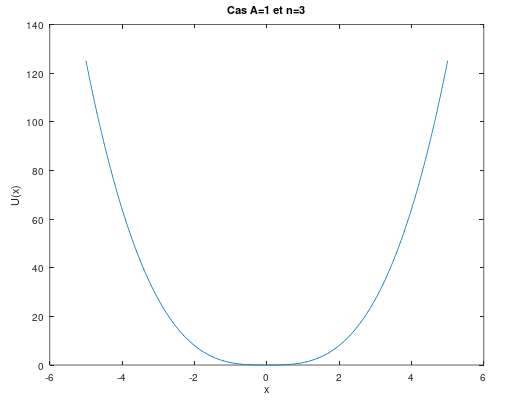
\includegraphics[width=10cm]{chapter_03_exercice_2a}
		\caption{$U = \lvert x \rvert^{n}$ pour $n \in \{1,2,3,4,5\}$}\label{FIG:3_2_a}
	\end{center}
\end{figure}

Dans ce cas pr\'ecis, commen\c{c}ons par d\'efinir les points d'arr\^et tels que $E=U$, soit $x = \pm\left(\dfrac{E}{A}\right)^{\frac{1}{n}}$. Cela permet d'\'ecrire l'\'equation (\ref{EQ:11_5}) telle que :
\bea
	\mathrm{T}(E) & = & \sqrt{2m}\int_{-\left(\frac{E}{A}\right)^{\frac{1}{n}}}^{+\left(\frac{E}{A}\right)^{\frac{1}{n}}}\dfrac{\mathrm{d}x}{\sqrt{E - A\lvert x \rvert^{n}}} \nonumber \\
	& = & 2\sqrt{2m}\int_{0}^{+\left(\frac{E}{A}\right)^{\frac{1}{n}}}\dfrac{\mathrm{d}x}{\sqrt{E - Ax^{n}}} \nonumber \\
	& = & 2\sqrt{\dfrac{2m}{E}}\int_{0}^{+\left(\frac{E}{A}\right)^{\frac{1}{n}}}\dfrac{\mathrm{d}x}{\sqrt{1 - \dfrac{Ax^{n}}{E}}}
\eea
car la fonction $U$ est paire, i.e. $U(x) = U(-x)$. En posant :
\be
	y = \left(\dfrac{A}{E}\right)^{\frac{1}{n}}x
\ee
qui permet d'\'ecrire :
\be
	\begin{cases}
		y^{n} = \dfrac{A}{E}x^{n} \\
		\mathrm{d}y = \left(\dfrac{A}{E}\right)^{\frac{1}{n}}\mathrm{d}x
	\end{cases}
\ee
et :
\be
	\begin{cases}
		x = 0 \Rightarrow y = 0 \\
		x = \left(\dfrac{E}{A}\right)^{\frac{1}{n}} \Rightarrow y = \left(\dfrac{A}{E}\right)^{\frac{1}{n}}\left(\dfrac{E}{A}\right)^{\frac{1}{n}} = 1
	\end{cases}
\ee
La p\'eriode $\mathrm{T}$ devient :
\bea
	\mathrm{T} & = & 2\sqrt{\dfrac{2m}{E}}\int_{0}^{1}\left(\dfrac{E}{A}\right)^{\frac{1}{n}}\dfrac{\mathrm{d}y}{\sqrt{1 - y^{n}}} \nonumber \\
	& = & 2\dfrac{\sqrt{2mE^{\frac{1}{n}-\frac{1}{2}}}}{A^{\frac{1}{n}}}\int_{0}^{1}\dfrac{\mathrm{d}y}{\sqrt{1 - y^{n}}}
\eea
De la m\^eme mani\`ere, en posant $u=y^{n}$, nous avons :
\be
	\begin{cases}
		y = 0 \Rightarrow u = 0 \\
		y = 1 \Rightarrow u = 1
	\end{cases}
\ee
ainsi que :
\be
	\begin{cases}
		y = u^{\frac{1}{n}} \Rightarrow y^{n-1} = u^{\frac{n-1}{n}} = u^{1 - \frac{1}{n}} \\
		ny^{n-1}\mathrm{d}y = \mathrm{d}u \Leftrightarrow \mathrm{d}y = \dfrac{u^{\frac{1}{n} - 1}}{n}\mathrm{d}u
	\end{cases}
\ee
Nous arrivons \`a :
\bea
	\mathrm{T} & = & 2\dfrac{\sqrt{2m}E^{\frac{1}{n}-\frac{1}{2}}}{A^{\frac{1}{n}}}\int_{0}^{1}\dfrac{u^{\frac{1}{n} - 1}\mathrm{d}u}{n(1-u)^{\frac{1}{2}}} \nonumber \\
	& = & 2\dfrac{\sqrt{2m}E^{\frac{1}{n}-\frac{1}{2}}}{nA^{\frac{1}{n}}}\int_{0}^{1}u^{\frac{1}{n} - 1}(1-u)^{\frac{-1}{2}}\mathrm{d}u \label{EQ:APP3_2_a}
\eea
Utilisons ici les int\'egrales d'Euler de premi\`ere esp\`ece, \emph{fonction Béta}, d\'efinies telles que :
\be
	\mathrm{B}(x,y) = \int_{0}^{1}\mathrm{t}^{x-1}(1-\mathrm{t})^{y-1}\mathrm{dt} = \dfrac{\Gamma(x)\Gamma(y)}{\Gamma(x+y)} \label{EQ:INT_EULER_BETA}
\ee
et celles de seconde esp\`ece, \emph{fonction Gamma} :
\be
	\Gamma(z) = \int_{0}^{+\infty}\mathrm{t}^{z-1}e^{-\mathrm{t}}\mathrm{dt} \label{EQ:INT_EULER_GAMMA}
\ee
L'\'equation (\ref{EQ:APP3_2_a}) s'\'ecrit alors :
\bea
	\mathrm{T} & = & 2\dfrac{\sqrt{2m}E^{\frac{1}{n}-\frac{1}{2}}}{nA^{\frac{1}{n}}}\mathrm{B}\left(\frac{1}{n},\frac{1}{2}\right) \nonumber \\
	& = & 2\dfrac{\sqrt{2m}E^{\frac{1}{n}-\frac{1}{2}}}{nA^{\frac{1}{n}}}\dfrac{\Gamma\left(\frac{1}{n}\right)\Gamma\left(\frac{1}{2}\right)}{\Gamma\left(\frac{1}{n}+\frac{1}{2}\right)} \nonumber
\eea
Or $\Gamma(1/2) = \sqrt{\pi}$, nous avons donc finalement :
\be
	\mathrm{T} = 2\dfrac{\sqrt{2\pi m}\Gamma\left(\frac{1}{n}\right)}{nA^{\frac{1}{n}}\Gamma\left(\frac{1}{n}+\frac{1}{2}\right)}E^{\frac{1}{n}-\frac{1}{2}}
\ee

\begin{figure}[htb!]
	\begin{center}
		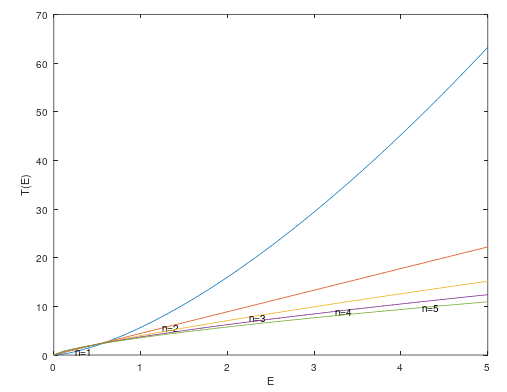
\includegraphics[width=10cm]{chapter_03_exercice_2a_result}
		\caption{$\mathrm{T}(E)$ pour $m=1$, $A=1$ et $n \in \{1,2,3,4,5\}$}\label{FIG:3_2_a_result}
	\end{center}
\end{figure}

\subsubsection{$U = -U_{0}/\cosh^{2}(\alpha x)$ avec $-U_{0} < E < 0$}

\begin{figure}[htb!]
	\begin{center}
		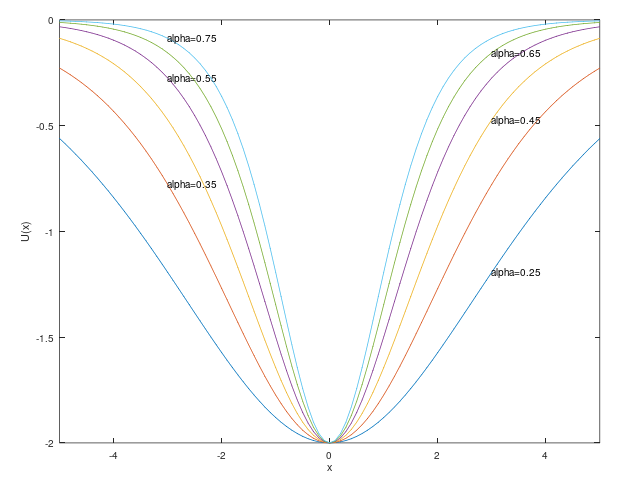
\includegraphics[width=10cm]{chapter_03_exercice_2b}
		\caption{$U = -2 / \cosh^{2}(\alpha x)$ pour $\alpha \in \{0.25,0.35,0.45,0.55,0.65,0.75\}$}\label{FIG:3_2_b}
	\end{center}
\end{figure}

Les point d'arr\^et sont toujours d\'efinis tels que $U=E$, i.e. :
\bea
	\cosh^{2}(\alpha x) & = & -\dfrac{U_{0}}{E} \nonumber \\
	\Leftrightarrow \alpha x & = & \pm \arccosh\left(\sqrt{\dfrac{-U_{0}}{E}}\right)
\eea
Ceci est possible car $-U_{0} < E < 0$ et donc $-U_{0}/E > 0$. Les points d'arr\^et sont donc :
\be
	x = \pm \dfrac{1}{\alpha}\arccosh\left(\sqrt{\dfrac{-U_{0}}{E}}\right)
\ee

L'\'equation (\ref{EQ:11_5}) peut donc s'\'ecrire :
\bea
	\mathrm{T}(E) & = & \sqrt{2m}\int_{-\frac{1}{\alpha}\arccosh\left(\sqrt{\frac{-U_{0}}{E}}\right)}^{\frac{1}{\alpha}\arccosh\left(\sqrt{\frac{-U_{0}}{E}}\right)}\dfrac{\mathrm{d}x}{\sqrt{E + \dfrac{U_{0}}{\cosh^{2}(\alpha x)}}} \nonumber \\
	& = & \sqrt{\dfrac{2m}{\lvert E \rvert}}\int_{-\frac{1}{\alpha}\arccosh\left(\sqrt{\frac{-U_{0}}{E}}\right)}^{\frac{1}{\alpha}\arccosh\left(\sqrt{\frac{-U_{0}}{E}}\right)}\dfrac{\mathrm{d}x}{\sqrt{1 + \dfrac{U_{0}}{E\cosh^{2}(\alpha x)}}}
\eea
car $E < 0$. En choisissant :
\be
	y = \sqrt{\frac{-U_{0}}{E}}\dfrac{1}{\cosh(\alpha x)}
\ee
nous obtenons pour les bornes de l'int\'egrale :
\be
	\begin{cases}
		x = -\frac{1}{\alpha}\arccosh\left(\sqrt{\frac{-U_{0}}{E}}\right) \Rightarrow y = -1 \\
		x = \frac{1}{\alpha}\arccosh\left(\sqrt{\frac{-U_{0}}{E}}\right) \Rightarrow y = 1 \\
	\end{cases}
\ee
et :
\bea
	y^{2} & = & \frac{-U_{0}}{E}\dfrac{1}{\cosh^{2}(\alpha x)} \nonumber \\
	\mathrm{d}y & = & \sqrt{\frac{-U_{0}}{E}}\dfrac{-\alpha}{\cosh^{2}(\alpha x)}\mathrm{d}x \nonumber \\
	\Leftrightarrow & = & -\alpha\sqrt{\frac{-U_{0}}{E}}\dfrac{E}{-U_{0}}y^{2}\mathrm{d}x \nonumber \\
	\Leftrightarrow \mathrm{d}x & = & -\sqrt{\frac{-U_{0}}{E}}\dfrac{\mathrm{d}y}{\alpha y^{2}}
\eea
La p\'eriode s'\'ecrit alors :
\bea
	\mathrm{T}(E) & = & \sqrt{\dfrac{2m}{\lvert E \rvert}}\int_{-1}^{1}\dfrac{y^{-2}\mathrm{d}y}{\sqrt{1-y^{2}}}\times \dfrac{-1}{\alpha}\sqrt{\dfrac{-U_{0}}{E}} \nonumber \\
	& = & -\dfrac{2}{\alpha}\sqrt{\dfrac{-U_{0}}{E}}\sqrt{\dfrac{2m}{\lvert E \rvert}}\int_{0}^{1}\dfrac{y^{-2}\mathrm{d}y}{\sqrt{1-y^{2}}}
\eea

En posant $u = y^{2}$, soit $y = u^{1/2}$ et $\mathrm{d}u = 2y\mathrm{d}y = 2u^{1/2}\mathrm{d}y \Leftrightarrow \mathrm{d}y = \frac{1}{2}u^{-1/2}\mathrm{d}u$, alors la p\'eriode devient :
\bea
	\mathrm{T}(E) & = & -\dfrac{2}{\alpha}\sqrt{\dfrac{-U_{0}}{E}}\sqrt{\dfrac{2m}{\lvert E \rvert}}\int_{0}^{1}\frac{1}{2}\dfrac{u^{-3/2}\mathrm{d}u}{(1-u)^{1/2}} \nonumber \\
	& = & -\dfrac{1}{\alpha}\sqrt{\dfrac{-U_{0}}{E}}\sqrt{\dfrac{2m}{\lvert E \rvert}} \mathrm{B}\left(-\frac{1}{2},\frac{1}{2}\right) \nonumber \\
	& = & \dfrac{2\pi}{\alpha}\sqrt{\dfrac{-U_{0}}{E}}\sqrt{\dfrac{2m}{\lvert E \rvert}}
\eea
car $\Gamma(0) = 1$, $\Gamma(\frac{1}{2}) = \sqrt{\pi}$ et $\Gamma(-\frac{1}{2}) = -2\sqrt{\pi}$. Ici, je trouve une solution diff\'erente de celle propos\'ee par le livre qui est : $\mathrm{T}(E) = \dfrac{\pi}{\alpha}\sqrt{\dfrac{2m}{\lvert E \rvert}}$ et j'avoue ne pas savoir en quoi la p\'riode ne pourrait pas d\'ependre de la profondeur du puits d'\'energie potentielle $U_{0}$.

\subsubsection{$U = U_{0}\tan^{2}(\alpha x)$}

\begin{figure}[htb!]
	\begin{center}
		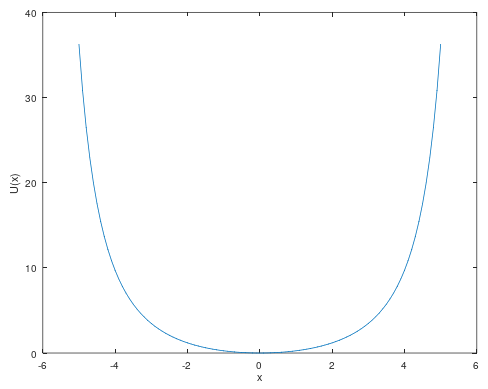
\includegraphics[width=10cm]{chapter_03_exercice_2c}
		\caption{$U = 4\tan^{2}(\alpha x)$ pour $\alpha \in \{0.25,0.35,0.45,0.55,0.65,0.75\}$}\label{FIG:3_2_c}
	\end{center}
\end{figure}
\chapter{Probl\`emes de chocs des particules}

\section{D\'esint\'egrations de deux particules}

\subsection{Relation entre $\theta_{1}$ et $\theta_{2}$ dans <<~l~>>}

L'objectif ici est d'obtenir la relation entre $\theta_{1}$ et $\theta_{2}$ dans le r\'ef\'erentiel <<~l~>> dans le cadre de la d\'esint\'egration d'une particule de vitesse initiale $\vec{V}$ en deux particules r\'esultantes de masse respective $m_{1}$ et $m_{2}$. Dans le r\'ef\'erentiel <<~c~>>, le centre d'inertie est immobile, aussi :
\be
	\vec{R} = \dfrac{m_{1}\vec{r}_{10} + m_{2}\vec{r}_{20}}{m_{1} + m_{2}}
\ee
donne :
\bea
	\dfrac{\mathrm{d}\vec{R}}{\mathrm{dt}} & = & \vec{0} \nonumber \\
	m_{1}\vec{v}_{10} + m_{2}\vec{v}_{20} & = & \vec{0}
\eea
qui permet d'\'ecrire :
\bea
	m_{1}\lVert \vec{v}_{10} \rVert & = & m_{2}\lVert \vec{v}_{20} \rVert \nonumber \\
	\dfrac{m_{1}}{m_{2}} & = & \dfrac{v_{20}}{v_{10}}
\eea
mais \'egalement en utilisant le r\'esultat pr\'ec\'edent :
\bea
	m_{1}^{2}v_{10}^{2} + m_{2}^{2}v_{20}^{2} + 2 m_{1}m_{2}v_{10}v_{20}\cos(\theta_{10} + \theta_{20}) & = & 0 \nonumber \\
	m_{1}^{2}v_{10}^{2} + m_{1}^{2}v_{10}^{2} + 2 m_{1}^{2}v_{10}^{2}\cos(\theta_{10} + \theta_{20}) & = & 0 \nonumber \\
	\cos(\theta_{10} + \theta_{20}) & = & -1 \nonumber \\
	\theta_{10} + \theta_{20} & = & \pi
\eea

Les particules r\'esultantes n'interagissant pas l'une sur l'autre, la relation (\ref{EQ:16_5}) est applicable \`a l'une et l'autre telle que :
\bea
	\tan\theta_{1} = \dfrac{v_{10}\sin\theta_{10}}{V + v_{10}\cos\theta_{10}} & \text{ et } & \tan\theta_{2} = \dfrac{v_{20}\sin\theta_{20}}{V + v_{20}\cos\theta_{20}} \nonumber \\
	v_{10}\cos\theta_{10} + V = \dfrac{v_{10}\sin\theta_{10}}{\tan\theta_{1}} & \text{ et } & v_{20}\cos\theta_{20} + V = \dfrac{v_{20}\sin\theta_{20}}{\tan\theta_{2}} \nonumber \\
	V + v_{10}\cos\theta_{10} = \dfrac{v_{10}\sin\theta_{10}}{\tan\theta_{1}} & \text{ et } & V - v_{20}\cos\theta_{10} = \dfrac{v_{20}\sin\theta_{10}}{\tan\theta_{2}}
\eea
La premi\`ere relation permet d'\'ecrire :
\be
	\cos\theta_{10} = \dfrac{\sin\theta_{10}}{\tan\theta_{1}} - \dfrac{V}{v_{10}}
\ee
qui, inject\'ee dans la seconde :
\bea
	V - \dfrac{v_{20}\sin\theta_{10}}{\tan\theta_{1}} + \dfrac{v_{20}V}{v_{10}} & = & \dfrac{v_{20}\sin\theta_{10}}{\tan\theta_{2}} \nonumber \\
	\left(1 + \dfrac{v_{20}}{v_{10}}\right)V & = & \left(\dfrac{1}{\tan\theta_{1}} + \dfrac{1}{\tan\theta_{2}}\right)v_{20}\sin\theta_{10} \nonumber \\
	\sin\theta_{10} & = & V\dfrac{\frac{1}{v_{10}} + \frac{1}{v_{20}}}{\left(\frac{1}{\tan\theta_{1}} + \frac{1}{\tan\theta_{2}}\right)}
\eea
et par voie de cons\'equence :
\be
	\cos\theta_{10} = V\dfrac{\frac{1}{v_{10}} + \frac{1}{v_{20}}}{\left(1 + \frac{\tan\theta_{1}}{\tan\theta_{2}}\right)} - \dfrac{V}{v_{10}}
\ee
En utilisant la relation bien connue : $\cos^{2} + \sin^{2} = 1$, nous pouvons continuer avec $\theta_{10}$ telle que :
\be
	V^{2}\dfrac{\left(\frac{1}{v_{10}} + \frac{1}{v_{20}}\right)^{2}}{\left(\frac{1}{\tan\theta_{1}} + \frac{1}{\tan\theta_{2}}\right)^{2}} + V^{2}\dfrac{\left(\frac{1}{v_{10}} + \frac{1}{v_{20}}\right)^{2}}{\left(1 + \frac{\tan\theta_{1}}{\tan\theta_{2}}\right)^{2}} + \dfrac{V^{2}}{v_{10}^{2}} - 2\dfrac{V^{2}}{v_{10}}\dfrac{\frac{1}{v_{10}} + \frac{1}{v_{20}}}{\left(\frac{1}{\tan\theta_{1}} + \frac{1}{\tan\theta_{2}}\right)} = 1
\ee
Sachant que :
\be
	\dfrac{1}{v_{10}} + \dfrac{1}{v_{20}} = \frac{1}{v_{10}}\left( 1 + \frac{v_{10}}{v_{20}}\right) =  \frac{1}{v_{10}}\left( 1 + \frac{m_{2}}{m_{1}}\right)
\ee
l'\'equation devient :
\bea
	\dfrac{V^{2}}{v_{10}^{2}}\dfrac{\left(1 + \frac{m_{2}}{m_{1}}\right)^{2}}{\left(\frac{1}{\tan\theta_{1}} + \frac{1}{\tan\theta_{2}}\right)^{2}} + \dfrac{V^{2}}{v_{10}^{2}}\dfrac{\left(1 + \frac{m_{2}}{m_{1}}\right)^{2}}{\left(1 + \frac{\tan\theta_{1}}{\tan\theta_{2}}\right)^{2}} + \dfrac{V^{2}}{v_{10}^{2}} - 2\dfrac{V^{2}}{v_{10}^{2}}\dfrac{1 + \frac{m_{2}}{m_{1}}}{\left(\frac{1}{\tan\theta_{1}} + \frac{1}{\tan\theta_{2}}\right)} & = & 1 \nonumber \\
	\dfrac{(m_{1} + m_{2})^{2}}{m_{1}^{2}\left(\frac{1}{\tan\theta_{1}} + \frac{1}{\tan\theta_{2}}\right)^{2}} + \dfrac{(m_{1} + m_{2})^{2}}{m_{1}^{2}\left(1 + \frac{\tan\theta_{1}}{\tan\theta_{2}}\right)^{2}} - 2\dfrac{(m_{1} + m_{2})}{m_{1}\left(\frac{1}{\tan\theta_{1}} + \frac{1}{\tan\theta_{2}}\right)} & = & \dfrac{v_{10}^{2}}{V^{2}} - 1 \nonumber \\
	\dfrac{m_{1} + m_{2}}{m_{1}\left(\frac{1}{\tan\theta_{1}} + \frac{1}{\tan\theta_{2}}\right)^{2}} + \dfrac{m_{1} + m_{2}}{m_{1}\left(1 + \frac{\tan\theta_{1}}{\tan\theta_{2}}\right)^{2}} - \dfrac{2}{\left(\frac{1}{\tan\theta_{1}} + \frac{1}{\tan\theta_{2}}\right)} & = & \dfrac{(v_{10}^{2} - V^{2})m_{1}}{(m_{1} + m_{2})V^{2}} \nonumber \\
\eea
Or il convient de d\'evelopper :
\be
	\dfrac{1}{\tan\theta_{1}} + \dfrac{1}{\tan\theta_{2}} = \dfrac{\cos\theta_{1}}{\sin\theta_{1}} + \dfrac{\cos\theta_{2}}{\sin\theta_{2}} = \dfrac{\cos\theta_{1}\sin\theta_{2} + \sin\theta_{1}\cos\theta_{2}}{\sin\theta_{1}\sin\theta_{2}} = \dfrac{\sin(\theta_{1} + \theta_{2})}{\sin\theta_{1}\sin\theta_{2}}
\ee
et
\bea
	1 + \dfrac{\tan\theta_{1}}{\tan\theta_{2}} & = & \dfrac{\tan\theta_{1} + \tan\theta_{2}}{\tan\theta_{2}} = \left(\dfrac{\cos\theta_{1}}{\sin\theta_{1}} + \dfrac{\cos\theta_{2}}{\sin\theta_{2}}\right)\dfrac{\cos\theta_{2}}{\sin\theta_{2}} \nonumber \\
	& = & \dfrac{(\cos\theta_{1}\sin\theta_{2} + \sin\theta_{1}\cos\theta_{2})\cos\theta_{2}}{\cos\theta_{1}\cos\theta_{2}\sin\theta_{2}} = \dfrac{\sin(\theta_{1} + \theta_{2})}{\cos\theta_{1}\sin\theta_{2}}
\eea
L'\'equation principale devient alors :
\be
	\dfrac{(v_{10}^{2} - V^{2})m_{1}}{(m_{1} + m_{2})V^{2}}\sin^{2}(\theta_{1} + \theta_{2}) = \dfrac{m_{1} + m_{2}}{m_{1}}\sin^{2}\theta_{2} - 2\cos\theta_{1}\sin\theta_{2}\sin(\theta_{1} + \theta_{2})
\ee
Toutefois :
\bea
	\cos\theta_{1}\sin\theta_{2}\sin(\theta_{1} + \theta_{2}) & = & \cos\theta_{1}\sin\theta_{2}(\cos\theta_{1}\sin\theta_{2} + \sin\theta_{1}\cos\theta_{2}) \nonumber \\
	& = & \cos^{2}\theta_{1}\sin^{2}\theta_{2} + \cos\theta_{1}\sin\theta_{1}\cos\theta_{2}\sin\theta_{2} \nonumber \\
	& = & \sin^{2}\theta_{2} - \sin^{2}\theta_{1}\sin^{2}\theta_{2} + \cos\theta_{1}\sin\theta_{1}\cos\theta_{2}\sin\theta_{2} \nonumber \\
	& = & \sin^{2}\theta_{2} - \sin\theta_{1}\sin\theta_{2}(\sin\theta_{1}\sin\theta_{2} - \cos\theta_{1}\cos\theta_{2}) \nonumber \\
	& = & \sin^{2}\theta_{2} + \sin\theta_{1}\sin\theta_{2}\cos(\theta_{1} + \theta_{2})
\eea
ce qui permet d'avancer ainsi :
\bea
	\dfrac{(v_{10}^{2} - V^{2})m_{1}}{(m_{1} + m_{2})V^{2}}\sin^{2}(\theta_{1} + \theta_{2}) & = & \dfrac{m_{1} + m_{2}}{m_{1}}\sin^{2}\theta_{2} - 2\sin^{2}\theta_{2} - 2\sin\theta_{1}\sin\theta_{2}\cos(\theta_{1} + \theta_{2})\nonumber \\
	& = & \dfrac{m_{2}}{m_{1}}\sin^{2}\theta_{2} + \sin^{2}\theta_{2} - 2\sin^{2}\theta_{2} - 2\sin\theta_{1}\sin\theta_{2}\cos(\theta_{1} + \theta_{2})\nonumber \\
	& = & \dfrac{m_{2}}{m_{1}}\sin^{2}\theta_{2} - \sin^{2}\theta_{2} - 2\sin\theta_{1}\sin\theta_{2}\cos(\theta_{1} + \theta_{2})
\eea

\subsection{Distribution des directions dans <<~l~>>}

Pour \'etablie la distribution des directions des particules r\'esultantes dans le r\'ef\'erentiel <<~l~>>, nous allons repartir de l'\'equation (\ref{EQ:16_6}) qui apporte la solution pour deux domaines diff\'erents.

\subsubsection{$v_{0} > V$}

Dans ce cas, $\theta \in [0;\pi]$ \`a la vue de la figure (\ref{FIG:4_14}) et l'\'equation (\ref{EQ:16_6}) s'\'ecrit :
\be
	\cos\theta_{0} = -\dfrac{V}{v_{0}}\sin^{2}\theta + \cos\theta\sqrt{1 - \dfrac{V^{2}}{v_{0}^{2}}\sin^{2}\theta}
\ee
La distribution $\dfrac{\mathrm{d}\omega_{0}}{4\pi}$ vaut $\dfrac{1}{2}\sin\theta_{0}\mathrm{d}\theta_{0} = -\dfrac{\mathrm{d}(\cos\theta_{0})}{2}$ selon l'\'equation (\ref{EQ:16_7}). Cela permet donc d'\'ecrire avec la relation pr\'ec\'edente :
\bea
	\begin{Bmatrix}\dfrac{\mathrm{d}\omega_{0}}{4\pi}\end{Bmatrix}_{1} & = & \dfrac{V}{v_{0}}\sin\theta\cos\theta\mathrm{d}\theta + \dfrac{\sin\theta}{2}\sqrt{1 - \dfrac{V^{2}}{v_{0}^{2}}\sin^{2}\theta}\mathrm{d}\theta - \dfrac{\cos\theta}{4}\dfrac{-2\dfrac{V^{2}}{v_{0}^{2}}\sin\theta\cos\theta\mathrm{d}\theta}{\sqrt{1 - \dfrac{V^{2}}{v_{0}^{2}}\sin^{2}\theta}} \nonumber \\
	& = & \dfrac{V}{v_{0}}\sin\theta\cos\theta\mathrm{d}\theta + \dfrac{\mathrm{d}\theta}{2\sqrt{1 - \dfrac{V^{2}}{v_{0}^{2}}\sin^{2}\theta}}\left(\sin\theta - \dfrac{V^{2}}{v_{0}^{2}}\sin^{3}\theta + \dfrac{V^{2}}{v_{0}^{2}}\sin\theta\cos^{2}\theta\right) \nonumber \\
	& = & \dfrac{1}{2}\sin\theta\mathrm{d}\theta\left[2\dfrac{V}{v_{0}}\cos\theta + \dfrac{V^{2}}{v_{0}^{2}\sqrt{1 - \dfrac{V^{2}}{v_{0}^{2}}\sin^{2}\theta}}(\dfrac{v_{0}^{2}}{V^{2}} + \cos^{2}\theta - \sin^{2}\theta)\right] \nonumber \\
	& = & \dfrac{1}{2}\sin\theta\left[2\dfrac{V}{v_{0}}\cos\theta + \dfrac{1+\dfrac{V^{2}}{v_{0}^{2}}\cos(2\theta)}{\sqrt{1 - \dfrac{V^{2}}{v_{0}^{2}}\sin^{2}\theta}}\right]\mathrm{d}\theta\label{EQ:16_EX2A}
\eea

\begin{figure}[htb!]
	\begin{center}
		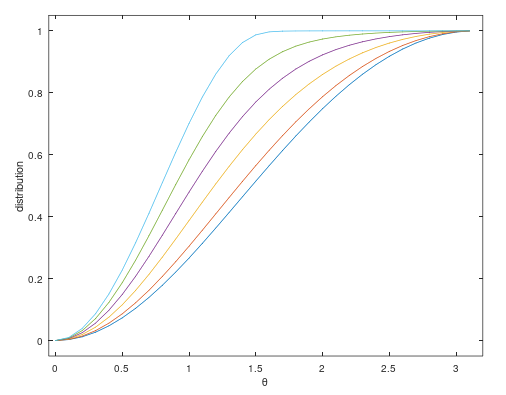
\includegraphics[width=10cm]{chapter_04_paragraph_16_exercice_2a}
		\caption{Exemples de distribution pour diff\'erentes valeurs de $\frac{V}{v_{0}}$, de 0.1 à 0.99, par int\'egration de l'\'equation (\ref{EQ:16_EX2A})}\label{FIG:4_16_EX2A}
	\end{center}
\end{figure}

\subsubsection{$v_{0} < V$}

Dans ce cas, la m\^eme s\'equence calculatoire am\`ene \`a \'ecrire pour $\theta \in [0;\theta_{max}]$ :
\be
	\begin{Bmatrix}\dfrac{\mathrm{d}\omega_{0}}{4\pi}\end{Bmatrix}_{2} = \dfrac{1}{2}\sin\theta\left[2\dfrac{V}{v_{0}}\cos\theta - \dfrac{1 + \dfrac{V^{2}}{v_{0}^{2}}\cos(2\theta)}{\sqrt{1 - \dfrac{V^{2}}{v_{0}^{2}}\sin^{2}\theta}}\right]\mathrm{d}\theta
\ee
sachant qu'il faut prendre cette fois-ci dans l'\'equation (\ref{EQ:16_6}) les deux solutions, celles avec le signe - et celle avec le signe +, d\'eduite pr\'ec\`edemment. Ainsi la distribution totale pour $v_{0} < V$ s'obtient en faisant :
\be
	\begin{Bmatrix}\dfrac{\mathrm{d}\omega_{0}}{4\pi}\end{Bmatrix}_{1} - \begin{Bmatrix}\dfrac{\mathrm{d}\omega_{0}}{4\pi}\end{Bmatrix}_{2} = \dfrac{1 + \dfrac{V^{2}}{v_{0}^{2}}\cos(2\theta)}{\sqrt{1 - \dfrac{V^{2}}{v_{0}^{2}}\sin^{2}\theta}}\sin\theta\mathrm{d}\theta\label{EQ:16_EX2B}
\ee

\begin{figure}[htb!]
	\begin{center}
		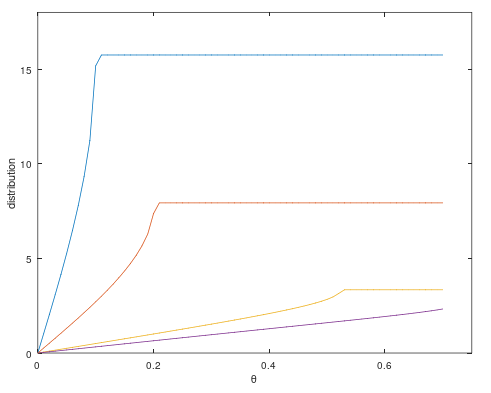
\includegraphics[width=10cm]{chapter_04_paragraph_16_exercice_2b}
		\caption{Exemples de distribution pour diff\'erentes valeurs de $\frac{V}{v_{0}}$, de 1.5 à 10, par int\'egration de l'\'equation (\ref{EQ:16_EX2B})}\label{FIG:4_16_EX2B}
	\end{center}
\end{figure}

\subsection{Intervalles angulaires dans <<~l~>>}

Dans le r\'ef\'erentiel <<~l~>>, d\'eterminons l'angle $\theta$ d\'efini comme la somme $\theta_{1} + \theta_{2}$ :
\bea
	\tan\theta & = & \tan(\theta_{1} + \theta_{2}) = \dfrac{\tan\theta_{1} + \tan\theta_{2}}{1 - \tan\theta_{1}\tan\theta_{2}} \nonumber \\
	& = & \dfrac{\dfrac{v_{10}\sin\theta_{10}}{V + v_{10}\cos\theta_{10}} + \dfrac{v_{20}\sin\theta_{20}}{V + v_{20}\cos\theta_{20}}}{1 - \dfrac{v_{10}\sin\theta_{10}}{V + v_{10}\cos\theta_{10}}\dfrac{v_{20}\sin\theta_{20}}{V + v_{20}\cos\theta_{20}}} \nonumber \\
\eea
or $\theta_{20} = \pi - \theta_{10}$, donc :
\bea
	\tan\theta & = & \dfrac{\dfrac{v_{10}\sin\theta_{10}}{V + v_{10}\cos\theta_{10}} + \dfrac{v_{20}\sin\theta_{10}}{V - v_{20}\cos\theta_{10}}}{1 - \dfrac{v_{10}\sin\theta_{10}}{V + v_{10}\cos\theta_{10}}\dfrac{v_{20}\sin\theta_{10}}{V - v_{20}\cos\theta_{10}}} \nonumber \\
	& = & \dfrac{v_{10}\sin\theta_{10}(V - v_{20}\cos\theta_{10}) + v_{20}\sin\theta_{10}(v_{10}\cos\theta_{10} + V)}{(V + v_{10}\cos\theta_{10})(V - v_{20}\cos\theta_{10}) - v_{10}v_{20}\sin^{2}\theta_{10}} \nonumber \\
	& = & \dfrac{v_{10}V\sin\theta_{10} - v_{10}v_{20}\cos\theta_{10}\sin\theta_{10} + v_{10}v_{20}\cos\theta_{10}\sin\theta_{10} + v_{20}V\sin\theta_{10}}{v_{10}V\cos\theta_{10} - v_{10}v_{20}\cos^{2}\theta_{10} + V^{2} - v_{20}V\cos\theta_{10} - v_{10}v_{20}\sin^{2}\theta_{10}} \nonumber \\
	& = & \dfrac{(v_{10} + v_{20})V\sin\theta_{10}}{V^{2} - v_{10}v_{20} + (v_{10} - v_{20})V\cos\theta_{10}}
\eea

\section{Chocs \'elastiques de deux particules}

Dans le r\'ef\'erentiel <<~l~>>, exprimons les vitesses apr\`es le choc $v'_{1}$ et $v'_{2}$ en fonction de l'angle de d\'eviation sous lequel elles s'\'ecartent, sachant qu'avant le choc $v_{2} = 0$ et donc $v_{1} = v$.

Puisque la grandeur $2OB$ est un diam\`etre du cercle de rayon $mv$, nous avons $p'_{2} = 2OB\cos\theta_{2}$, donc :
\be
	v'_{2} = \dfrac{2OB}{m_{2}}\cos\theta_{2} = \dfrac{2mv}{m_{2}}\cos\theta_{2}
\ee
avec $m$ la masse r\'eduite du syst\`eme compos\'e des deux particules.

Ensuite, nous utilisons la formule d'Al-Kashi dans le triangle form\'e des points $A$, $O$ et $C$, voir la figure (\ref{FIG:4_16}) pour faire intervenir l'angle $\theta_{1}$ tel que :
\bea
	OC^{2} & = & AO^{2} + {p'}_{1}^{2} - 2 AOp'_{1}\cos\theta_{1} \nonumber \\
	m^{2}v^{2} & = & \dfrac{m_{1}^{2}}{m_{2}^{2}}OB^{2} + m_{1}^{2}{v'}_{1}^{2} - 2\dfrac{m_{1}^{2}}{m_{2}}OBv'_{1}\cos\theta_{1} \nonumber \\
	\left(1 - \dfrac{m_{1}^{2}}{m_{2}^{2}}\right)m^{2}v^{2} & = & m_{1}^{2}{v'}_{1}^{2} - 2\dfrac{m_{1}^{2}}{m_{2}}mvv'_{1}\cos\theta_{1} \nonumber \\
	\dfrac{(m_{2} + m_{1})(m_{2} - m_{1})}{m_{2}^{2}}m^{2} & = & m_{1}^{2}\dfrac{v'_{1}}{v}^{2} - 2\dfrac{m_{1}^{2}}{m_{2}}m\dfrac{v'_{1}}{v}\cos\theta_{1} \nonumber \\
	\dfrac{(m_{2} + m_{1})(m_{2} - m_{1})m_{1}^{2}m_{2}^{2}}{m_{2}^{2}(m_{1} + m_{2})} & = & m_{1}^{2}\dfrac{v'_{1}}{v}^{2} - 2\dfrac{m_{1}^{2}}{m_{2}}m\dfrac{v'_{1}}{v}\cos\theta_{1} \nonumber \\
	0 & = & \left(\dfrac{v'_{1}}{v}\right)^{2} - 2\dfrac{m}{m_{2}}\dfrac{v'_{1}}{v}\cos\theta_{1} + \dfrac{m_{1} - m_{2}}{m_{1} + m_{2}}
\eea

Il s'agit d'une \'equation du second degr\'e en $v'_{1}/v$ dont les solutions sont :
\bea
	\dfrac{v'_{1}}{v} & = & \dfrac{1}{2}\left(\dfrac{2m_{1}m_{2}}{m_{2}(m_{1} + m_{2})}\cos\theta_{1} \pm \sqrt{\dfrac{4m_{1}^{2}m_{2}^{2}}{m_{2}^{2}(m_{1} + m_{2})^{2}}\cos^{2}\theta_{1} - \dfrac{4(m_{1} - m_{2})}{m_{2}(m_{1} + m_{2})}}\right) \nonumber \\
	& = & \dfrac{m_{1}}{m_{1} + m_{2}}\cos\theta_{1} \pm \sqrt{\dfrac{m_{1}^{2}}{(m_{1} + m_{2})^{2}}\cos^{2}\theta_{1} - \dfrac{m_{1}^{2} - m_{2}^{2}}{(m_{1} + m_{2})^{2}}} \nonumber \\
	& = & \dfrac{m_{1}}{m_{1} + m_{2}}\cos\theta_{1} \pm \dfrac{1}{m_{1} + m_{2}}\sqrt{m_{2}^{2} + (\cos^{2}\theta_{1} - 1)m_{1}^{2}} \nonumber \\
	& = & \dfrac{m_{1}}{m_{1} + m_{2}}\cos\theta_{1} \pm \dfrac{m_{2}}{m_{1} + m_{2}}\sqrt{1 + \dfrac{m_{1}^{2}}{m_{2}^{2}}\sin^{2}\theta_{1}}
\eea
De mani\`ere \'equivalente \`a l'\'equation (\ref{EQ:16_6}), pour $m_{1} > m_{2}$, la solution est univoque avec le signe $+$ alors que pour $m_{1} < m_{2}$, les deux solutions sont admises. La repr\'esentation de ces solutions est \'egalement similaire \`a ce qui est repr\'esent\'e sur les figures (\ref{FIG:4_14A}) et (\ref{FIG:4_14B}).

\section{Diffusion des particules}

\subsection{Diffusion par une bille solide}

\subsection{\'Energie perdue}

\subsection{Cas d'un champ $\propto r^{-n}$}

\subsection{Cas d'un champ $U = -\alpha / r^{2}$}

\subsection{Cas d'un champ $U = -\alpha / r^{n}$}

\subsection{Cas d'un champ suivant la loi de Newton}

\subsection{M\'ethode d'inversion de Firsov}

Oleg Firsov, 1953 cit\'e dans un article de 1971\footnote{Uniqueness of the Firsov Inversion Method and Focusing Potentials, Yu.N. Demkov, V.N. Ostrovskii, et N.B. Berezina}
\chapter{Petites oscillations}

\section{Oscillations lin\'eaires libres}

\subsection{Amplitude et phase initiale}

En ayant $x(t=0) = x_{0}$ et $v(t=0) = v_{0}$ et en prenant la formule (\ref{EQ:21_8}), cela permet d'\'ecrire :
\benn
	\begin{cases}
		x_{0} = a\cos\alpha \\
		v_{0} = -a\omega\sin\alpha
	\end{cases}
\eenn
donc :
\benn
	\begin{cases}
		\tan\alpha = \dfrac{-v_{0}}{\omega x_{0}} \\
		\\
		v_{0}^{2} + \omega^{2}x_{0}^{2} = a^{2}\omega^{2}\text{ donc } a =  \sqrt{x_{0}^{2} + \dfrac{v_{0}^{2}}{\omega^{2}}}
	\end{cases}
\eenn

\subsection{Mol\'ecules diatomiques}

L'isotope d'un atome est ce m\^eme atome mais avec un nombre de neutrons diff\'erents. En cons\'equence, l'\'energie potentielle d'interactions n'est pas modifi\'ee. La formule (\ref{EQ:21_5}) appliqu\'ee aux deux composantes de la mol\'ecule diatomique devient :
\benn
	\begin{cases}
		\ddot{x}_{1} + \frac{k}{m_{1}}x_{1}^{2} = 0 \\
		\ddot{x}_{2} + \frac{k}{m_{2}}x_{2}^{2} = 0 \\
	\end{cases}
\eenn
En d\'efinissant $X = x_{1} + x_{2}$, nous avons :
\benn
	\ddot{X} + k\left(\dfrac{1}{m_{1}} + \dfrac{1}{m_{2}}\right)X^{2} = 0
\eenn
Et en appliquant le m\^eme raisonnement \`a la seconde mol\'ecule, nous avons :
\benn
	\ddot{X'} + k\left(\dfrac{1}{m_{1}} + \dfrac{1}{m_{2}}\right){X'}^{2} = 0
\eenn
ce qui permet finalement d'\'ecrire le rapport des fr\'equences entre les deux mol\'ecules diatomiques :
\benn
	\dfrac{\omega'}{\omega} = \sqrt{\dfrac{k'}{k}\dfrac{m_{1}m_{2}(m'_{1} + m'_{2})}{m'_{1}m'_{2}(m_{1} + m_{2})}}
\eenn
et comme il s'agit d'isotopes et que l'int\'eraction est donc la m\^eme alors $k = k'$.

\subsection{Fr\'equence d'oscillations pour un point sur une droite}

\begin{figure}[htb!]
	\begin{center}
		\begin{picture}(100,150)(0,0)
			%axis
			\linethickness{0.05mm}
			\multiput(0,0)(10,0){10}{\line(1,0){8}}\put(102,-2){$x$}
			\multiput(50,0)(0,10){10}{\line(0,1){8}}\put(55,47){$l$}
			%mass
			\put(40,100){\line(1,0){20}}\put(47,102){$A$}
			\put(25,0){\color{black}\circle*{10}}\put(20,-12){$m$}
			%spring
			\linethickness{0.05mm}
			\multiput(25,0)(3,12){8}{\line(1,4){2}}
			\multiput(27,10)(3,12){8}{\color{black}\circle*{1}}
		\end{picture}
		\caption{Oscillations contraintes par le d\'eplacement sur une droite}\label{FIG:21_EX3_1}
	\end{center}
\end{figure}

Quand le ressort est de longueur $l$, soit $x = 0$, alors il est tendu avec une force $F$. Puisque nous sommes dans l'hypoth\`ese de petites oscillations, soit de petits d\'eplacements de la masse $x$, alors la relation (\ref{EQ:5_8}) s'applique et permet d'\'ecrire : $U = F\delta l$ avec $\delta l$ l'allongement du ressort. En appliquant Pythagore :
\benn
	(l + \delta l)^{2} = l^{2} + x^{2} \Leftrightarrow l^{2} + \delta l^{2} + 2l\delta l = l^{2} + x^{2} \Rightarrow \delta l = \dfrac{x^{2}}{2l}
\eenn
en n\'egligeant $\delta l^{2}$ en premi\`ere approximation. L'\'energie totale de la masse $m$ vaut :
\benn
	E = T + U = \dfrac{m}{2}\dot{x}^{2} + \dfrac{F}{2l}x^{2} = \dfrac{m}{2}\left(\dot{x}^{2} + \dfrac{F}{ml}x^{2}\right)
\eenn
ce qui permet d'en conclure directement :
\benn
	\omega^{2} = \dfrac{F}{ml}
\eenn

\subsection{Fr\'equence d'oscillations pour un point sur un cercle}

\begin{figure}[htb!]
	\begin{center}
		\begin{picture}(100,150)(0,0)
			%lengths
			\linethickness{0.05mm}
			\put(50,90){\vector(0,-1){35}}
			\put(49,92){$l$}
			\put(50,102){\vector(0,1){48}}
			\put(50,23){\vector(0,-1){23}}
			\put(49,25){$r$}
			\put(50,33){\vector(0,1){22}}
			%circle
			\put(50,0){\line(-1,2){25}}
			\qbezier(50,55)(-5,50)(-5,0)
			\qbezier(50,55)(105,55)(105,0)
			%angle
			\qbezier(50,10)(47,10)(45,8)
			\put(43,15){$\varphi$}
			%mass
			\put(40,150){\line(1,0){20}}\put(47,152){$A$}
			\put(25,50){\color{black}\circle*{10}}\put(18,38){$m$}
			%spring
			\linethickness{0.05mm}
			\multiput(25,50)(3,12){8}{\line(1,4){2}}
			\multiput(27,60)(3,12){8}{\color{black}\circle*{1}}
		\end{picture}
		\caption{Oscillations contraintes par le d\'eplacement sur une portion de cercle}\label{FIG:21_EX3_2}
	\end{center}
\end{figure}

Nous utilisons les m\^emes hypoth\`eses et la m\^eme m\'ethode que pour l'exercice pr\'ec\'edent, \`a l'exception du fait que la situation g\'eom\'etrique oblige \`a utiliser la g\'en\'eralisation du th\'eor\`eme de Pythagore, \`a savoir la formule d'Al-Kashi :
\bea
	(l + \delta l)^{2} & = & (r + l)^{2} + r^{2} - 2(r + l)r\cos\varphi \nonumber \\
	l^{2} + \delta l^{2} + 2l\delta l & = & r^{2} + l^{2} + 2rl + r^{2} - 2(r + l)r\cos\varphi \Leftrightarrow 2l\delta l = 2r^{2} + 2lr - 2(r + l)r\cos\varphi \nonumber \\
	\delta l & = & \dfrac{r(r + l)(1 - \cos\varphi)}{l} = \dfrac{r(r + l)}{2l}\varphi^{2} \nonumber
\eea
en utilisant l'hypoth\`ese de petits d\'eplacements qui permet de n\'egliger la quantité $\delta l^{2}$ et d'utiliser le d\'eveloppement en s\'erie de Taylor au premier ordre pour $(1 - \cos\varphi)$ tel que :
\benn
	\cos\varphi = \cos(0) - \sin(0)\varphi - \dfrac{1}{2}\cos(0)\varphi^{2} \Leftrightarrow \cos\varphi = 1 - \dfrac{1}{2}\varphi^{2}
\eenn
L'\'energie totale s'\'ecrit :
\bea
	E & = & T + U = \dfrac{mr{2}\dot{\varphi}^{2}}{2} + \dfrac{r(r + l)F}{2l}\varphi^{2} \nonumber \\
	& = & \dfrac{m}{2}\left(r^{2}\dot{\varphi}^{2} + \dfrac{r(r + l)F}{ml}\varphi^{2}\right) = \dfrac{m}{2}\left((r\dot{\varphi})^{2} + \dfrac{(r + l)F}{mlr}(r\varphi)^{2}\right) \nonumber
\eea
donc, la fr\'equence d'oscillations s'\'ecrit :
\benn
	\omega^{2} = \dfrac{(r + l)F}{mlr}
\eenn

\subsection{Oscillations du pendule plan}

Pour d\'eterminer la fr\'equence des oscillations, nous reprendrons la formule (\ref{EQ:13_EX3_1}) pr\'ealablement \'etablie dans ce contexte, voir la figure (\ref{FIG:1_2}). L'\'energie totale s\'ecrit alors dans sa forme g\'en\'erale :
\benn
	E = \dfrac{m_{2}l^{2}\dot{\varphi}^{2}}{2}\left(1 - \dfrac{m_{2}\cos^{2}\varphi}{(m_{1} + m_{2})}\right) - m_{2}gl\cos\varphi
\eenn
qui peut se d\'evelopper en utilisant l'approximation au second ordre $\cos\varphi = 1 - \dfrac{1}{2}\varphi^{2}$ :
\benn
	E = \dfrac{m_{2}l^{2}\dot{\varphi}^{2}}{2}\left(1 - \dfrac{m_{2}}{(m_{1} + m_{2})}(1 + \frac{1}{4}\varphi^{4} - \varphi^{2})\right) - m_{2}gl(1 - \dfrac{1}{2}\varphi^{2})
\eenn
ou en n\'egligeant les ordres sup\'erieurs \`a 2 :
\bea
	E & = & \dfrac{m_{2}l^{2}\dot{\varphi}^{2}}{2}\left(\dfrac{m_{1} + m_{2} - m_{2}}{(m_{1} + m_{2})}\right) - m_{2}gl + \dfrac{1}{2}m_{2}gl\varphi^{2} \nonumber \\
	& = & \dfrac{m_{1}m_{2}l^{2}}{2(m_{1} + m_{2})}\dot{\varphi}^{2} + \dfrac{1}{2}m_{2}gl\varphi^{2} - m_{2}gl = \dfrac{m_{2}}{2}\left(\dfrac{m_{1}l^{2}}{m_{1} + m_{2}}\dot{\varphi}^{2} + gl\varphi^{2}\right) - m_{2}gl \nonumber
\eea
Relation qui permet d'en d\'eduire la fr\'equence :
\benn
	\omega^{2} = \dfrac{gl(m_{1} + m_{2})}{m_{1}l^{2}} = \dfrac{(m_{1} + m_{2})g}{m_{1}l}
\eenn

\subsection{Trajectoire dans un champ de pesanteur telle que la fr\'equence d'oscillation ne d\'epend pas de l'amplitude}

Soit $m$ la masse de la particule en mouvement dans un champ de pesanteur et $s$ la coordon\'ee curviligne le long de la trajectoire. Dans ce cas, l'\'energie cin\'etique $T$ vaut $\frac{1}{2}m\dot{s}^{2}$, l'\'energie potentielle $U$, $\frac{1}{2}ks^{2}$ et la fr\'equence des oscillations $\omega^{2} = \frac{k}{m}$. Dans un champ de pesanteur o\`u $y$ est la coordonn\'ee verticale, l'\'energie potentielle vaut $mgy$, aussi, nous pouvons d\'ej\`a poser :
\benn
	mgy = \dfrac{k}{2}s^{2} \Leftrightarrow s = \sqrt{\dfrac{2mg}{k}y} \Leftrightarrow \dfrac{\mathrm{d}s}{\mathrm{d}y} = \sqrt{\dfrac{mg}{2ky}} = \sqrt{\dfrac{g}{2\omega^{2} y}}
\eenn
Par d\'efinition, $\mathrm{d}s^{2} = \mathrm{d}x^{2} + \mathrm{d}y^{2}$, soit :
\benn
	\mathrm{d}x^{2} = \left(\left(\dfrac{\mathrm{d}s}{\mathrm{d}y}\right)^{2} - 1\right)\mathrm{d}y^{2} \Rightarrow x = \bigintsss{\sqrt{\left(\dfrac{\mathrm{d}s}{\mathrm{d}y}\right)^{2} - 1}\mathrm{d}y} = \bigintsss{\sqrt{\dfrac{g}{2\omega^{2} y} - 1}\mathrm{d}y}
\eenn
En posant :
\benn
	\begin{cases}
		y = \dfrac{g}{4\omega^{2}}(1 - \cos\xi) \\
		\mathrm{d}y = \dfrac{g}{4\omega^{2}}\sin\xi\mathrm{d}\xi
	\end{cases}
\eenn
$x$ se formule alors :
\benn
	x = \bigintsss{\sqrt{\dfrac{2}{(1 - \cos\xi)} - 1}\dfrac{g}{4\omega^{2}}\sin\xi\mathrm{d}y} = \dfrac{g}{4\omega^{2}}\bigintsss{\sqrt{\dfrac{1 + \cos\xi}{(1 - \cos\xi)}}\sin\xi\mathrm{d}y}
\eenn
De plus, sachant que pour un angle $\alpha$, $\sin\alpha = \sqrt{1 - \cos^{2}\alpha} = \sqrt{(1 + \cos\alpha)(1 - \cos\alpha)}$, alors :
\benn
	x = \dfrac{g}{4\omega^{2}}\int{(1 + \cos\xi)\mathrm{d}y} = \dfrac{g}{4\omega^{2}}(\xi + \sin\xi)
\eenn

\begin{figure}[htb!]
	\begin{center}
		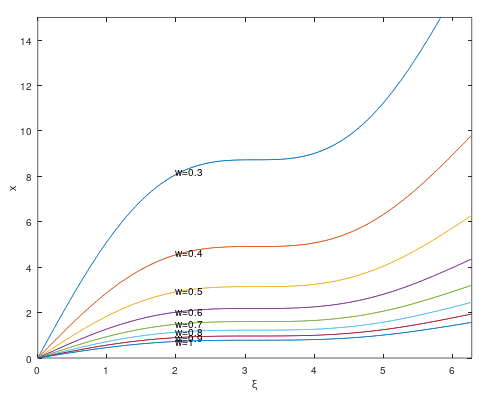
\includegraphics[width=10cm]{chapter_05_paragraph_21_exercice_6}
		\caption{Exemples de trajectoire pour diff\'erentes valeurs de fr\'equence telle que cette derni\`ere ne d\'epende pas de l'amplitude)}\label{FIG:5_21_EX6}
	\end{center}
\end{figure}

\section{Oscillations for\'ees}

Dans les excercices suivants, le syt\`eme se trouve \`a l'\'equilibre et au repos \`a l'instant $t = 0$, i.e. $x(t = 0) = 0$ et $\dot{x}(t = 0) = 0$.

\subsection{Mouvement dans le cas d'une force ext\'erieure non born\'ee dans le temps}

Il s'agit de d\'eterminer les oscillations forc\'ees, $x(t)$, d'un syst\`eme dues \`a une force $F(t)$ dans diff\'erents cas pr\'ecis.

\subsubsection{$F = F_{0}$}\label{PAR:23_EX2a}

Dans ce cas, l'\'equation (\ref{EQ:22_2}) s'\'ecrit :
\benn
	\ddot{x} + \omega^{2}x = \dfrac{F_{0}}{m}
\eenn
dont la solution g\'en\'erale sans second membre peut s'\'ecrire : $a\cos(\omega t + \alpha)$ et une int\'egrale particulière constante, dont la d\'eriv\'ee seconde par rapport au temps est \'evidemment nulle, telle que $\omega^{2}x = \frac{F_{0}}{m} \Leftrightarrow x = \frac{F_{0}}{m\omega^{2}}$. Les conditions initiales permettent de d\'eduire :
\benn
	\begin{cases}
		\dot(x)(0) = 0 \Leftrightarrow -\frac{F_{0}}{m\omega^{2}}\omega\sin\alpha = 0 \Leftrightarrow \sin\alpha = 0 \Leftrightarrow \alpha = 0 \\
		x(0) = 0 \Leftrightarrow a + \frac{F_{0}}{m\omega^{2}} = 0
	\end{cases}
\eenn
ce qui donne comme solution :
\benn
	x(t) = \dfrac{F_{0}}{m\omega^{2}}(1 - \cos(\omega t))
\eenn

\subsubsection{$F = at$}\label{PAR:23_EX2b}

La solution de l'\'equation (\ref{EQ:22_2}) est consiste en :
\begin{itemize}
	\item la solution g\'en\'erale sans second membre : $x_{0} = a\cos(\omega t + \alpha)$
	\item l'int\'egrale particuli\`ere : $x_{1} = bt$ qui permet d'arriver \`a : $0 + \omega^{2}bt = \frac{F_{0}}{m}t \Leftrightarrow b = \frac{F_{0}}{m\omega^{2}}$
\end{itemize}
Les condtions initialies permettent les d\'eductions suivantes :
\benn
	\begin{cases}
		x(0) = 0 \Leftrightarrow \Leftrightarrow a\cos\alpha = 0 \Leftrightarrow \alpha = \pm\frac{\pi}{2} \\
		\dot{x}(0) = 0 \Leftrightarrow -a\omega\sin\alpha + \frac{F_{0}}{m\omega^{2}} = 0 \Leftrightarrow a = \pm\frac{F_{0}}{m\omega^{3}}
	\end{cases}
\eenn
donc :
\benn
	x(t) = \dfrac{F_{0}}{m\omega^{3}}(\omega t + \cos(\omega t \pm \pi/2)) \Leftrightarrow x(t) = \dfrac{F_{0}}{m\omega^{3}}(\omega t \pm \sin(\omega t))
\eenn

\subsubsection{$F = F_{0}e^{-\alpha t}$}

Dans ce cas, l'int\'egrale particuli`ere est de la forme $be^{-\alpha t}$. En l'injectant dans l'\'equation (\ref{EQ:22_2}) :
\benn
	\alpha^{2}be^{-\alpha t} + \omega^{2}be^{-\alpha t} = \dfrac{F_{0}}{m}e^{-\alpha t} \Leftrightarrow b = \dfrac{F_{0}}{m(\omega^{2} + \alpha^{2})}
\eenn
ce qui permet d'\'ecrire le mouvement ainsi :
\benn
	x(t) = a_{1}\cos(\omega t) + a_{2}\sin(\omega t) + \dfrac{F_{0}}{m(\omega^{2} + \alpha^{2})}e^{-\alpha t}
\eenn
Les conditions initiales :
\benn
	\begin{cases}
	x(t = 0) = 0 \Leftrightarrow a_{1} + \dfrac{F_{0}}{m(\omega^{2} + \alpha^{2})} = 0 \Leftrightarrow a_{1} = -\dfrac{F_{0}}{m(\omega^{2} + \alpha^{2})} \\
	\dot{x}(t = 0) = 0 \Leftrightarrow a_{2}\omega - \dfrac{F_{0}\alpha}{m(\omega^{2} + \alpha^{2})} = 0 \Leftrightarrow a_{2} = \dfrac{F_{0}\omega}{m\omega(\omega^{2} + \alpha^{2})}
	\end{cases}
\eenn
permettent de conclure :
\benn
	x(t) = \dfrac{F_{0}}{m(\omega^{2} + \alpha^{2})}\left(e^{-\alpha t} - \cos(\omega t) + \dfrac{\alpha}{\omega}\sin(\omega t)\right)
\eenn

\begin{figure}[htb!]
	\begin{center}
		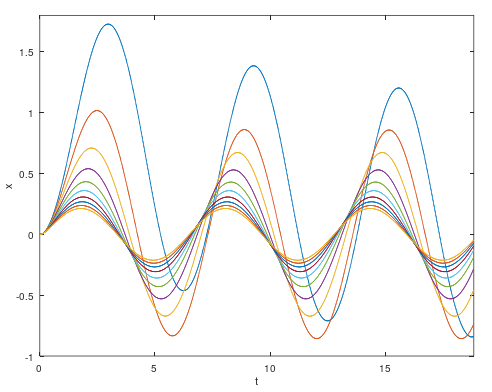
\includegraphics[width=10cm]{chapter_05_paragraph_22_exercice_1c}
		\caption{Oscillations pour $F = F_{0}e^{-\alpha t}$ et $\alpha$ de 0.1 à 5 par pas de 0.5.}\label{FIG:22_1_c}
	\end{center}
\end{figure}

\subsubsection{$F = F_{0}e^{-\alpha t}\cos\beta t$}

Dans ce cas pr\'ecis, en remarquant que $F = \Re{(\overline{F})} = \Re{(F_{0}e^{-\alpha t}e^{i\beta t})} = \Re{(F_{0}e^{(i\beta - \alpha)t})}$, nous utiliserons les formes complexes, alors :
\begin{itemize}
	\item la solution g\'n\'erale sans second membre est $\overline{x_{0}} = \overline{a}e^{i\omega t + \varphi}$
	\item l'int\'egrale particuli\`ere est $\overline{x_{1}} = \overline{b}e^{(i\beta - \alpha)t}$
\end{itemize}
avec $\{a;b\} \in \mathbb{C}$. La relation (\ref{EQ:22_2}) permet d'\'ecrire :
\bea
	\dfrac{F_{0}}{m}e^{i(\beta - \alpha)t} & = & \overline{b}(i\beta - \alpha)^{2}e^{i(\beta - \alpha)t} + \omega^{2}\overline{b}e^{i(\beta - \alpha)t} \Leftrightarrow \overline{b} = \dfrac{F_{0}}{m(\omega^{2} + (i\beta - \alpha)^{2})} \nonumber \\
	\overline{b} & = & \dfrac{F_{0}}{m(\omega^{2} - \beta^{2} + \alpha^{2} - 2i\alpha\beta)} = \dfrac{F_{0}(\omega^{2} - \beta^{2} + \alpha^{2} + 2i\alpha\beta)}{m\left((\omega^{2} - \beta^{2} + \alpha^{2})^{2} + 4\alpha^{2}\beta^{2}\right)} \nonumber
\eea
La solution pour les oscillations forcées dans le domaine complexe s'\'ecrit alors en posant $a = a_{1} + ia_{2}$ avec $\{a_{2};a_{2}\} \in \mathbb{R}$ :
\bea
	\overline{x} & = & \dfrac{F_{0}(\omega^{2} - \beta^{2} + \alpha^{2} + 2i\alpha\beta)}{m\left((\omega^{2} - \beta^{2} + \alpha^{2})^{2} + 4\alpha^{2}\beta^{2}\right)}e^{(i\beta - \alpha)t}(\cos(\beta t) + i\sin(\beta t)) \nonumber \\
	& & + (a_{1} + ia_{2})\cos(\omega t) + (-a_{2} + ia_{1})\sin(\omega t) \nonumber
\eea
En effet, dans la solution g\'en\'erale sans second membre, l'expression exponentielle se d\'eveloppe ainsi :
\bea
	e^{i\omega t + \varphi} & = & \cos(\omega t + \varphi) + i\sin(\omega t + \varphi) = \cos(\omega t)\cos\varphi - \sin(\omega t)\sin\varphi \nonumber \\
	& &	+ i(\cos(\omega t)\sin\varphi + \sin(\omega t)\cos\varphi) \nonumber \\
	& = & (\cos\varphi + i\sin\varphi)\cos(\omega t) + (-\sin\varphi + i\cos\varphi)\sin(\omega t) \nonumber
\eea
et les facteurs $a_{1}$ et $a_{2}$ permettent de d\'efinir la phase. Ainsi :
\bea
	\overline{x} & = & a_{1}\cos(\omega t) - a_{2}\sin(\omega t) + \dfrac{F_{0}(\omega^{2} - \beta^{2} + \alpha^{2})}{m\left((\omega^{2} - \beta^{2} + \alpha^{2})^{2} \nonumber + 4\alpha^{2}\beta^{2}\right)}e^{-\alpha t}\cos(\beta t) \nonumber \\
	& & - \dfrac{2F_{0}\alpha\beta}{m\left((\omega^{2} - \beta^{2} + \alpha^{2})^{2} + 4\alpha^{2}\beta^{2}\right)}e^{-\alpha t}\sin(\beta t) \nonumber \\
	& & + i\left(a_{2}\cos(\omega t) + a_{1}\sin(\omega t) + \dfrac{F_{0}(\omega^{2} - \beta^{2} + \alpha^{2})}{m\left((\omega^{2} - \beta^{2} + \alpha^{2})^{2} + 4\alpha^{2}\beta^{2}\right)}e^{-\alpha t}\sin(\beta t) \right. \nonumber \\
	& & + \left. \dfrac{2F_{0}\alpha\beta}{m\left((\omega^{2} - \beta^{2} + \alpha^{2})^{2} + 4\alpha^{2}\beta^{2}\right)}e^{-\alpha t}\cos(\beta t)\right) \nonumber
\eea
Cette expression se r\'eduit car le mouvement oscillatoire est r\'ealis\'e dans le domaine r\'eel, aussi $x = \Re{(\overline{x})}$. Les conditions initiales permettent de d\'eduire les c{\oe}fficients tels que :
\benn
	x(t = 0) = 0 \Leftrightarrow a_{1} + \dfrac{F_{0}(\omega^{2} - \beta^{2} + \alpha^{2})}{m\left((\omega^{2} - \beta^{2} + \alpha^{2})^{2} + 4\alpha^{2}\beta^{2}\right)} = 0
\eenn
et :
\bea
	\dot{x} & = & -a_{1}\omega\sin(\omega t) - a_{2}\omega\cos(\omega t) + \dfrac{F_{0}(\omega^{2} - \beta^{2} + \alpha^{2})}{m\left((\omega^{2} - \beta^{2} + \alpha^{2})^{2} + 4\alpha^{2}\beta^{2}\right)}\left(-\alpha e^{-\alpha t}\cos(\beta t) - \beta e^{-\alpha t}\sin(\beta t)\right)\nonumber \\
	& & - \dfrac{2F_{0}\alpha\beta}{m\left((\omega^{2} - \beta^{2} + \alpha^{2})^{2} + 4\alpha^{2}\beta^{2}\right)}\left(-\alpha e^{-\alpha t}\sin(\beta t) + \beta e^{-\alpha t}\cos(\beta t)\right) \nonumber
\eea
Donc :
\bea
	0 & = & -a_{2}\omega - \dfrac{\alpha F_{0}(\omega^{2} - \beta^{2} + \alpha^{2})}{m\left((\omega^{2} - \beta^{2} + \alpha^{2})^{2} + 4\alpha^{2}\beta^{2}\right)} - \dfrac{2F_{0}\alpha\beta^{2}}{m\left((\omega^{2} - \beta^{2} + \alpha^{2})^{2} + 4\alpha^{2}\beta^{2}\right)} \nonumber \\
	\Leftrightarrow a_{2} & = & -\dfrac{\alpha F_{0}(\omega^{2} + \alpha^{2} + \beta^{2})}{m\omega\left((\omega^{2} - \beta^{2} + \alpha^{2})^{2} + 4\alpha^{2}\beta^{2}\right)} \nonumber
\eea
Ainsi le mouvement est d\'ecrit par :
\bea
	x(t) & = & \dfrac{F_{0}(\omega^{2} + \alpha^{2} + \beta^{2})}{m\left((\omega^{2} - \beta^{2} + \alpha^{2})^{2} + 4\alpha^{2}\beta^{2}\right)} \left(-(\omega^{2} - \beta^{2} + \alpha^{2})\cos(\omega t) + \dfrac{\alpha}{\omega}(\omega^{2} + \alpha^{2} + \beta^{2})\sin(\omega t) \right. \nonumber \\
	& & + \left. (\omega^{2} - \beta^{2} + \alpha^{2})\cos(\beta t) -2\alpha\beta\sin(\beta t)e^{-\alpha t}\right) \nonumber
\eea

\begin{figure}[htb!]
	\begin{center}
		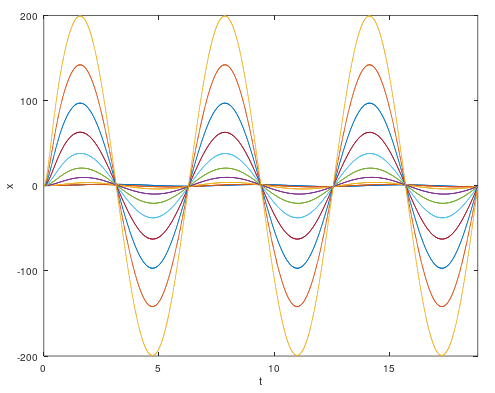
\includegraphics[width=10cm]{chapter_05_paragraph_22_exercice_1d}
		\caption{Oscillations pour $F = F_{0}e^{-\alpha t}\cos\beta t$ en supposant $\alpha = \beta$ et $\alpha$ de 1 à 5 par pas de 0.5.}\label{FIG:22_1_d}
	\end{center}
\end{figure}

\subsection{Mouvement dans le cas d'une force ext\'erieure born\'ee dans le temps}

Dans cette suite d'exercices, l'objectif est de calculer l'amplitude finale des oscillations d'un système apr\`es l'action d'une force ext\'erieure telle que $F = 0$ pour $t < 0$ et qu'\`a $t = 0$, le syt\`eme est au repos et \`a l'\'equilibre, i.e. $x(t = 0) = 0$ et $\dot{x}(t = 0) = 0$.

\subsubsection{Premier exemple}

Dans ce premier cas, la force ext\'erieure s'exprime telle que :
\begin{itemize}
	\item $F = F_{0}t/T$ pour $t \in [0;T]$
	\item $F = F_{0}$ pour $t > T$
\end{itemize}

Pour $0 < t < T$, nous pouvons repartir de la solution du probl\`eme (\ref{PAR:23_EX2b}) avec ici $a = F_{0}/T$. Aussi, nous avons dans cet intervalle de temps :
\benn
	x(t) = \dfrac{F_{0}}{m\omega^{3}T}(\omega t - \sin(\omega t))
\eenn
Pour $t \ge T$, c'est la solution du probl\`eme (\ref{PAR:23_EX2a}) qui peut \^etre utilis\'ee, \`a savoir $x(t) = a\cos(\omega t + \alpha) + \frac{F_{0}}{m\omega^{2}}$. Il reste \`a remplir les conditions de continuit\'e pour $t = T$, soit :
\benn
	\begin{cases}
		\dfrac{F_{0}}{m\omega^{3}T}(\omega T - \sin(\omega T)) = a\cos(\omega T + \alpha) + \dfrac{F_{0}}{m\omega^{2}} \Leftrightarrow a\cos(\omega T + \alpha) = -\dfrac{F_{0}}{m\omega^{3}T}\sin(\omega T) \\
		\\
		\dfrac{F_{0}}{m\omega^{3}T}(\omega - \omega\cos(\omega T)) = -a\omega\sin(\omega T + \alpha) \Leftrightarrow a\sin(\omega T + \alpha) = \dfrac{F_{0}}{m\omega^{3}T}(1 - \cos(\omega T))
	\end{cases}
\eenn
En appliquant l'identit\'e $\cos^{2} + \sin^{2} = 1$, cela permet d'en d\'eduire l'amplitude des oscillations :
\bea
	a^{2} & = & \left(-\dfrac{F_{0}}{m\omega^{3}T}\sin(\omega T)\right)^{2} + \left(\dfrac{F_{0}}{m\omega^{3}T}(1 - \cos(\omega T))\right)^{2} \nonumber \\
	& = & \left(\dfrac{F_{0}}{m\omega^{3}T}\right)^{2}\left(\sin^{2}(\omega T) + 1 + \cos^{2}(\omega T) - 2\cos(\omega T)\right) \nonumber \\
	& = & 2\left(\dfrac{F_{0}}{m\omega^{3}T}\right)^{2}(1 - \cos(\omega T)) = 4\left(\dfrac{F_{0}}{m\omega^{3}}\right)^{2}\sin^{2}\left(\dfrac{\omega T}{2}\right) \nonumber \\
	\Leftrightarrow a & = & 2\left(\dfrac{F_{0}}{m\omega^{3}T}\right)\bigg\lvert\sin\left(\dfrac{\omega T}{2}\right)\bigg\rvert \nonumber
\eea

\begin{figure}[htb!]
	\begin{center}
		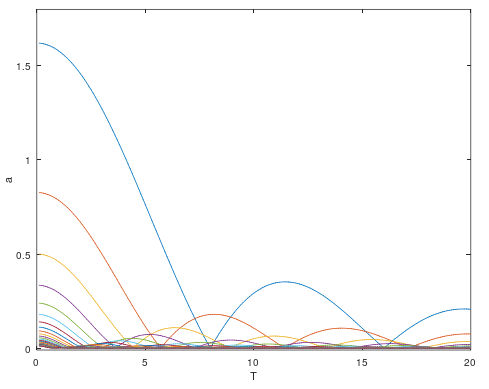
\includegraphics[width=10cm]{chapter_05_paragraph_22_exercice_2}
		\caption{\'Evolution de l'amplitude en fonction de la période pour $\omega$ de $\pi/4$ à $3\pi$}\label{FIG:22_2}
	\end{center}
\end{figure}

\subsubsection{Deuxi\`eme exemple}

Dans ce deuxi\`eme cas, la force ext\'erieure s'exprime telle que :
\begin{itemize}
	\item $F = F_{0}$ pour $t \in [0;T]$
	\item $F = 0$ pour $t > T$
\end{itemize}

La force ext\'erieure n'op\`ere plus pour $t > T$ aussi l'amplitude des oscillations au-del\`a de $T$ est exactement la valeur de l'oscillation \`a $t = T$. En reprenant la solution du probl\`eme (\ref{PAR:23_EX2a}) pour $t < T$ et appliqu\'ee en $t = T$, nous obtenons ais\'ement :
\benn
	a = x(T) = \dfrac{F_{0}}{m\omega^{2}}(1 - \cos(\omega T)) = 2\dfrac{F_{0}}{m\omega^{2}}\sin^{2}\left(\dfrac{\omega T}{2}\right)
\eenn
Ce r\'esultat est diff\'erent de celui pr\'esent\'e dans le livre en $\propto \sin$ au lieu de $\propto \sin^{2}$ ici obtenu.

\subsubsection{Troisi\`eme exemple}

Dans ce troisi\`eme cas, la force ext\'erieure s'exprime telle que :
\begin{itemize}
	\item $F = F_{0}t/T$ pour $t \in [0;T]$
	\item $F = 0$ pour $t > T$
\end{itemize}

Pour cet exemple, nous allons raisonner avec la variable d\'efinie en (\ref{EQ:22_9}), \`a savoir $\xi = \dot{x} + i\omega x$. Sans force ext\'erieure, i.e. pour la partie telle que $t > T$, la relation (\ref{EQ:22_10}) permet de d\'eduire l'\'energie du syst\`eme comme $\frac{1}{2}m\omega^{2}a^{2}$ alors qu'avec l'application d'une force ext\'erieure, nous avons vu par l'\'equation (\ref{EQ:22_11}) que l'\'energie du syst\`eme s'\'ecrit $\frac{1}{2}m\lvert\xi\rvert^{2}$ et en particulier $\frac{1}{2}m\lvert\xi(T)\rvert^{2}$. Comme l'\'energie du syst\`eme se conserve, nous pouvons en conclure que :
\benn
	\lvert\xi(T)\rvert^{2} = \omega^{2}a^{2}
\eenn
Pour $0 < t < T$, la solution du probl\`eme est celle du paragraphe (\ref{PAR:23_EX2b}) qui permet d'\'ecrire $x(t) = \frac{F_{0}}{m\omega^{3}T}(\omega t - \sin(\omega t))$. Nous avons alors :
\bea
	\xi & = & \dot{x} + i\omega x = \dfrac{F_{0}}{m\omega^{3}T}(\omega - \omega\cos(\omega t)) + i\omega\dfrac{F_{0}}{m\omega^{3}T}(\omega t - \sin(\omega t)) \nonumber \\
	& = & \dfrac{F_{0}}{m\omega^{2}T}(1 - \cos(\omega t)) + i\dfrac{F_{0}}{m\omega^{2}T}(\omega t - \sin(\omega t)) = \dfrac{F_{0}}{m\omega^{2}T}(1 - \cos(\omega t) + i(\omega t - \sin(\omega t)) \nonumber \\
	\Leftrightarrow \lvert\xi(T)\rvert^{2} & = & \dfrac{F_{0}^{2}}{m^{2}\omega^{4}T^{2}}\left((1 - \cos(\omega T)^{2} + (\omega T - \sin(\omega T))^{2}\right) \nonumber \\
	& = & \dfrac{F_{0}^{2}}{m^{2}\omega^{4}T^{2}}\left(1 + \cos^{2}(\omega T) - 2\cos(\omega T) + \omega^{2}T^{2} + \sin^{2}(\omega t) - 2\omega T\sin(\omega T)\right) \nonumber \\
	& = & \dfrac{F_{0}^{2}}{m^{2}\omega^{4}T^{2}}\left(\omega^{2}T^{2} - 2\omega T\sin(\omega T) + 2(1 - \cos(\omega T))\right) \nonumber
\eea
En reprenant l'\'egalit\'e $\lvert\xi(T)\rvert^{2} = \omega^{2}a^{2}$, nous arrivons alors :
\benn
	a = \dfrac{F_{0}}{m\omega^{3}T}\sqrt{\omega^{2}T^{2} - 2\omega T\sin(\omega T) + 2(1 - \cos(\omega T))}
\eenn

\begin{figure}[htb!]
	\begin{center}
		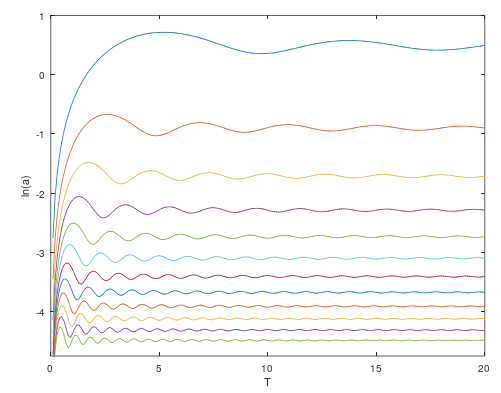
\includegraphics[width=10cm]{chapter_05_paragraph_22_exercice_4}
		\caption{\'Evolution de l'amplitude en fonction de la période pour $\omega$ de $\pi/4$ à $3\pi$}\label{FIG:22_4}
	\end{center}
\end{figure}

\subsubsection{Quatri\`eme exemple}

Dans ce dernier cas, la force ext\'erieure s'exprime telle que :
\begin{itemize}
	\item $F = F_{0}\sin(\omega t)$ pour $t \in [0;T]$
	\item $F = 0$ pour $t > T = 2\pi/\omega$
\end{itemize}
ainsi l'exercice de la force ext\'erieure ainsi que la dur\'ee d\'ependent d'ors et d\'ej\`a de la fr\'equence propre du syst\`eme. Par d\'efinition, $\sin(\omega t) = (e^{i\omega t} - e^{-i\omega t})/2i$ donc nous pouvons \'ecrire la force ext\'erieure comme $F(t) = \frac{F_{0}}{2i}(e^{i\omega t} - e^{-i\omega t})$ pour $t < T$. Les conditions initiales retenues impliquent que $\xi(t = 0) = 0$ aussi la relation (\ref{EQ:22_10}) donne :
\bea
	\xi(T) & = & \dfrac{F_{0}}{2mi}e^{i\omega T}\int_{0}^{T}\left(e^{i\omega t} - e^{-i\omega t}\right)e^{-i\omega t}\mathrm{d}t = \dfrac{F_{0}}{2mi}e^{i\omega T}\int_{0}^{T}\left(1 - e^{-2i\omega t}\right)\mathrm{d}t \nonumber \\
	& = & \dfrac{F_{0}}{2mi}e^{i\omega T}\left(T + \dfrac{1}{2i\omega}\left(e^{-2i\omega T} - 1\right)\right) = -\dfrac{F_{0}}{2m}ie^{i\omega T}\left(T - \dfrac{i}{2\omega}\left(e^{-2i\omega T} - 1\right)\right) \nonumber
\eea
or $T = 2\pi/\omega$ et $\forall n \in \mathbb{Z}\text{, }e^{2in\pi} = 1$ donc :
\bea
	\xi(T) & = & -\dfrac{F_{0}}{2m}ie^{2\pi i}\left(\dfrac{2\pi}{\omega} - \dfrac{i}{2\omega}\left(e^{-4\pi i} - 1\right)\right) = -\dfrac{F_{0}\pi}{m\omega}i \nonumber \\
	\Leftrightarrow \lvert\xi(T)\rvert^{2} & = & \dfrac{F_{0}^{2}\pi^{2}}{m^{2}\omega^{2}} = a^{2}\omega^{2} \Leftrightarrow a = \dfrac{\pi F_{0}}{m\omega^{2}} \nonumber
\eea

\section{Syst\`emes \`a plusieurs degr\'es de libert\'e}

\subsection{Cas d'une fonction de Lagrange donn\'ee et pour deux degr\'es de libert\'e}

L'objectif de ce probl\`eme est de d\'eterminer les oscillations du syst\`eme dont la fonction de Lagrange est :
\benn
	L = \dfrac{1}{2}(\dot{x}^{2} + \dot{y}^{2}) - \dfrac{\omega_{0}^{2}}{2}(x^{2} + y^{2}) +\alpha xy
\eenn
correspondant à deux syst\`emes lin\'eaires identiques de fr\'equence propre $\omega_{0}$ coupl\'es par une interaction d\'efinie par $-\alpha xy$. Les \'equations du mouvement d\'efinies par les relations (\ref{EQ:2_6}) sont :
\benn
	\begin{cases}
		\dfrac{\mathrm{d}}{\mathrm{dt}}\left(\dfrac{\partial L}{\partial\dot{x}}\right) = \dfrac{\partial L}{\partial x} \Leftrightarrow \dfrac{\mathrm{d}\dot{x}}{\mathrm{dt}} = -\omega_{0}^{2}x + \alpha y \Leftrightarrow \ddot{x} + \omega_{0}^{2}x = \alpha y \\
		\\
		\dfrac{\mathrm{d}}{\mathrm{dt}}\left(\dfrac{\partial L}{\partial\dot{y}}\right) = \dfrac{\partial L}{\partial y} \Leftrightarrow \dfrac{\mathrm{d}\dot{y}}{\mathrm{dt}} = -\omega_{0}^{2}y + \alpha x \Leftrightarrow \ddot{y} + \omega_{0}^{2}y = \alpha x
	\end{cases}
\eenn
En posant $x = A_{x}e^{i\omega t}$ et $y = A_{y}e^{i\omega t}$, le syst\`eme d'\'equations devient :
\benn
	\begin{cases}
		-\omega^{2}A_{x} + \omega_{0}^{2}A_{x} = \alpha A_{y} \Leftrightarrow A_{x}(\omega_{0}^{2} - \omega^{2}) = \alpha A_{y} \\
		-\omega^{2}A_{y} + \omega_{0}^{2}A_{y} = \alpha A_{x} \Leftrightarrow A_{y}(\omega_{0}^{2} - \omega^{2}) = \alpha A_{x}
	\end{cases}
\eenn
L'\'equation caract\'eristique est le d\'eterminant \'egal \`a 0 de la matrice correspondant au syst\`eme d'\'equations ci-dessus, soit :
\benn
	(\omega_{0}^{2} - \omega^{2})^{2} - \alpha^{2} = 0 \Leftrightarrow \omega_{1}^{2} = \omega_{0}^{2} + \alpha\text{ et }\omega_{2}^{2} = \omega_{0}^{2} - \alpha
\eenn
En prenant, $\omega^{2} = \omega_{1}^{2}$ nous obtenons $A_{x} = A_{y}$ alors que pour $\omega^{2} = \omega_{2}^{2}$, nous avons $A_{x} = -A_{y}$. Cela permet d'introduire les coordonn\'ees normales $Q_{1}$ et $Q_{2}$ telles que :
\benn
	\begin{cases}
		x = \dfrac{1}{\sqrt{2}}(Q_{1} + Q_{2}) \\
		x = \dfrac{1}{\sqrt{2}}(Q_{1} - Q_{2})
	\end{cases}
\eenn
Les c{\oe}fficients $1/\sqrt{2}$ permettent d'obtenir les c{\oe}fficient $1/2$ devant les carr\'es des vitesses dans la fonction de Lagrange du syst\`eme.

Dans le cas particulier o\`u $\alpha \ll \omega^{2}$ alors $\omega^{2} = \omega_{0}^{2} \pm \alpha = \omega_{0}^{2}(1 \pm \alpha/\omega_{0}^{2}) \approx \omega_{0}^{2}(1 \pm \alpha/(2\omega_{0}))$. Les degr\'es de libert\'e $x$ et $y$ sont l'addition de deux oscillations de fr\'equence voisine, avec un battement de $\omega_{2} - \omega_{1} = \alpha/\omega_{0}$.

\subsection{Oscillations d'un pendule double oscillant dans un plan}

Dans cet exercice, nous reprenons le pendule double introduit dans le paragraphe (\ref{PAR:5_EX1}) et illustr\'e sur la figure (\ref{FIG:1_1})) pour lequel la fonction de Lagrange du syst\`eme est :
\benn
	L = \dfrac{m_{1}+m_{2}}{2}l_{1}^{2}\dot{\varphi_{1}}^{2} + \dfrac{m_{2}}{2}l_{2}^{2}\dot{\varphi_{2}}^{2} + m_{2}l_{1}l_{2}\cos(\varphi_{1} - \varphi_{2})\dot{\varphi_{1}}\dot{\varphi_{2}} + (m_{1}+m_{2})gl_{1}\cos(\varphi_{1}) + m_{2}gl_{2}\cos(\varphi_{2})
\eenn
Dans le cadre des petites oscillations qui nous occupe, i.e. $\varphi_{1} \ll 1$ et $\varphi_{2} \ll 1$, la fonction de Lagrange se r\'eduit \`a :
\benn
	L = \dfrac{m_{1}+m_{2}}{2}l_{1}^{2}\dot{\varphi_{1}}^{2} + \dfrac{m_{2}}{2}l_{2}^{2}\dot{\varphi_{2}}^{2} - \dfrac{(m_{1} + m_{2})}{2}gl_{1}\varphi_{1}^{2} - m_{2}gl_{2}\varphi_{2}^{2}
\eenn
car $\cos\varphi \approx \cos(0) - (\varphi - 0)\sin(0) - \frac{1}{2}(\varphi - 0)^{2}\cos(0) \approx \frac{1}{2}\varphi^{2}$. En application des \'equations du mouvement (\ref{EQ:2_6}), nous obtenons :
\bea
	\dfrac{\mathrm{d}}{\mathrm{dt}}\left(\dfrac{\partial L}{\partial\dot{\varphi_{1}}}\right) = \dfrac{\partial L}{\partial \varphi_{1}} \Leftrightarrow \dfrac{\mathrm{d}}{\mathrm{dt}}\left((m_{1} + m_{2})l_{1}^{2}\dot{\varphi}_{1} + m_{2}l_{1}l_{2}\dot{\varphi}_{2}\right) & = & -(m_{1} + m_{2})gl_{1}\varphi_{1} \nonumber \\
	\Leftrightarrow (m_{1} + m_{2})l_{1}^{2}\ddot{\varphi}_{1} + m_{2}l_{1}l_{2}\ddot{\varphi}_{2} + (m_{1} + m_{2})gl_{1}\varphi_{1} & = & 0 \nonumber \\
	\Leftrightarrow (m_{1} + m_{2})l_{1}\ddot{\varphi}_{1} + m_{2}l_{2}\ddot{\varphi}_{2} + (m_{1} + m_{2})g\varphi_{1} & = & 0 \nonumber
\eea
et :
\bea
	\dfrac{\mathrm{d}}{\mathrm{dt}}\left(\dfrac{\partial L}{\partial\dot{\varphi_{2}}}\right) = \dfrac{\partial L}{\partial \varphi_{2}} \Leftrightarrow \dfrac{\mathrm{d}}{\mathrm{dt}}\left(m_{2}l_{2}^{2}\dot{\varphi}_{2} + m_{2}l_{1}l_{2}\dot{\varphi}_{1}\right) & = &  -m_{2}gl_{2}\varphi_{2} \nonumber \\
	\Leftrightarrow m_{2}l_{2}^{2}\ddot{\varphi}_{2} + m_{2}l_{1}l_{2}\ddot{\varphi}_{1} + m_{2}gl_{2}\varphi_{2} & = & 0 \nonumber \\
	\Leftrightarrow m_{2}l_{2}\ddot{\varphi}_{2} + m_{2}l_{1}\ddot{\varphi}_{1} + m_{2}g\varphi_{2} & = & 0 \nonumber
\eea
En posant $\varphi_{1} = A_{1}e^{i\omega t}$ et $\varphi_{2} = A_{2}e^{i\omega t}$, nous obtenons :
\benn
	\begin{cases}
		-(m_{1} + m_{2})l_{1}A_{1}\omega^{2} - m_{2}l_{2}\omega^{2}A_{2} + (m_{1} + m_{2})gA_{1} = 0 \\
		-l_{2}\omega^{2}A_{2} - l_{1}\omega^{2}A_{1} + gA_{2} = 0
	\end{cases}
\eenn
\benn
	\Leftrightarrow
	\begin{cases}
		(g - l_{1}\omega^{2})(m_{1} + m_{2})A_{1} - m_{2}l_{2}\omega^{2}A_{2} = 0 \\
		-l_{1}\omega^{2}A_{1} + (g - l_{2}\omega^{2})A_{2} = 0
	\end{cases}
\eenn
L'\'equation caract\'eristique du syst\`eme est alors :
\bea
	(g - l_{1}\omega^{2})(g - l_{2}\omega^{2})(m_{1} + m_{2}) - m_{2}l_{1}l_{2}\omega^{4} & = & 0 \nonumber \\
	(m_{1} + m_{2})(g^{2} - (l_{1} + l_{2})g\omega^{2} + l_{1}l_{2}\omega^{4}) - m_{2}l_{1}l_{2}\omega^{4} & = & 0 \nonumber \\
	m_{1}l_{1}l_{2}\omega^{4} - (m_{1} + m_{2})(l_{1} + l_{2})g\omega^{2} + (m_{1} + m_{2})g^{2} & = & 0 \nonumber
\eea
et ses deux solutions sont :
\bea
	\omega^{2} & = & \dfrac{(m_{1} + m_{2})(l_{1} + l_{2})g \pm \sqrt{(m_{1} + m_{2})^{2}(l_{1} + l_{2})^{2}g^{2} - 4m_{1}(m_{1} + m_{2})l_{1}l_{2}g^{2}}}{2m_{1}l_{1}l_{2}} \nonumber \\
	& = & \dfrac{g}{2m_{1}l_{1}l_{2}}\left[(m_{1} + m_{2})(l_{1} + l_{2}) \pm \sqrt{(m_{1} + m_{2})\left[(m_{1} + m_{2})(l_{1} + l_{2})^{2} - 4m_{1}l_{1}l_{2}\right]} \right] \nonumber
\eea

\begin{figure}[htb!]
	\begin{center}
		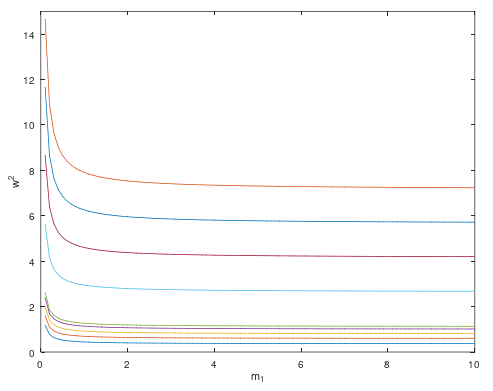
\includegraphics[width=10cm]{chapter_05_paragraph_23_exercice_2}
		\caption{Exemple de variation de la solution $\omega^{2}$ << + >> en supposant $l_{2} = 2l_{1}$ et pour un rapport $m_{2}/m_{1}$ allant de $0.1$ à $10$.}\label{FIG:23_2}
	\end{center}
\end{figure}

\subsection{Trajectoire dans un champ central $\propto r^{2}$}\label{PAR:23_EX3}

La trajectoire d'une particule dans un champ telle que l'\'energie potentielle $U$ soit \'egale \`a $\frac{kr^{2}}{2} = \frac{k(x^{2} + y^{2}}{2}$ s'effectue dans un plan. La relation (\ref{EQ:23_15}) donne pour la fonction de Lagrange de la particule :
\benn
	L = \dfrac{m}{2}(\dot{x}^{2} + \dot{y}^{2}) - \dfrac{k}{2}(x^{2} + y^{2})
\eenn
ce qui donne pour les \'equations du mouvement, voir (\ref{EQ:2_6}) :
\benn
	\begin{cases}
		\dfrac{\mathrm{d}}{\mathrm{dt}}\left(\dfrac{\partial L}{\partial\dot{x}}\right) = \dfrac{\partial L}{\partial x} \Leftrightarrow m\ddot{x} + kx = 0 \\
		\dfrac{\mathrm{d}}{\mathrm{dt}}\left(\dfrac{\partial L}{\partial\dot{y}}\right) = \dfrac{\partial L}{\partial y} \Leftrightarrow m\ddot{y} + ky = 0
	\end{cases}
\eenn
En posant $x = A_{x}e^{i\omega t}$ et $y = A_{y}e^{i\omega t}$, le syst\`eme d'\'equations devient :
\benn
	\begin{cases}
		-m\omega^{2}A_{x} + kA_{x} = 0 \\
		-m\omega^{2}A_{y} + kA_{y} = 0
	\end{cases}
\eenn
ce qui nous donne directement $\omega^{2} = \sqrt{k/m}$. En posant $x = a\cos(\omega t)$ et $y = b\cos(\omega t + \alpha) = b\cos(\omega t)\cos\alpha - b\sin(\omega t)\sin\alpha$, sachant que $y$ peut \^etre d\'ephas\'e par rapport \`a $x$, alors :
\benn
	\cos(\omega t) = \dfrac{x}{a}\text{ et }\sin(\omega t) = \dfrac{b\cos(\omega t)\cos\alpha - y}{b\sin\alpha} = \dfrac{bx\cos\alpha - ay}{ab\sin\alpha}
\eenn
Enfin, en s'appuyant sur l'\'egalit\'e $\cos^{2}(\omega t) + \sin^{2}(\omega t) = 1$, nous pouvons \'ecrire :
\bea
	\dfrac{x^{2}}{a^{2}} + \dfrac{b^{2}x^{2}\cos^{2}\alpha + a^{2}y^{2} - 2abxy\cos\alpha}{a^{2}b^{2}\sin^{2}\alpha} & = & 1 \nonumber \\
	b^{2}x^{2}\sin^{2}\alpha + b^{2}x^{2}\cos^{2}\alpha + a^{2}y^{2} - 2abxy\cos\alpha & = & a^{2}b^{2}\sin^{2}\alpha \nonumber \\
	b^{2}x^{2} + a^{2}y^{2} - 2abxy\cos\alpha = a^{2}b^{2}\sin^{2}\alpha \Leftrightarrow \dfrac{x^{2}}{a^{2}} + \dfrac{y^{2}}{a^{2}} - \dfrac{2xy}{ab}\cos\alpha & = & \sin^{2}\alpha \nonumber
\eea
qui correspond \`a une ellipse dont le centre est positionn\'e \`a l'origine des coordonn\'ees.

\section{Oscillations des mol\'ecules}

Dans les trois probl\`emes suivants, il s'agit de trouver les fr\'equences des oscillations lin\'eaires.

\subsection{Cas d'une mol\'ecule lin\'eaire sym\'etrique}

\begin{figure}[htb!]
	\begin{center}
		\begin{picture}(200,150)(0,0)
			%molecule #1
			\linethickness{0.05mm}
			\put(23,150){\line(1,0){150}}
			\put(22,154){$1$}
			\put(25,150){\circle*{5}}
			\put(20,138){$A$}
			\put(62,152){$l$}
			\put(97,154){$2$}
			\put(100,150){\circle*{5}}
			\put(95,138){$B$}
			\put(137,152){$l$}
			\put(172,154){$3$}
			\put(175,150){\circle*{5}}
			\put(170,138){$C$}
			%molecule #2
			\put(0,97){a)}
			\linethickness{0.05mm}
			\put(25,100){\line(1,0){150}}
			\put(25,150){\circle*{5}}
			\put(100,150){\circle*{5}}
			\put(175,150){\circle*{5}}
			\linethickness{0.5mm}
			\put(25,100){\vector(1,0){15}}
			\put(175,100){\vector(-1,0){15}}
			%molecule #3
			\put(0,47){b)}
			\linethickness{0.05mm}
			\put(25,50){\line(1,0){150}}
			\put(25,150){\circle*{5}}
			\put(100,150){\circle*{5}}
			\put(175,150){\circle*{5}}
			\linethickness{0.5mm}
			\put(25,50){\vector(-1,0){15}}
			\put(175,50){\vector(1,0){15}}
			%molecule #4
			\put(0,-3){c)}
			\linethickness{0.05mm}
			\put(25,0){\line(1,0){150}}
			\put(25,150){\circle*{5}}
			\put(100,150){\circle*{5}}
			\put(175,150){\circle*{5}}
			\linethickness{0.5mm}
			\put(25,0){\vector(0,-1){15}}
			\put(100,0){\vector(0,1){15}}
			\put(175,0){\vector(0,-1){15}}
		\end{picture}
		\caption{Cas d'oscillations lin\'eaires pour une mol\'ecule triatomique sym\'etrique}\label{FIG:28_EX24_1}
	\end{center}
\end{figure}

Dans ce cas de figure, la rotation n'a pas de sens mais par contre, la mol\'ecule peut tr\`es bien avoir un mouvement de translation. Aussi, il est pr\'ef\'erable de calculer dans le cadre du r\'ef\'erentiel du centre d'inertie.

\subsubsection{Oscillations longitudinales}

La relation (\ref{EQ:24_1}) permet d'\'etablir :
\benn
	m_{A}x_{1} + m_{B}x_{2} + m_{C}x_{3} = 0 \Leftrightarrow x_{2} = -\dfrac{m_{A}}{m_{B}}(x_{1} + x_{3})
\eenn
La fonction de Lagrange se compose de :
\benn
	L = \dfrac{1}{2}m_{A}\dot{x}_{1}^{2} + \dfrac{1}{2}m_{B}\dot{x}_{2}^{2} + \dfrac{1}{2}m_{A}\dot{x}_{3}^{2} - \dfrac{k_{l}}{2}(x_{1} - x_{2})^{2} - \dfrac{k_{l}}{2}(x_{3} - x_{2})^{2}
\eenn
avec $k_{l}$ est le c{\oe}fficient longitudinal.

\subsubsection{Oscillations transversales}

\subsection{Cas d'une mol\'ecule triangulaire}

\subsection{Cas d'une mol\'ecule lin\'eaire asym\'etrique}

\end{document}
